\documentclass[twoside]{book}

% Packages required by doxygen
\usepackage{fixltx2e}
\usepackage{calc}
\usepackage{doxygen}
\usepackage[export]{adjustbox} % also loads graphicx
\usepackage{graphicx}
\usepackage[utf8]{inputenc}
\usepackage{makeidx}
\usepackage{multicol}
\usepackage{multirow}
\PassOptionsToPackage{warn}{textcomp}
\usepackage{textcomp}
\usepackage[nointegrals]{wasysym}
\usepackage[table]{xcolor}

% Font selection
\usepackage[T1]{fontenc}
\usepackage[scaled=.90]{helvet}
\usepackage{courier}
\usepackage{amssymb}
\usepackage{sectsty}
\renewcommand{\familydefault}{\sfdefault}
\allsectionsfont{%
  \fontseries{bc}\selectfont%
  \color{darkgray}%
}
\renewcommand{\DoxyLabelFont}{%
  \fontseries{bc}\selectfont%
  \color{darkgray}%
}
\newcommand{\+}{\discretionary{\mbox{\scriptsize$\hookleftarrow$}}{}{}}

% Page & text layout
\usepackage{geometry}
\geometry{%
  a4paper,%
  top=2.5cm,%
  bottom=2.5cm,%
  left=2.5cm,%
  right=2.5cm%
}
\tolerance=750
\hfuzz=15pt
\hbadness=750
\setlength{\emergencystretch}{15pt}
\setlength{\parindent}{0cm}
\setlength{\parskip}{3ex plus 2ex minus 2ex}
\makeatletter
\renewcommand{\paragraph}{%
  \@startsection{paragraph}{4}{0ex}{-1.0ex}{1.0ex}{%
    \normalfont\normalsize\bfseries\SS@parafont%
  }%
}
\renewcommand{\subparagraph}{%
  \@startsection{subparagraph}{5}{0ex}{-1.0ex}{1.0ex}{%
    \normalfont\normalsize\bfseries\SS@subparafont%
  }%
}
\makeatother

% Headers & footers
\usepackage{fancyhdr}
\pagestyle{fancyplain}
\fancyhead[LE]{\fancyplain{}{\bfseries\thepage}}
\fancyhead[CE]{\fancyplain{}{}}
\fancyhead[RE]{\fancyplain{}{\bfseries\leftmark}}
\fancyhead[LO]{\fancyplain{}{\bfseries\rightmark}}
\fancyhead[CO]{\fancyplain{}{}}
\fancyhead[RO]{\fancyplain{}{\bfseries\thepage}}
\fancyfoot[LE]{\fancyplain{}{}}
\fancyfoot[CE]{\fancyplain{}{}}
\fancyfoot[RE]{\fancyplain{}{\bfseries\scriptsize Generated by Doxygen }}
\fancyfoot[LO]{\fancyplain{}{\bfseries\scriptsize Generated by Doxygen }}
\fancyfoot[CO]{\fancyplain{}{}}
\fancyfoot[RO]{\fancyplain{}{}}
\renewcommand{\footrulewidth}{0.4pt}
\renewcommand{\chaptermark}[1]{%
  \markboth{#1}{}%
}
\renewcommand{\sectionmark}[1]{%
  \markright{\thesection\ #1}%
}

% Indices & bibliography
\usepackage{natbib}
\usepackage[titles]{tocloft}
\setcounter{tocdepth}{3}
\setcounter{secnumdepth}{5}
\makeindex

% Hyperlinks (required, but should be loaded last)
\usepackage{ifpdf}
\ifpdf
  \usepackage[pdftex,pagebackref=true]{hyperref}
\else
  \usepackage[ps2pdf,pagebackref=true]{hyperref}
\fi
\hypersetup{%
  colorlinks=true,%
  linkcolor=blue,%
  citecolor=blue,%
  unicode%
}

% Custom commands
\newcommand{\clearemptydoublepage}{%
  \newpage{\pagestyle{empty}\cleardoublepage}%
}

\usepackage{caption}
\captionsetup{labelsep=space,justification=centering,font={bf},singlelinecheck=off,skip=4pt,position=top}

%===== C O N T E N T S =====

\begin{document}

% Titlepage & ToC
\hypersetup{pageanchor=false,
             bookmarksnumbered=true,
             pdfencoding=unicode
            }
\pagenumbering{alph}
\begin{titlepage}
\vspace*{7cm}
\begin{center}%
{\Large open\+App \\[1ex]\large 1.\+0 }\\
\vspace*{1cm}
{\large Generated by Doxygen 1.8.14}\\
\end{center}
\end{titlepage}
\clearemptydoublepage
\pagenumbering{roman}
\tableofcontents
\clearemptydoublepage
\pagenumbering{arabic}
\hypersetup{pageanchor=true}

%--- Begin generated contents ---
\chapter{Namespace Index}
\section{Namespace List}
Here is a list of all namespaces with brief descriptions\+:\begin{DoxyCompactList}
\item\contentsline{section}{\mbox{\hyperlink{namespaceo_a}{oA}} }{\pageref{namespaceo_a}}{}
\item\contentsline{section}{\mbox{\hyperlink{namespaceo_a_1_1_path}{o\+A\+::\+Path}} \\*This namespace regroup every global path-\/related functions }{\pageref{namespaceo_a_1_1_path}}{}
\item\contentsline{section}{\mbox{\hyperlink{namespacestd}{std}} }{\pageref{namespacestd}}{}
\end{DoxyCompactList}

\chapter{Hierarchical Index}
\section{Class Hierarchy}
This inheritance list is sorted roughly, but not completely, alphabetically\+:\begin{DoxyCompactList}
\item \contentsline{section}{oA\+:\+:Chrono}{\pageref{classo_a_1_1_chrono}}{}
\item \contentsline{section}{oA\+:\+:Color}{\pageref{classo_a_1_1_color}}{}
\item \contentsline{section}{oA\+:\+:Endl}{\pageref{classo_a_1_1_endl}}{}
\item exception\begin{DoxyCompactList}
\item \contentsline{section}{oA\+:\+:Error}{\pageref{classo_a_1_1_error}}{}
\begin{DoxyCompactList}
\item \contentsline{section}{oA\+:\+:Cast\+Error}{\pageref{classo_a_1_1_cast_error}}{}
\item \contentsline{section}{oA\+:\+:Logic\+Error}{\pageref{classo_a_1_1_logic_error}}{}
\end{DoxyCompactList}
\end{DoxyCompactList}
\item \contentsline{section}{std\+:\+:hash$<$ oA\+:\+:String $>$}{\pageref{structstd_1_1hash_3_01o_a_1_1_string_01_4}}{}
\item \contentsline{section}{oA\+:\+:Log}{\pageref{classo_a_1_1_log}}{}
\item \contentsline{section}{oA\+:\+:Quote}{\pageref{classo_a_1_1_quote}}{}
\begin{DoxyCompactList}
\item \contentsline{section}{oA\+:\+:Container\+Helper$<$ Quote $>$}{\pageref{classo_a_1_1_container_helper}}{}
\end{DoxyCompactList}
\item \contentsline{section}{oA\+:\+:Repeat}{\pageref{classo_a_1_1_repeat}}{}
\item \contentsline{section}{oA\+:\+:Signal}{\pageref{classo_a_1_1_signal}}{}
\item string\begin{DoxyCompactList}
\item \contentsline{section}{oA\+:\+:Container\+Helper$<$ std\+:\+:string, char $>$}{\pageref{classo_a_1_1_container_helper}}{}
\begin{DoxyCompactList}
\item \contentsline{section}{oA\+:\+:String}{\pageref{classo_a_1_1_string}}{}
\end{DoxyCompactList}
\end{DoxyCompactList}
\item \contentsline{section}{oA\+:\+:V2$<$ T $>$}{\pageref{structo_a_1_1_v2}}{}
\item \contentsline{section}{oA\+:\+:V3$<$ T $>$}{\pageref{structo_a_1_1_v3}}{}
\item Args\begin{DoxyCompactList}
\item \contentsline{section}{oA\+:\+:Overload$<$ Args $>$}{\pageref{structo_a_1_1_overload}}{}
\end{DoxyCompactList}
\item Container\+Type\begin{DoxyCompactList}
\item \contentsline{section}{oA\+:\+:Container\+Helper$<$ Container\+Type, Value $>$}{\pageref{classo_a_1_1_container_helper}}{}
\end{DoxyCompactList}
\end{DoxyCompactList}

\chapter{Class Index}
\section{Class List}
Here are the classes, structs, unions and interfaces with brief descriptions\+:\begin{DoxyCompactList}
\item\contentsline{section}{\mbox{\hyperlink{classo_a_1_1_cast_error}{o\+A\+::\+Cast\+Error}} \\*Used on casting error }{\pageref{classo_a_1_1_cast_error}}{}
\item\contentsline{section}{\mbox{\hyperlink{classo_a_1_1_chrono}{o\+A\+::\+Chrono}} \\*An easy to use time chronometer }{\pageref{classo_a_1_1_chrono}}{}
\item\contentsline{section}{\mbox{\hyperlink{classo_a_1_1_color}{o\+A\+::\+Color}} \\*Abstraction of a concatenated R\+G\+BA color }{\pageref{classo_a_1_1_color}}{}
\item\contentsline{section}{\mbox{\hyperlink{classo_a_1_1_container_helper}{o\+A\+::\+Container\+Helper$<$ Container\+Type, Value $>$}} \\*Standard container extender }{\pageref{classo_a_1_1_container_helper}}{}
\item\contentsline{section}{\mbox{\hyperlink{classo_a_1_1_endl}{o\+A\+::\+Endl}} \\*\mbox{\hyperlink{classo_a_1_1_endl}{Endl}} is used to insert a newline and flush into a \#\+Log }{\pageref{classo_a_1_1_endl}}{}
\item\contentsline{section}{\mbox{\hyperlink{classo_a_1_1_error}{o\+A\+::\+Error}} \\*\mbox{\hyperlink{classo_a_1_1_error}{Error}} exception base }{\pageref{classo_a_1_1_error}}{}
\item\contentsline{section}{\mbox{\hyperlink{structstd_1_1hash_3_01o_a_1_1_string_01_4}{std\+::hash$<$ o\+A\+::\+String $>$}} \\*Hash used for S\+TL containers with \#\+String }{\pageref{structstd_1_1hash_3_01o_a_1_1_string_01_4}}{}
\item\contentsline{section}{\mbox{\hyperlink{classo_a_1_1_log}{o\+A\+::\+Log}} \\*O\+Stream logger with color and quotes features }{\pageref{classo_a_1_1_log}}{}
\item\contentsline{section}{\mbox{\hyperlink{classo_a_1_1_logic_error}{o\+A\+::\+Logic\+Error}} \\*Used on function implicit logic error }{\pageref{classo_a_1_1_logic_error}}{}
\item\contentsline{section}{\mbox{\hyperlink{structo_a_1_1_overload}{o\+A\+::\+Overload$<$ Args $>$}} \\*C++ Magic Trick to construct lambda-\/based visitors }{\pageref{structo_a_1_1_overload}}{}
\item\contentsline{section}{\mbox{\hyperlink{classo_a_1_1_quote}{o\+A\+::\+Quote}} \\*\mbox{\hyperlink{classo_a_1_1_quote}{Quote}} contains a matching symbol and a color }{\pageref{classo_a_1_1_quote}}{}
\item\contentsline{section}{\mbox{\hyperlink{classo_a_1_1_repeat}{o\+A\+::\+Repeat}} \\*\mbox{\hyperlink{classo_a_1_1_repeat}{Repeat}} is used to repeat a \#\+Log stream operation }{\pageref{classo_a_1_1_repeat}}{}
\item\contentsline{section}{\mbox{\hyperlink{classo_a_1_1_string}{o\+A\+::\+String}} \\*An extended std\+::string with \mbox{\hyperlink{classo_a_1_1_container_helper}{Container\+Helper}} and various helper functions }{\pageref{classo_a_1_1_string}}{}
\item\contentsline{section}{\mbox{\hyperlink{structo_a_1_1_v2}{o\+A\+::\+V2$<$ T $>$}} \\*Vector of 2, similar to a 2D point of type T }{\pageref{structo_a_1_1_v2}}{}
\item\contentsline{section}{\mbox{\hyperlink{structo_a_1_1_v3}{o\+A\+::\+V3$<$ T $>$}} \\*Vector of 3, similar to a 3D point of type T }{\pageref{structo_a_1_1_v3}}{}
\end{DoxyCompactList}

\chapter{File Index}
\section{File List}
Here is a list of all files with brief descriptions\+:\begin{DoxyCompactList}
\item\contentsline{section}{Library/open\+App/\+Containers/\mbox{\hyperlink{_array_8hpp}{Array.\+hpp}} }{\pageref{_array_8hpp}}{}
\item\contentsline{section}{Library/open\+App/\+Containers/\mbox{\hyperlink{_container_helper_8hpp}{Container\+Helper.\+hpp}} }{\pageref{_container_helper_8hpp}}{}
\item\contentsline{section}{Library/open\+App/\+Containers/\mbox{\hyperlink{_deque_8hpp}{Deque.\+hpp}} }{\pageref{_deque_8hpp}}{}
\item\contentsline{section}{Library/open\+App/\+Containers/\mbox{\hyperlink{_list_8hpp}{List.\+hpp}} }{\pageref{_list_8hpp}}{}
\item\contentsline{section}{Library/open\+App/\+Containers/\mbox{\hyperlink{_map_8hpp}{Map.\+hpp}} }{\pageref{_map_8hpp}}{}
\item\contentsline{section}{Library/open\+App/\+Containers/\mbox{\hyperlink{_pair_8hpp}{Pair.\+hpp}} }{\pageref{_pair_8hpp}}{}
\item\contentsline{section}{Library/open\+App/\+Containers/\mbox{\hyperlink{_queue_8hpp}{Queue.\+hpp}} }{\pageref{_queue_8hpp}}{}
\item\contentsline{section}{Library/open\+App/\+Containers/\mbox{\hyperlink{_stack_8hpp}{Stack.\+hpp}} }{\pageref{_stack_8hpp}}{}
\item\contentsline{section}{Library/open\+App/\+Containers/\mbox{\hyperlink{_tuple_8hpp}{Tuple.\+hpp}} }{\pageref{_tuple_8hpp}}{}
\item\contentsline{section}{Library/open\+App/\+Containers/\mbox{\hyperlink{_u_map_8hpp}{U\+Map.\+hpp}} }{\pageref{_u_map_8hpp}}{}
\item\contentsline{section}{Library/open\+App/\+Containers/\mbox{\hyperlink{_vector_8hpp}{Vector.\+hpp}} }{\pageref{_vector_8hpp}}{}
\item\contentsline{section}{Library/open\+App/\+Core/\mbox{\hyperlink{_chrono_8hpp}{Chrono.\+hpp}} }{\pageref{_chrono_8hpp}}{}
\item\contentsline{section}{Library/open\+App/\+Core/\mbox{\hyperlink{_console_8hpp}{Console.\+hpp}} }{\pageref{_console_8hpp}}{}
\item\contentsline{section}{Library/open\+App/\+Core/\mbox{\hyperlink{_log_8cpp}{Log.\+cpp}} }{\pageref{_log_8cpp}}{}
\item\contentsline{section}{Library/open\+App/\+Core/\mbox{\hyperlink{_log_8hpp}{Log.\+hpp}} }{\pageref{_log_8hpp}}{}
\item\contentsline{section}{Library/open\+App/\+Core/\mbox{\hyperlink{_log_utils_8hpp}{Log\+Utils.\+hpp}} }{\pageref{_log_utils_8hpp}}{}
\item\contentsline{section}{Library/open\+App/\+Core/\mbox{\hyperlink{_path_8cpp}{Path.\+cpp}} }{\pageref{_path_8cpp}}{}
\item\contentsline{section}{Library/open\+App/\+Core/\mbox{\hyperlink{_path_8hpp}{Path.\+hpp}} }{\pageref{_path_8hpp}}{}
\item\contentsline{section}{Library/open\+App/\+Core/\mbox{\hyperlink{_signal_8hpp}{Signal.\+hpp}} }{\pageref{_signal_8hpp}}{}
\item\contentsline{section}{Library/open\+App/\+Types/\mbox{\hyperlink{_color_8cpp}{Color.\+cpp}} }{\pageref{_color_8cpp}}{}
\item\contentsline{section}{Library/open\+App/\+Types/\mbox{\hyperlink{_color_8hpp}{Color.\+hpp}} }{\pageref{_color_8hpp}}{}
\item\contentsline{section}{Library/open\+App/\+Types/\mbox{\hyperlink{_error_8hpp}{Error.\+hpp}} }{\pageref{_error_8hpp}}{}
\item\contentsline{section}{Library/open\+App/\+Types/\mbox{\hyperlink{_f_stream_8hpp}{F\+Stream.\+hpp}} }{\pageref{_f_stream_8hpp}}{}
\item\contentsline{section}{Library/open\+App/\+Types/\mbox{\hyperlink{_function_8hpp}{Function.\+hpp}} }{\pageref{_function_8hpp}}{}
\item\contentsline{section}{Library/open\+App/\+Types/\mbox{\hyperlink{_mutex_8hpp}{Mutex.\+hpp}} }{\pageref{_mutex_8hpp}}{}
\item\contentsline{section}{Library/open\+App/\+Types/\mbox{\hyperlink{_scalars_8hpp}{Scalars.\+hpp}} }{\pageref{_scalars_8hpp}}{}
\item\contentsline{section}{Library/open\+App/\+Types/\mbox{\hyperlink{_s_stream_8hpp}{S\+Stream.\+hpp}} }{\pageref{_s_stream_8hpp}}{}
\item\contentsline{section}{Library/open\+App/\+Types/\mbox{\hyperlink{_stream_8hpp}{Stream.\+hpp}} }{\pageref{_stream_8hpp}}{}
\item\contentsline{section}{Library/open\+App/\+Types/\mbox{\hyperlink{_string_8cpp}{String.\+cpp}} }{\pageref{_string_8cpp}}{}
\item\contentsline{section}{Library/open\+App/\+Types/\mbox{\hyperlink{_string_8hpp}{String.\+hpp}} }{\pageref{_string_8hpp}}{}
\item\contentsline{section}{Library/open\+App/\+Types/\mbox{\hyperlink{_thread_8hpp}{Thread.\+hpp}} }{\pageref{_thread_8hpp}}{}
\item\contentsline{section}{Library/open\+App/\+Types/\mbox{\hyperlink{_v2_8hpp}{V2.\+hpp}} }{\pageref{_v2_8hpp}}{}
\item\contentsline{section}{Library/open\+App/\+Types/\mbox{\hyperlink{_v3_8hpp}{V3.\+hpp}} }{\pageref{_v3_8hpp}}{}
\item\contentsline{section}{Library/open\+App/\+Types/\mbox{\hyperlink{_variant_8hpp}{Variant.\+hpp}} }{\pageref{_variant_8hpp}}{}
\end{DoxyCompactList}

\chapter{Namespace Documentation}
\hypertarget{namespaceo_a}{}\section{oA Namespace Reference}
\label{namespaceo_a}\index{oA@{oA}}
\subsection*{Namespaces}
\begin{DoxyCompactItemize}
\item 
 \mbox{\hyperlink{namespaceo_a_1_1_path}{Path}}
\begin{DoxyCompactList}\small\item\em This namespace regroup every global path-\/related functions. \end{DoxyCompactList}\end{DoxyCompactItemize}
\subsection*{Classes}
\begin{DoxyCompactItemize}
\item 
class \mbox{\hyperlink{classo_a_1_1_cast_error}{Cast\+Error}}
\begin{DoxyCompactList}\small\item\em Used on casting error. \end{DoxyCompactList}\item 
class \mbox{\hyperlink{classo_a_1_1_chrono}{Chrono}}
\begin{DoxyCompactList}\small\item\em An easy to use time chronometer. \end{DoxyCompactList}\item 
class \mbox{\hyperlink{classo_a_1_1_color}{Color}}
\begin{DoxyCompactList}\small\item\em Abstraction of a concatenated R\+G\+BA color. \end{DoxyCompactList}\item 
class \mbox{\hyperlink{classo_a_1_1_container_helper}{Container\+Helper}}
\begin{DoxyCompactList}\small\item\em Standard container extender. \end{DoxyCompactList}\item 
class \mbox{\hyperlink{classo_a_1_1_endl}{Endl}}
\begin{DoxyCompactList}\small\item\em \mbox{\hyperlink{classo_a_1_1_endl}{Endl}} is used to insert a newline and flush into a \#\+Log. \end{DoxyCompactList}\item 
class \mbox{\hyperlink{classo_a_1_1_error}{Error}}
\begin{DoxyCompactList}\small\item\em \mbox{\hyperlink{classo_a_1_1_error}{Error}} exception base. \end{DoxyCompactList}\item 
class \mbox{\hyperlink{classo_a_1_1_log}{Log}}
\begin{DoxyCompactList}\small\item\em O\+Stream logger with color and quotes features. \end{DoxyCompactList}\item 
class \mbox{\hyperlink{classo_a_1_1_logic_error}{Logic\+Error}}
\begin{DoxyCompactList}\small\item\em Used on function implicit logic error. \end{DoxyCompactList}\item 
struct \mbox{\hyperlink{structo_a_1_1_overload}{Overload}}
\begin{DoxyCompactList}\small\item\em C++ Magic Trick to construct lambda-\/based visitors. \end{DoxyCompactList}\item 
class \mbox{\hyperlink{classo_a_1_1_quote}{Quote}}
\begin{DoxyCompactList}\small\item\em \mbox{\hyperlink{classo_a_1_1_quote}{Quote}} contains a matching symbol and a color. \end{DoxyCompactList}\item 
class \mbox{\hyperlink{classo_a_1_1_repeat}{Repeat}}
\begin{DoxyCompactList}\small\item\em \mbox{\hyperlink{classo_a_1_1_repeat}{Repeat}} is used to repeat a \#\+Log stream operation. \end{DoxyCompactList}\item 
class \mbox{\hyperlink{classo_a_1_1_string}{String}}
\begin{DoxyCompactList}\small\item\em An extended std\+::string with \mbox{\hyperlink{classo_a_1_1_container_helper}{Container\+Helper}} and various helper functions. \end{DoxyCompactList}\item 
struct \mbox{\hyperlink{structo_a_1_1_v2}{V2}}
\begin{DoxyCompactList}\small\item\em Vector of 2, similar to a 2D point of type T. \end{DoxyCompactList}\item 
struct \mbox{\hyperlink{structo_a_1_1_v3}{V3}}
\begin{DoxyCompactList}\small\item\em Vector of 3, similar to a 3D point of type T. \end{DoxyCompactList}\end{DoxyCompactItemize}
\subsection*{Typedefs}
\begin{DoxyCompactItemize}
\item 
{\footnotesize template$<$typename Value , o\+A\+::\+Uint Size$>$ }\\using \mbox{\hyperlink{namespaceo_a_a549b65dab9734304711a5195e376afc9}{Array}} = \mbox{\hyperlink{classo_a_1_1_container_helper}{Container\+Helper}}$<$ std\+::array$<$ Value, Size $>$, Value $>$
\begin{DoxyCompactList}\small\item\em A std\+::array extended by \mbox{\hyperlink{classo_a_1_1_container_helper}{Container\+Helper}}. \end{DoxyCompactList}\item 
{\footnotesize template$<$typename Value $>$ }\\using \mbox{\hyperlink{namespaceo_a_a3ac69d4df0d84ed5c8aa6dd69547497d}{Deque}} = \mbox{\hyperlink{classo_a_1_1_container_helper}{Container\+Helper}}$<$ std\+::deque$<$ Value $>$, Value $>$
\begin{DoxyCompactList}\small\item\em A std\+::deque extended by \mbox{\hyperlink{classo_a_1_1_container_helper}{Container\+Helper}}. \end{DoxyCompactList}\item 
{\footnotesize template$<$typename Value $>$ }\\using \mbox{\hyperlink{namespaceo_a_a32faab7cf59b3e127611687f2b55b72e}{List}} = \mbox{\hyperlink{classo_a_1_1_container_helper}{Container\+Helper}}$<$ std\+::list$<$ Value $>$, Value $>$
\begin{DoxyCompactList}\small\item\em A std\+::list extended by \mbox{\hyperlink{classo_a_1_1_container_helper}{Container\+Helper}}. \end{DoxyCompactList}\item 
{\footnotesize template$<$typename Key , typename Value $>$ }\\using \mbox{\hyperlink{namespaceo_a_a90c973ca401158a4b6c0c71a2d86d933}{Map}} = \mbox{\hyperlink{classo_a_1_1_container_helper}{Container\+Helper}}$<$ std\+::map$<$ Key, Value $>$, \mbox{\hyperlink{namespaceo_a_a2e4add9f777dcae3f5afde9e90c75b66}{Pair}}$<$ Key, Value $>$ $>$
\begin{DoxyCompactList}\small\item\em A std\+::map extended by \mbox{\hyperlink{classo_a_1_1_container_helper}{Container\+Helper}}. \end{DoxyCompactList}\item 
{\footnotesize template$<$typename A , typename B $>$ }\\using \mbox{\hyperlink{namespaceo_a_a2e4add9f777dcae3f5afde9e90c75b66}{Pair}} = std\+::pair$<$ A, B $>$
\begin{DoxyCompactList}\small\item\em A simple std\+::pair. \end{DoxyCompactList}\item 
{\footnotesize template$<$typename Value $>$ }\\using \mbox{\hyperlink{namespaceo_a_a797c449312e4921e82e3f05a2562bb97}{Queue}} = std\+::queue$<$ Value $>$
\begin{DoxyCompactList}\small\item\em A std\+::queue extended by \mbox{\hyperlink{classo_a_1_1_container_helper}{Container\+Helper}}. \end{DoxyCompactList}\item 
{\footnotesize template$<$typename Value $>$ }\\using \mbox{\hyperlink{namespaceo_a_a992ff8d32ca8c60ad68cbd56834bbeec}{Stack}} = std\+::stack$<$ Value $>$
\begin{DoxyCompactList}\small\item\em A std\+::stack extended by \mbox{\hyperlink{classo_a_1_1_container_helper}{Container\+Helper}}. \end{DoxyCompactList}\item 
{\footnotesize template$<$typename... Args$>$ }\\using \mbox{\hyperlink{namespaceo_a_a9b376768abd013e69cacd776d0356c08}{Tuple}} = std\+::tuple$<$ Args... $>$
\begin{DoxyCompactList}\small\item\em A std\+::list extended by \mbox{\hyperlink{classo_a_1_1_container_helper}{Container\+Helper}}. \end{DoxyCompactList}\item 
{\footnotesize template$<$typename Key , typename Value $>$ }\\using \mbox{\hyperlink{namespaceo_a_a7541113114ad6ecaa07c0228d7e23ed7}{U\+Map}} = \mbox{\hyperlink{classo_a_1_1_container_helper}{Container\+Helper}}$<$ std\+::unordered\+\_\+map$<$ Key, Value $>$, \mbox{\hyperlink{namespaceo_a_a2e4add9f777dcae3f5afde9e90c75b66}{Pair}}$<$ Key, Value $>$ $>$
\begin{DoxyCompactList}\small\item\em A std\+::unordered\+\_\+map extended by \mbox{\hyperlink{classo_a_1_1_container_helper}{Container\+Helper}}. \end{DoxyCompactList}\item 
{\footnotesize template$<$typename Value $>$ }\\using \mbox{\hyperlink{namespaceo_a_a10997b8f468dc32c0a3e5e2ff56c57c1}{Vector}} = \mbox{\hyperlink{classo_a_1_1_container_helper}{Container\+Helper}}$<$ std\+::vector$<$ Value $>$, Value $>$
\begin{DoxyCompactList}\small\item\em A std\+::vector extended by \mbox{\hyperlink{classo_a_1_1_container_helper}{Container\+Helper}}. \end{DoxyCompactList}\item 
using \mbox{\hyperlink{namespaceo_a_a747e07c1977a29f3e1d38683043ec927}{Console\+Color}} = \mbox{\hyperlink{classo_a_1_1_string}{o\+A\+::\+String}}
\begin{DoxyCompactList}\small\item\em Console colors are internal console-\/interpreted commands of A\+S\+CI rendering. \end{DoxyCompactList}\item 
using \mbox{\hyperlink{namespaceo_a_a38695044d9ec0b57190f4e3fab0caffd}{Quote\+Vector}} = \mbox{\hyperlink{namespaceo_a_a10997b8f468dc32c0a3e5e2ff56c57c1}{Vector}}$<$ \mbox{\hyperlink{classo_a_1_1_quote}{Quote}} $>$
\item 
using \mbox{\hyperlink{namespaceo_a_a5cea26f1078da3e5c2fc4529d6459c94}{I\+F\+Stream}} = std\+::ifstream
\begin{DoxyCompactList}\small\item\em A simple std\+::ifstream. \end{DoxyCompactList}\item 
using \mbox{\hyperlink{namespaceo_a_a1cab4a0d38a6bab1f5d1390d7a4b5b98}{O\+F\+Stream}} = std\+::ofstream
\begin{DoxyCompactList}\small\item\em A simple std\+::ofstream. \end{DoxyCompactList}\item 
{\footnotesize template$<$typename Signature $>$ }\\using \mbox{\hyperlink{namespaceo_a_a85bea86b9d05d2b86c77d8ee5b7bbde5}{Function}} = std\+::function$<$ Signature $>$
\begin{DoxyCompactList}\small\item\em A simple std\+::function. \end{DoxyCompactList}\item 
using \mbox{\hyperlink{namespaceo_a_adc2c4dfe90e78df47ae2e677a4d0f9fa}{Mutex}} = std\+::mutex
\begin{DoxyCompactList}\small\item\em A simple std\+::mutex. \end{DoxyCompactList}\item 
using \mbox{\hyperlink{namespaceo_a_a2a6e84e4843983460eace0e5ae899a1e}{Unique\+Lock}} = std\+::unique\+\_\+lock$<$ \mbox{\hyperlink{namespaceo_a_adc2c4dfe90e78df47ae2e677a4d0f9fa}{Mutex}} $>$
\begin{DoxyCompactList}\small\item\em A simple std\+::unique\+\_\+lock based on \mbox{\hyperlink{namespaceo_a_adc2c4dfe90e78df47ae2e677a4d0f9fa}{Mutex}}. \end{DoxyCompactList}\item 
using \mbox{\hyperlink{namespaceo_a_a2b99671898a8eb4bc6ab35036701d732}{Byte}} = int8\+\_\+t
\item 
using \mbox{\hyperlink{namespaceo_a_a8c38e43a304d568b8495770dd8d50513}{U\+Byte}} = uint8\+\_\+t
\item 
using \mbox{\hyperlink{namespaceo_a_a17d2753cd7febb25f447b0cff6cec6eb}{Short}} = int16\+\_\+t
\item 
using \mbox{\hyperlink{namespaceo_a_a0e8a8217ae95045f36575875dcb54537}{U\+Short}} = uint16\+\_\+t
\item 
using \mbox{\hyperlink{namespaceo_a_aa575525a7b0116822c73d43fa671a58c}{Int}} = int32\+\_\+t
\item 
using \mbox{\hyperlink{namespaceo_a_abe1d8250226c5cf34f84d7b75fc7922e}{Uint}} = uint32\+\_\+t
\item 
using \mbox{\hyperlink{namespaceo_a_a513e9cb16924b482268ab3fcdf1f2499}{Float}} = float
\item 
using \mbox{\hyperlink{namespaceo_a_ab34d92c907da3ac86211277a1341c6c2}{Long}} = int64\+\_\+t
\item 
using \mbox{\hyperlink{namespaceo_a_aeb20ba1e00df0faadde3654ff7d8c4e7}{U\+Long}} = uint64\+\_\+t
\item 
using \mbox{\hyperlink{namespaceo_a_a2bcc976232176d2dcf8b9df1fa33c038}{Double}} = double
\item 
using \mbox{\hyperlink{namespaceo_a_a60595f5d8b3d5dbbb9d1ed512917b09b}{I\+S\+Stream}} = std\+::istringstream
\begin{DoxyCompactList}\small\item\em A simple std\+::istringstream. \end{DoxyCompactList}\item 
using \mbox{\hyperlink{namespaceo_a_a9075675ddf98c92f09ba17d3b993a72a}{O\+S\+Stream}} = std\+::ostringstream
\begin{DoxyCompactList}\small\item\em A simple std\+::ostringstream. \end{DoxyCompactList}\item 
using \mbox{\hyperlink{namespaceo_a_ae8cec630e608110423350d900ee22e73}{I\+Stream}} = std\+::istream
\begin{DoxyCompactList}\small\item\em A simple std\+::istream. \end{DoxyCompactList}\item 
using \mbox{\hyperlink{namespaceo_a_ab69b2110953f22401259db9c6ddc7905}{O\+Stream}} = std\+::ostream
\begin{DoxyCompactList}\small\item\em A simple std\+::ostream. \end{DoxyCompactList}\item 
using \mbox{\hyperlink{namespaceo_a_a38e502e26381eb0b98c9a03430e4dcce}{Thread}} = std\+::thread
\begin{DoxyCompactList}\small\item\em A Simple std\+::thread. \end{DoxyCompactList}\item 
using \mbox{\hyperlink{namespaceo_a_a6de6b1704d5ba4ceac954fdebaee0d79}{V2f}} = \mbox{\hyperlink{structo_a_1_1_v2}{V2}}$<$ \mbox{\hyperlink{namespaceo_a_a513e9cb16924b482268ab3fcdf1f2499}{Float}} $>$
\item 
using \mbox{\hyperlink{namespaceo_a_aeddbfac9ac1bbff3d9640251439b33aa}{V2i}} = \mbox{\hyperlink{structo_a_1_1_v2}{V2}}$<$ \mbox{\hyperlink{namespaceo_a_aa575525a7b0116822c73d43fa671a58c}{Int}} $>$
\item 
using \mbox{\hyperlink{namespaceo_a_a20f57c861441be662b592b15a492f29e}{V2u}} = \mbox{\hyperlink{structo_a_1_1_v2}{V2}}$<$ \mbox{\hyperlink{namespaceo_a_abe1d8250226c5cf34f84d7b75fc7922e}{Uint}} $>$
\item 
using \mbox{\hyperlink{namespaceo_a_a795c21de788620b8fb6c14bf3046dcf9}{V3f}} = \mbox{\hyperlink{structo_a_1_1_v3}{V3}}$<$ \mbox{\hyperlink{namespaceo_a_a513e9cb16924b482268ab3fcdf1f2499}{Float}} $>$
\item 
using \mbox{\hyperlink{namespaceo_a_a1b5e3fb31926401708aa4000145a58ef}{V3i}} = \mbox{\hyperlink{structo_a_1_1_v3}{V3}}$<$ \mbox{\hyperlink{namespaceo_a_aa575525a7b0116822c73d43fa671a58c}{Int}} $>$
\item 
using \mbox{\hyperlink{namespaceo_a_ae91b6ba950b8f72e43ee17b69dbfeaad}{V3u}} = \mbox{\hyperlink{structo_a_1_1_v3}{V3}}$<$ \mbox{\hyperlink{namespaceo_a_abe1d8250226c5cf34f84d7b75fc7922e}{Uint}} $>$
\item 
{\footnotesize template$<$typename ... Args$>$ }\\using \mbox{\hyperlink{namespaceo_a_a46a1498e4e673b19327a24fac0018867}{Variant}} = std\+::variant$<$ Args... $>$
\begin{DoxyCompactList}\small\item\em A simple std\+::variant. \end{DoxyCompactList}\end{DoxyCompactItemize}
\subsection*{Functions}
\begin{DoxyCompactItemize}
\item 
{\footnotesize template$<$typename T $>$ }\\\mbox{\hyperlink{classo_a_1_1_string}{o\+A\+::\+String}} \mbox{\hyperlink{namespaceo_a_ab2db5fe904e4be44ffb651930b97d482}{To\+String}} (T value)
\begin{DoxyCompactList}\small\item\em Convert T to \#\+String. \end{DoxyCompactList}\item 
{\footnotesize template$<$typename T , typename... Args$>$ }\\constexpr T \& \mbox{\hyperlink{namespaceo_a_ad005adf81258b6620b273f6b58be4a42}{Get}} (\mbox{\hyperlink{namespaceo_a_a46a1498e4e673b19327a24fac0018867}{Variant}}$<$ Args... $>$ \&var)
\begin{DoxyCompactList}\small\item\em Non-\/const getter for \mbox{\hyperlink{namespaceo_a_a46a1498e4e673b19327a24fac0018867}{Variant}}. \end{DoxyCompactList}\item 
{\footnotesize template$<$typename T , typename... Args$>$ }\\constexpr const T \& \mbox{\hyperlink{namespaceo_a_a1d74fafe5226bbc3bc4bcb41f6f24113}{Get}} (const \mbox{\hyperlink{namespaceo_a_a46a1498e4e673b19327a24fac0018867}{Variant}}$<$ Args... $>$ \&var)
\begin{DoxyCompactList}\small\item\em Const getter for \mbox{\hyperlink{namespaceo_a_a46a1498e4e673b19327a24fac0018867}{Variant}}. \end{DoxyCompactList}\item 
{\footnotesize template$<$typename Visitor , typename... Variants$>$ }\\decltype(auto) constexpr \mbox{\hyperlink{namespaceo_a_a020a0189fb201e2160c2959ddbe0bb7f}{Visit}} (Visitor \&\&visitor, Variants \&\&...variants)
\begin{DoxyCompactList}\small\item\em A simple std\+::visit wrapper. \end{DoxyCompactList}\item 
{\footnotesize template$<$class... Args$>$ }\\\mbox{\hyperlink{namespaceo_a_a503e8d88dbf13dedc19801dafc632979}{Overload}} (Args...) -\/$>$ \mbox{\hyperlink{structo_a_1_1_overload}{Overload}}$<$ Args... $>$
\begin{DoxyCompactList}\small\item\em C++ Magic Trick to construct lambda-\/based visitors. \end{DoxyCompactList}\end{DoxyCompactItemize}
\subsection*{Variables}
\begin{DoxyCompactItemize}
\item 
const \mbox{\hyperlink{namespaceo_a_a747e07c1977a29f3e1d38683043ec927}{Console\+Color}} \mbox{\hyperlink{namespaceo_a_aac7099bbaefc25658bb46b9b3fa82c2d}{C\+S\+L\+\_\+\+R\+E\+S\+ET}} = \char`\"{}\textbackslash{}e\mbox{[}0m\char`\"{}
\item 
const \mbox{\hyperlink{namespaceo_a_a747e07c1977a29f3e1d38683043ec927}{Console\+Color}} \mbox{\hyperlink{namespaceo_a_a2d820505b86621ebe6932ecc809683ac}{C\+S\+L\+\_\+\+B\+O\+LD}} = \char`\"{}\textbackslash{}e\mbox{[}1m\char`\"{}
\item 
const \mbox{\hyperlink{namespaceo_a_a747e07c1977a29f3e1d38683043ec927}{Console\+Color}} \mbox{\hyperlink{namespaceo_a_ab7f05aa3e8a841f56338991040873345}{C\+S\+L\+\_\+\+D\+IM}} = \char`\"{}\textbackslash{}e\mbox{[}2m\char`\"{}
\item 
const \mbox{\hyperlink{namespaceo_a_a747e07c1977a29f3e1d38683043ec927}{Console\+Color}} \mbox{\hyperlink{namespaceo_a_a04b311941fb36f55f96d366c3cd73152}{C\+S\+L\+\_\+\+U\+N\+D\+E\+R\+L\+I\+N\+ED}} = \char`\"{}\textbackslash{}e\mbox{[}4m\char`\"{}
\item 
const \mbox{\hyperlink{namespaceo_a_a747e07c1977a29f3e1d38683043ec927}{Console\+Color}} \mbox{\hyperlink{namespaceo_a_a89f85b13be9ca3659a9a7b146f14ae3d}{C\+S\+L\+\_\+\+B\+L\+I\+NK}} = \char`\"{}\textbackslash{}e\mbox{[}5m\char`\"{}
\item 
const \mbox{\hyperlink{namespaceo_a_a747e07c1977a29f3e1d38683043ec927}{Console\+Color}} \mbox{\hyperlink{namespaceo_a_a0b06f331fe257aad2fb3c17ac355ad5a}{C\+S\+L\+\_\+\+I\+N\+V\+E\+R\+T\+ED}} = \char`\"{}\textbackslash{}e\mbox{[}7m\char`\"{}
\item 
const \mbox{\hyperlink{namespaceo_a_a747e07c1977a29f3e1d38683043ec927}{Console\+Color}} \mbox{\hyperlink{namespaceo_a_aeedd16fbd49f73cbbb833629970307e4}{C\+S\+L\+\_\+\+H\+I\+D\+D\+EN}} = \char`\"{}\textbackslash{}e\mbox{[}8m\char`\"{}
\item 
const \mbox{\hyperlink{namespaceo_a_a747e07c1977a29f3e1d38683043ec927}{Console\+Color}} \mbox{\hyperlink{namespaceo_a_aadeb6b59aa5701c44f9011d3e313851f}{C\+S\+L\+\_\+\+D\+E\+F\+A\+U\+LT}} = \char`\"{}\textbackslash{}e\mbox{[}39m\char`\"{}
\item 
const \mbox{\hyperlink{namespaceo_a_a747e07c1977a29f3e1d38683043ec927}{Console\+Color}} \mbox{\hyperlink{namespaceo_a_a2963608f327b6bccb71efd831a8315e2}{C\+S\+L\+\_\+\+B\+L\+A\+CK}} = \char`\"{}\textbackslash{}e\mbox{[}30m\char`\"{}
\item 
const \mbox{\hyperlink{namespaceo_a_a747e07c1977a29f3e1d38683043ec927}{Console\+Color}} \mbox{\hyperlink{namespaceo_a_a74d7b4bf658c6ba0f3ad396dd03107ee}{C\+S\+L\+\_\+\+R\+ED}} = \char`\"{}\textbackslash{}e\mbox{[}31m\char`\"{}
\item 
const \mbox{\hyperlink{namespaceo_a_a747e07c1977a29f3e1d38683043ec927}{Console\+Color}} \mbox{\hyperlink{namespaceo_a_ae7acd3d0f7aca3cd6e09696c4a2efba6}{C\+S\+L\+\_\+\+G\+R\+E\+EN}} = \char`\"{}\textbackslash{}e\mbox{[}32m\char`\"{}
\item 
const \mbox{\hyperlink{namespaceo_a_a747e07c1977a29f3e1d38683043ec927}{Console\+Color}} \mbox{\hyperlink{namespaceo_a_a4f2c2032619b23acb3418d4304c3ac9b}{C\+S\+L\+\_\+\+Y\+E\+L\+L\+OW}} = \char`\"{}\textbackslash{}e\mbox{[}33m\char`\"{}
\item 
const \mbox{\hyperlink{namespaceo_a_a747e07c1977a29f3e1d38683043ec927}{Console\+Color}} \mbox{\hyperlink{namespaceo_a_a0268379a1ec8582fa15dee294cdf078b}{C\+S\+L\+\_\+\+B\+L\+UE}} = \char`\"{}\textbackslash{}e\mbox{[}34m\char`\"{}
\item 
const \mbox{\hyperlink{namespaceo_a_a747e07c1977a29f3e1d38683043ec927}{Console\+Color}} \mbox{\hyperlink{namespaceo_a_ae92259d8d975416fe120fe82ef72036e}{C\+S\+L\+\_\+\+M\+A\+G\+E\+N\+TA}} = \char`\"{}\textbackslash{}e\mbox{[}35m\char`\"{}
\item 
const \mbox{\hyperlink{namespaceo_a_a747e07c1977a29f3e1d38683043ec927}{Console\+Color}} \mbox{\hyperlink{namespaceo_a_a10ac82cded93f3765e06b721f678ecd6}{C\+S\+L\+\_\+\+C\+Y\+AN}} = \char`\"{}\textbackslash{}e\mbox{[}36m\char`\"{}
\item 
const \mbox{\hyperlink{namespaceo_a_a747e07c1977a29f3e1d38683043ec927}{Console\+Color}} \mbox{\hyperlink{namespaceo_a_a10e48d976407a1f5b50922a605191543}{C\+S\+L\+\_\+\+L\+I\+G\+H\+T\+\_\+\+G\+R\+AY}} = \char`\"{}\textbackslash{}e\mbox{[}37m\char`\"{}
\item 
const \mbox{\hyperlink{namespaceo_a_a747e07c1977a29f3e1d38683043ec927}{Console\+Color}} \mbox{\hyperlink{namespaceo_a_a928cf177e35d3f1dfb86f9efeb29c749}{C\+S\+L\+\_\+\+D\+A\+R\+K\+\_\+\+G\+R\+AY}} = \char`\"{}\textbackslash{}e\mbox{[}90m\char`\"{}
\item 
const \mbox{\hyperlink{namespaceo_a_a747e07c1977a29f3e1d38683043ec927}{Console\+Color}} \mbox{\hyperlink{namespaceo_a_a39671a401085ee55f2d9c6d412c6f3cc}{C\+S\+L\+\_\+\+L\+I\+G\+H\+T\+\_\+\+R\+ED}} = \char`\"{}\textbackslash{}e\mbox{[}91m\char`\"{}
\item 
const \mbox{\hyperlink{namespaceo_a_a747e07c1977a29f3e1d38683043ec927}{Console\+Color}} \mbox{\hyperlink{namespaceo_a_a1eec5f473ab01766dec3cce307097dad}{C\+S\+L\+\_\+\+L\+I\+G\+H\+T\+\_\+\+G\+R\+E\+EN}} = \char`\"{}\textbackslash{}e\mbox{[}92m\char`\"{}
\item 
const \mbox{\hyperlink{namespaceo_a_a747e07c1977a29f3e1d38683043ec927}{Console\+Color}} \mbox{\hyperlink{namespaceo_a_aef3320de6afc2fb8af2200abfa71ebb4}{C\+S\+L\+\_\+\+L\+I\+G\+H\+T\+\_\+\+Y\+E\+L\+L\+OW}} = \char`\"{}\textbackslash{}e\mbox{[}93m\char`\"{}
\item 
const \mbox{\hyperlink{namespaceo_a_a747e07c1977a29f3e1d38683043ec927}{Console\+Color}} \mbox{\hyperlink{namespaceo_a_a91f9a3ce5e98dcb8b93334c19d8f5728}{C\+S\+L\+\_\+\+L\+I\+G\+H\+T\+\_\+\+B\+L\+UE}} = \char`\"{}\textbackslash{}e\mbox{[}94m\char`\"{}
\item 
const \mbox{\hyperlink{namespaceo_a_a747e07c1977a29f3e1d38683043ec927}{Console\+Color}} \mbox{\hyperlink{namespaceo_a_ae45cea4233a991675350e0717834cfb3}{C\+S\+L\+\_\+\+L\+I\+G\+H\+T\+\_\+\+M\+A\+G\+E\+N\+TA}} = \char`\"{}\textbackslash{}e\mbox{[}95m\char`\"{}
\item 
const \mbox{\hyperlink{namespaceo_a_a747e07c1977a29f3e1d38683043ec927}{Console\+Color}} \mbox{\hyperlink{namespaceo_a_ac7a55b70abf88c40810622eb3930c355}{C\+S\+L\+\_\+\+L\+I\+G\+H\+T\+\_\+\+C\+Y\+AN}} = \char`\"{}\textbackslash{}e\mbox{[}96m\char`\"{}
\item 
const \mbox{\hyperlink{namespaceo_a_a747e07c1977a29f3e1d38683043ec927}{Console\+Color}} \mbox{\hyperlink{namespaceo_a_a4afb55957ed6dcda70e81d6dd8f07885}{C\+S\+L\+\_\+\+W\+H\+I\+TE}} = \char`\"{}\textbackslash{}e\mbox{[}97m\char`\"{}
\item 
const \mbox{\hyperlink{namespaceo_a_a747e07c1977a29f3e1d38683043ec927}{Console\+Color}} \mbox{\hyperlink{namespaceo_a_a1194d7a908066e54be308d301fd0e23b}{C\+S\+L\+\_\+\+B\+G\+\_\+\+D\+E\+F\+A\+U\+LT}} = \char`\"{}\textbackslash{}e\mbox{[}49m\char`\"{}
\item 
const \mbox{\hyperlink{namespaceo_a_a747e07c1977a29f3e1d38683043ec927}{Console\+Color}} \mbox{\hyperlink{namespaceo_a_a8af7010d7cb90b7ac0020d2abd5ea322}{C\+S\+L\+\_\+\+B\+G\+\_\+\+B\+L\+A\+CK}} = \char`\"{}\textbackslash{}e\mbox{[}40m\char`\"{}
\item 
const \mbox{\hyperlink{namespaceo_a_a747e07c1977a29f3e1d38683043ec927}{Console\+Color}} \mbox{\hyperlink{namespaceo_a_a96ed5b2f5308a89190bc177122875b69}{C\+S\+L\+\_\+\+B\+G\+\_\+\+R\+ED}} = \char`\"{}\textbackslash{}e\mbox{[}41m\char`\"{}
\item 
const \mbox{\hyperlink{namespaceo_a_a747e07c1977a29f3e1d38683043ec927}{Console\+Color}} \mbox{\hyperlink{namespaceo_a_a59048e89758e96024d865d80540b1174}{C\+S\+L\+\_\+\+B\+G\+\_\+\+G\+R\+E\+EN}} = \char`\"{}\textbackslash{}e\mbox{[}42m\char`\"{}
\item 
const \mbox{\hyperlink{namespaceo_a_a747e07c1977a29f3e1d38683043ec927}{Console\+Color}} \mbox{\hyperlink{namespaceo_a_afd1d3d1465a442f991555b2444ba8238}{C\+S\+L\+\_\+\+B\+G\+\_\+\+Y\+E\+L\+L\+OW}} = \char`\"{}\textbackslash{}e\mbox{[}43m\char`\"{}
\item 
const \mbox{\hyperlink{namespaceo_a_a747e07c1977a29f3e1d38683043ec927}{Console\+Color}} \mbox{\hyperlink{namespaceo_a_a66471ac118ea9f366ec5c59b76e3b166}{C\+S\+L\+\_\+\+B\+G\+\_\+\+B\+L\+UE}} = \char`\"{}\textbackslash{}e\mbox{[}44m\char`\"{}
\item 
const \mbox{\hyperlink{namespaceo_a_a747e07c1977a29f3e1d38683043ec927}{Console\+Color}} \mbox{\hyperlink{namespaceo_a_a12d025415b1533f4f68f1676b4a840d4}{C\+S\+L\+\_\+\+B\+G\+\_\+\+M\+A\+G\+E\+N\+TA}} = \char`\"{}\textbackslash{}e\mbox{[}45m\char`\"{}
\item 
const \mbox{\hyperlink{namespaceo_a_a747e07c1977a29f3e1d38683043ec927}{Console\+Color}} \mbox{\hyperlink{namespaceo_a_a4c09ea533ef579d743564c9954bef420}{C\+S\+L\+\_\+\+B\+G\+\_\+\+C\+Y\+AN}} = \char`\"{}\textbackslash{}e\mbox{[}46m\char`\"{}
\item 
const \mbox{\hyperlink{namespaceo_a_a747e07c1977a29f3e1d38683043ec927}{Console\+Color}} \mbox{\hyperlink{namespaceo_a_a281fe48751361891bb8e0a902e368b4b}{C\+S\+L\+\_\+\+B\+G\+\_\+\+L\+I\+G\+H\+T\+\_\+\+G\+R\+AY}} = \char`\"{}\textbackslash{}e\mbox{[}47m\char`\"{}
\item 
const \mbox{\hyperlink{namespaceo_a_a747e07c1977a29f3e1d38683043ec927}{Console\+Color}} \mbox{\hyperlink{namespaceo_a_abd7630c4dc18fb584e189008f40e5537}{C\+S\+L\+\_\+\+B\+G\+\_\+\+D\+A\+R\+K\+\_\+\+G\+R\+AY}} = \char`\"{}\textbackslash{}e\mbox{[}100m\char`\"{}
\item 
const \mbox{\hyperlink{namespaceo_a_a747e07c1977a29f3e1d38683043ec927}{Console\+Color}} \mbox{\hyperlink{namespaceo_a_a11ee2c7f52c5050f321ff8b18b6b1209}{C\+S\+L\+\_\+\+B\+G\+\_\+\+L\+I\+G\+H\+T\+\_\+\+R\+ED}} = \char`\"{}\textbackslash{}e\mbox{[}101m\char`\"{}
\item 
const \mbox{\hyperlink{namespaceo_a_a747e07c1977a29f3e1d38683043ec927}{Console\+Color}} \mbox{\hyperlink{namespaceo_a_aa9816e5e60e0e90eff3f1dc6222a9a69}{C\+S\+L\+\_\+\+B\+G\+\_\+\+L\+I\+G\+H\+T\+\_\+\+G\+R\+E\+EN}} = \char`\"{}\textbackslash{}e\mbox{[}102m\char`\"{}
\item 
const \mbox{\hyperlink{namespaceo_a_a747e07c1977a29f3e1d38683043ec927}{Console\+Color}} \mbox{\hyperlink{namespaceo_a_a09e8969ce197ec1c1f9037508000d568}{C\+S\+L\+\_\+\+B\+G\+\_\+\+L\+I\+G\+H\+T\+\_\+\+Y\+E\+L\+L\+OW}} = \char`\"{}\textbackslash{}e\mbox{[}103m\char`\"{}
\item 
const \mbox{\hyperlink{namespaceo_a_a747e07c1977a29f3e1d38683043ec927}{Console\+Color}} \mbox{\hyperlink{namespaceo_a_aea34688da59c24d95ef66041e8e313ac}{C\+S\+L\+\_\+\+B\+G\+\_\+\+L\+I\+G\+H\+T\+\_\+\+B\+L\+UE}} = \char`\"{}\textbackslash{}e\mbox{[}104m\char`\"{}
\item 
const \mbox{\hyperlink{namespaceo_a_a747e07c1977a29f3e1d38683043ec927}{Console\+Color}} \mbox{\hyperlink{namespaceo_a_aa2bdb54c1f9bb634105d6ba258ec3c2e}{C\+S\+L\+\_\+\+B\+G\+\_\+\+L\+I\+G\+H\+T\+\_\+\+M\+A\+G\+E\+N\+TA}} = \char`\"{}\textbackslash{}e\mbox{[}105m\char`\"{}
\item 
const \mbox{\hyperlink{namespaceo_a_a747e07c1977a29f3e1d38683043ec927}{Console\+Color}} \mbox{\hyperlink{namespaceo_a_a1a535b11232f764cd1e002846216e003}{C\+S\+L\+\_\+\+B\+G\+\_\+\+L\+I\+G\+H\+T\+\_\+\+C\+Y\+AN}} = \char`\"{}\textbackslash{}e\mbox{[}106m\char`\"{}
\item 
const \mbox{\hyperlink{namespaceo_a_a747e07c1977a29f3e1d38683043ec927}{Console\+Color}} \mbox{\hyperlink{namespaceo_a_ae75b428827d6b26ab62decc5d52a48e5}{C\+S\+L\+\_\+\+B\+G\+\_\+\+W\+H\+I\+TE}} = \char`\"{}\textbackslash{}e\mbox{[}107m\char`\"{}
\item 
\mbox{\hyperlink{classo_a_1_1_log}{o\+A\+::\+Log}} \mbox{\hyperlink{namespaceo_a_ae8c9786d0a7e7a4f39cfe9f820037cb5}{cout}}
\item 
\mbox{\hyperlink{classo_a_1_1_log}{o\+A\+::\+Log}} \mbox{\hyperlink{namespaceo_a_a919fdc84c5697ec40ad5fca7ab642ad9}{cerr}}
\item 
\mbox{\hyperlink{classo_a_1_1_endl}{o\+A\+::\+Endl}} \mbox{\hyperlink{namespaceo_a_a88943cdf20064b5b85e912d200624c49}{endl}}
\end{DoxyCompactItemize}


\subsection{Typedef Documentation}
\mbox{\Hypertarget{namespaceo_a_a549b65dab9734304711a5195e376afc9}\label{namespaceo_a_a549b65dab9734304711a5195e376afc9}} 
\index{oA@{oA}!Array@{Array}}
\index{Array@{Array}!oA@{oA}}
\subsubsection{\texorpdfstring{Array}{Array}}
{\footnotesize\ttfamily template$<$typename Value , o\+A\+::\+Uint Size$>$ \\
using \mbox{\hyperlink{namespaceo_a_a549b65dab9734304711a5195e376afc9}{o\+A\+::\+Array}} = typedef \mbox{\hyperlink{classo_a_1_1_container_helper}{Container\+Helper}}$<$std\+::array$<$Value, Size$>$, Value$>$}



A std\+::array extended by \mbox{\hyperlink{classo_a_1_1_container_helper}{Container\+Helper}}. 


\begin{DoxyTemplParams}{Template Parameters}
{\em Value} & Contained type \\
\hline
{\em Size} & Array lenght \\
\hline
\end{DoxyTemplParams}
\mbox{\Hypertarget{namespaceo_a_a2b99671898a8eb4bc6ab35036701d732}\label{namespaceo_a_a2b99671898a8eb4bc6ab35036701d732}} 
\index{oA@{oA}!Byte@{Byte}}
\index{Byte@{Byte}!oA@{oA}}
\subsubsection{\texorpdfstring{Byte}{Byte}}
{\footnotesize\ttfamily using \mbox{\hyperlink{namespaceo_a_a2b99671898a8eb4bc6ab35036701d732}{o\+A\+::\+Byte}} = typedef int8\+\_\+t}

\mbox{\Hypertarget{namespaceo_a_a747e07c1977a29f3e1d38683043ec927}\label{namespaceo_a_a747e07c1977a29f3e1d38683043ec927}} 
\index{oA@{oA}!Console\+Color@{Console\+Color}}
\index{Console\+Color@{Console\+Color}!oA@{oA}}
\subsubsection{\texorpdfstring{Console\+Color}{ConsoleColor}}
{\footnotesize\ttfamily using \mbox{\hyperlink{namespaceo_a_a747e07c1977a29f3e1d38683043ec927}{o\+A\+::\+Console\+Color}} = typedef \mbox{\hyperlink{classo_a_1_1_string}{o\+A\+::\+String}}}



Console colors are internal console-\/interpreted commands of A\+S\+CI rendering. 

\mbox{\Hypertarget{namespaceo_a_a3ac69d4df0d84ed5c8aa6dd69547497d}\label{namespaceo_a_a3ac69d4df0d84ed5c8aa6dd69547497d}} 
\index{oA@{oA}!Deque@{Deque}}
\index{Deque@{Deque}!oA@{oA}}
\subsubsection{\texorpdfstring{Deque}{Deque}}
{\footnotesize\ttfamily template$<$typename Value $>$ \\
using \mbox{\hyperlink{namespaceo_a_a3ac69d4df0d84ed5c8aa6dd69547497d}{o\+A\+::\+Deque}} = typedef \mbox{\hyperlink{classo_a_1_1_container_helper}{Container\+Helper}}$<$std\+::deque$<$Value$>$, Value$>$}



A std\+::deque extended by \mbox{\hyperlink{classo_a_1_1_container_helper}{Container\+Helper}}. 


\begin{DoxyTemplParams}{Template Parameters}
{\em Value} & Contained type \\
\hline
\end{DoxyTemplParams}
\mbox{\Hypertarget{namespaceo_a_a2bcc976232176d2dcf8b9df1fa33c038}\label{namespaceo_a_a2bcc976232176d2dcf8b9df1fa33c038}} 
\index{oA@{oA}!Double@{Double}}
\index{Double@{Double}!oA@{oA}}
\subsubsection{\texorpdfstring{Double}{Double}}
{\footnotesize\ttfamily using \mbox{\hyperlink{namespaceo_a_a2bcc976232176d2dcf8b9df1fa33c038}{o\+A\+::\+Double}} = typedef double}

\mbox{\Hypertarget{namespaceo_a_a513e9cb16924b482268ab3fcdf1f2499}\label{namespaceo_a_a513e9cb16924b482268ab3fcdf1f2499}} 
\index{oA@{oA}!Float@{Float}}
\index{Float@{Float}!oA@{oA}}
\subsubsection{\texorpdfstring{Float}{Float}}
{\footnotesize\ttfamily using \mbox{\hyperlink{namespaceo_a_a513e9cb16924b482268ab3fcdf1f2499}{o\+A\+::\+Float}} = typedef float}

\mbox{\Hypertarget{namespaceo_a_a85bea86b9d05d2b86c77d8ee5b7bbde5}\label{namespaceo_a_a85bea86b9d05d2b86c77d8ee5b7bbde5}} 
\index{oA@{oA}!Function@{Function}}
\index{Function@{Function}!oA@{oA}}
\subsubsection{\texorpdfstring{Function}{Function}}
{\footnotesize\ttfamily template$<$typename Signature $>$ \\
using \mbox{\hyperlink{namespaceo_a_a85bea86b9d05d2b86c77d8ee5b7bbde5}{o\+A\+::\+Function}} = typedef std\+::function$<$Signature$>$}



A simple std\+::function. 


\begin{DoxyTemplParams}{Template Parameters}
{\em Signature} & Function\textquotesingle{}s signature \\
\hline
\end{DoxyTemplParams}
\mbox{\Hypertarget{namespaceo_a_a5cea26f1078da3e5c2fc4529d6459c94}\label{namespaceo_a_a5cea26f1078da3e5c2fc4529d6459c94}} 
\index{oA@{oA}!I\+F\+Stream@{I\+F\+Stream}}
\index{I\+F\+Stream@{I\+F\+Stream}!oA@{oA}}
\subsubsection{\texorpdfstring{I\+F\+Stream}{IFStream}}
{\footnotesize\ttfamily using \mbox{\hyperlink{namespaceo_a_a5cea26f1078da3e5c2fc4529d6459c94}{o\+A\+::\+I\+F\+Stream}} = typedef std\+::ifstream}



A simple std\+::ifstream. 

\mbox{\Hypertarget{namespaceo_a_aa575525a7b0116822c73d43fa671a58c}\label{namespaceo_a_aa575525a7b0116822c73d43fa671a58c}} 
\index{oA@{oA}!Int@{Int}}
\index{Int@{Int}!oA@{oA}}
\subsubsection{\texorpdfstring{Int}{Int}}
{\footnotesize\ttfamily using \mbox{\hyperlink{namespaceo_a_aa575525a7b0116822c73d43fa671a58c}{o\+A\+::\+Int}} = typedef int32\+\_\+t}

\mbox{\Hypertarget{namespaceo_a_a60595f5d8b3d5dbbb9d1ed512917b09b}\label{namespaceo_a_a60595f5d8b3d5dbbb9d1ed512917b09b}} 
\index{oA@{oA}!I\+S\+Stream@{I\+S\+Stream}}
\index{I\+S\+Stream@{I\+S\+Stream}!oA@{oA}}
\subsubsection{\texorpdfstring{I\+S\+Stream}{ISStream}}
{\footnotesize\ttfamily using \mbox{\hyperlink{namespaceo_a_a60595f5d8b3d5dbbb9d1ed512917b09b}{o\+A\+::\+I\+S\+Stream}} = typedef std\+::istringstream}



A simple std\+::istringstream. 

\mbox{\Hypertarget{namespaceo_a_ae8cec630e608110423350d900ee22e73}\label{namespaceo_a_ae8cec630e608110423350d900ee22e73}} 
\index{oA@{oA}!I\+Stream@{I\+Stream}}
\index{I\+Stream@{I\+Stream}!oA@{oA}}
\subsubsection{\texorpdfstring{I\+Stream}{IStream}}
{\footnotesize\ttfamily using \mbox{\hyperlink{namespaceo_a_ae8cec630e608110423350d900ee22e73}{o\+A\+::\+I\+Stream}} = typedef std\+::istream}



A simple std\+::istream. 

\mbox{\Hypertarget{namespaceo_a_a32faab7cf59b3e127611687f2b55b72e}\label{namespaceo_a_a32faab7cf59b3e127611687f2b55b72e}} 
\index{oA@{oA}!List@{List}}
\index{List@{List}!oA@{oA}}
\subsubsection{\texorpdfstring{List}{List}}
{\footnotesize\ttfamily template$<$typename Value $>$ \\
using \mbox{\hyperlink{namespaceo_a_a32faab7cf59b3e127611687f2b55b72e}{o\+A\+::\+List}} = typedef \mbox{\hyperlink{classo_a_1_1_container_helper}{Container\+Helper}}$<$std\+::list$<$Value$>$, Value$>$}



A std\+::list extended by \mbox{\hyperlink{classo_a_1_1_container_helper}{Container\+Helper}}. 


\begin{DoxyTemplParams}{Template Parameters}
{\em Value} & Contained type \\
\hline
\end{DoxyTemplParams}
\mbox{\Hypertarget{namespaceo_a_ab34d92c907da3ac86211277a1341c6c2}\label{namespaceo_a_ab34d92c907da3ac86211277a1341c6c2}} 
\index{oA@{oA}!Long@{Long}}
\index{Long@{Long}!oA@{oA}}
\subsubsection{\texorpdfstring{Long}{Long}}
{\footnotesize\ttfamily using \mbox{\hyperlink{namespaceo_a_ab34d92c907da3ac86211277a1341c6c2}{o\+A\+::\+Long}} = typedef int64\+\_\+t}

\mbox{\Hypertarget{namespaceo_a_a90c973ca401158a4b6c0c71a2d86d933}\label{namespaceo_a_a90c973ca401158a4b6c0c71a2d86d933}} 
\index{oA@{oA}!Map@{Map}}
\index{Map@{Map}!oA@{oA}}
\subsubsection{\texorpdfstring{Map}{Map}}
{\footnotesize\ttfamily template$<$typename Key , typename Value $>$ \\
using \mbox{\hyperlink{namespaceo_a_a90c973ca401158a4b6c0c71a2d86d933}{o\+A\+::\+Map}} = typedef \mbox{\hyperlink{classo_a_1_1_container_helper}{Container\+Helper}}$<$std\+::map$<$Key, Value$>$, \mbox{\hyperlink{namespaceo_a_a2e4add9f777dcae3f5afde9e90c75b66}{Pair}}$<$Key, Value$>$ $>$}



A std\+::map extended by \mbox{\hyperlink{classo_a_1_1_container_helper}{Container\+Helper}}. 


\begin{DoxyTemplParams}{Template Parameters}
{\em Key} & Contained key type \\
\hline
{\em Value} & Contained value type \\
\hline
\end{DoxyTemplParams}
\mbox{\Hypertarget{namespaceo_a_adc2c4dfe90e78df47ae2e677a4d0f9fa}\label{namespaceo_a_adc2c4dfe90e78df47ae2e677a4d0f9fa}} 
\index{oA@{oA}!Mutex@{Mutex}}
\index{Mutex@{Mutex}!oA@{oA}}
\subsubsection{\texorpdfstring{Mutex}{Mutex}}
{\footnotesize\ttfamily using \mbox{\hyperlink{namespaceo_a_adc2c4dfe90e78df47ae2e677a4d0f9fa}{o\+A\+::\+Mutex}} = typedef std\+::mutex}



A simple std\+::mutex. 

\mbox{\Hypertarget{namespaceo_a_a1cab4a0d38a6bab1f5d1390d7a4b5b98}\label{namespaceo_a_a1cab4a0d38a6bab1f5d1390d7a4b5b98}} 
\index{oA@{oA}!O\+F\+Stream@{O\+F\+Stream}}
\index{O\+F\+Stream@{O\+F\+Stream}!oA@{oA}}
\subsubsection{\texorpdfstring{O\+F\+Stream}{OFStream}}
{\footnotesize\ttfamily using \mbox{\hyperlink{namespaceo_a_a1cab4a0d38a6bab1f5d1390d7a4b5b98}{o\+A\+::\+O\+F\+Stream}} = typedef std\+::ofstream}



A simple std\+::ofstream. 

\mbox{\Hypertarget{namespaceo_a_a9075675ddf98c92f09ba17d3b993a72a}\label{namespaceo_a_a9075675ddf98c92f09ba17d3b993a72a}} 
\index{oA@{oA}!O\+S\+Stream@{O\+S\+Stream}}
\index{O\+S\+Stream@{O\+S\+Stream}!oA@{oA}}
\subsubsection{\texorpdfstring{O\+S\+Stream}{OSStream}}
{\footnotesize\ttfamily using \mbox{\hyperlink{namespaceo_a_a9075675ddf98c92f09ba17d3b993a72a}{o\+A\+::\+O\+S\+Stream}} = typedef std\+::ostringstream}



A simple std\+::ostringstream. 

\mbox{\Hypertarget{namespaceo_a_ab69b2110953f22401259db9c6ddc7905}\label{namespaceo_a_ab69b2110953f22401259db9c6ddc7905}} 
\index{oA@{oA}!O\+Stream@{O\+Stream}}
\index{O\+Stream@{O\+Stream}!oA@{oA}}
\subsubsection{\texorpdfstring{O\+Stream}{OStream}}
{\footnotesize\ttfamily using \mbox{\hyperlink{namespaceo_a_ab69b2110953f22401259db9c6ddc7905}{o\+A\+::\+O\+Stream}} = typedef std\+::ostream}



A simple std\+::ostream. 

\mbox{\Hypertarget{namespaceo_a_a2e4add9f777dcae3f5afde9e90c75b66}\label{namespaceo_a_a2e4add9f777dcae3f5afde9e90c75b66}} 
\index{oA@{oA}!Pair@{Pair}}
\index{Pair@{Pair}!oA@{oA}}
\subsubsection{\texorpdfstring{Pair}{Pair}}
{\footnotesize\ttfamily template$<$typename A , typename B $>$ \\
using \mbox{\hyperlink{namespaceo_a_a2e4add9f777dcae3f5afde9e90c75b66}{o\+A\+::\+Pair}} = typedef std\+::pair$<$A, B$>$}



A simple std\+::pair. 


\begin{DoxyTemplParams}{Template Parameters}
{\em A} & First contained type \\
\hline
{\em B} & Second contained type \\
\hline
\end{DoxyTemplParams}
\mbox{\Hypertarget{namespaceo_a_a797c449312e4921e82e3f05a2562bb97}\label{namespaceo_a_a797c449312e4921e82e3f05a2562bb97}} 
\index{oA@{oA}!Queue@{Queue}}
\index{Queue@{Queue}!oA@{oA}}
\subsubsection{\texorpdfstring{Queue}{Queue}}
{\footnotesize\ttfamily template$<$typename Value $>$ \\
using \mbox{\hyperlink{namespaceo_a_a797c449312e4921e82e3f05a2562bb97}{o\+A\+::\+Queue}} = typedef std\+::queue$<$Value$>$}



A std\+::queue extended by \mbox{\hyperlink{classo_a_1_1_container_helper}{Container\+Helper}}. 


\begin{DoxyTemplParams}{Template Parameters}
{\em Value} & Contained type \\
\hline
\end{DoxyTemplParams}
\mbox{\Hypertarget{namespaceo_a_a38695044d9ec0b57190f4e3fab0caffd}\label{namespaceo_a_a38695044d9ec0b57190f4e3fab0caffd}} 
\index{oA@{oA}!Quote\+Vector@{Quote\+Vector}}
\index{Quote\+Vector@{Quote\+Vector}!oA@{oA}}
\subsubsection{\texorpdfstring{Quote\+Vector}{QuoteVector}}
{\footnotesize\ttfamily using \mbox{\hyperlink{namespaceo_a_a38695044d9ec0b57190f4e3fab0caffd}{o\+A\+::\+Quote\+Vector}} = typedef \mbox{\hyperlink{namespaceo_a_a10997b8f468dc32c0a3e5e2ff56c57c1}{Vector}}$<$\mbox{\hyperlink{classo_a_1_1_quote}{Quote}}$>$}

\mbox{\Hypertarget{namespaceo_a_a17d2753cd7febb25f447b0cff6cec6eb}\label{namespaceo_a_a17d2753cd7febb25f447b0cff6cec6eb}} 
\index{oA@{oA}!Short@{Short}}
\index{Short@{Short}!oA@{oA}}
\subsubsection{\texorpdfstring{Short}{Short}}
{\footnotesize\ttfamily using \mbox{\hyperlink{namespaceo_a_a17d2753cd7febb25f447b0cff6cec6eb}{o\+A\+::\+Short}} = typedef int16\+\_\+t}

\mbox{\Hypertarget{namespaceo_a_a992ff8d32ca8c60ad68cbd56834bbeec}\label{namespaceo_a_a992ff8d32ca8c60ad68cbd56834bbeec}} 
\index{oA@{oA}!Stack@{Stack}}
\index{Stack@{Stack}!oA@{oA}}
\subsubsection{\texorpdfstring{Stack}{Stack}}
{\footnotesize\ttfamily template$<$typename Value $>$ \\
using \mbox{\hyperlink{namespaceo_a_a992ff8d32ca8c60ad68cbd56834bbeec}{o\+A\+::\+Stack}} = typedef std\+::stack$<$Value$>$}



A std\+::stack extended by \mbox{\hyperlink{classo_a_1_1_container_helper}{Container\+Helper}}. 


\begin{DoxyTemplParams}{Template Parameters}
{\em Value} & Contained type \\
\hline
\end{DoxyTemplParams}
\mbox{\Hypertarget{namespaceo_a_a38e502e26381eb0b98c9a03430e4dcce}\label{namespaceo_a_a38e502e26381eb0b98c9a03430e4dcce}} 
\index{oA@{oA}!Thread@{Thread}}
\index{Thread@{Thread}!oA@{oA}}
\subsubsection{\texorpdfstring{Thread}{Thread}}
{\footnotesize\ttfamily using \mbox{\hyperlink{namespaceo_a_a38e502e26381eb0b98c9a03430e4dcce}{o\+A\+::\+Thread}} = typedef std\+::thread}



A Simple std\+::thread. 

\mbox{\Hypertarget{namespaceo_a_a9b376768abd013e69cacd776d0356c08}\label{namespaceo_a_a9b376768abd013e69cacd776d0356c08}} 
\index{oA@{oA}!Tuple@{Tuple}}
\index{Tuple@{Tuple}!oA@{oA}}
\subsubsection{\texorpdfstring{Tuple}{Tuple}}
{\footnotesize\ttfamily template$<$typename... Args$>$ \\
using \mbox{\hyperlink{namespaceo_a_a9b376768abd013e69cacd776d0356c08}{o\+A\+::\+Tuple}} = typedef std\+::tuple$<$Args...$>$}



A std\+::list extended by \mbox{\hyperlink{classo_a_1_1_container_helper}{Container\+Helper}}. 


\begin{DoxyTemplParams}{Template Parameters}
{\em Args} & Contained types \\
\hline
\end{DoxyTemplParams}
\mbox{\Hypertarget{namespaceo_a_a8c38e43a304d568b8495770dd8d50513}\label{namespaceo_a_a8c38e43a304d568b8495770dd8d50513}} 
\index{oA@{oA}!U\+Byte@{U\+Byte}}
\index{U\+Byte@{U\+Byte}!oA@{oA}}
\subsubsection{\texorpdfstring{U\+Byte}{UByte}}
{\footnotesize\ttfamily using \mbox{\hyperlink{namespaceo_a_a8c38e43a304d568b8495770dd8d50513}{o\+A\+::\+U\+Byte}} = typedef uint8\+\_\+t}

\mbox{\Hypertarget{namespaceo_a_abe1d8250226c5cf34f84d7b75fc7922e}\label{namespaceo_a_abe1d8250226c5cf34f84d7b75fc7922e}} 
\index{oA@{oA}!Uint@{Uint}}
\index{Uint@{Uint}!oA@{oA}}
\subsubsection{\texorpdfstring{Uint}{Uint}}
{\footnotesize\ttfamily using \mbox{\hyperlink{namespaceo_a_abe1d8250226c5cf34f84d7b75fc7922e}{o\+A\+::\+Uint}} = typedef uint32\+\_\+t}

\mbox{\Hypertarget{namespaceo_a_aeb20ba1e00df0faadde3654ff7d8c4e7}\label{namespaceo_a_aeb20ba1e00df0faadde3654ff7d8c4e7}} 
\index{oA@{oA}!U\+Long@{U\+Long}}
\index{U\+Long@{U\+Long}!oA@{oA}}
\subsubsection{\texorpdfstring{U\+Long}{ULong}}
{\footnotesize\ttfamily using \mbox{\hyperlink{namespaceo_a_aeb20ba1e00df0faadde3654ff7d8c4e7}{o\+A\+::\+U\+Long}} = typedef uint64\+\_\+t}

\mbox{\Hypertarget{namespaceo_a_a7541113114ad6ecaa07c0228d7e23ed7}\label{namespaceo_a_a7541113114ad6ecaa07c0228d7e23ed7}} 
\index{oA@{oA}!U\+Map@{U\+Map}}
\index{U\+Map@{U\+Map}!oA@{oA}}
\subsubsection{\texorpdfstring{U\+Map}{UMap}}
{\footnotesize\ttfamily template$<$typename Key , typename Value $>$ \\
using \mbox{\hyperlink{namespaceo_a_a7541113114ad6ecaa07c0228d7e23ed7}{o\+A\+::\+U\+Map}} = typedef \mbox{\hyperlink{classo_a_1_1_container_helper}{Container\+Helper}}$<$std\+::unordered\+\_\+map$<$Key, Value$>$, \mbox{\hyperlink{namespaceo_a_a2e4add9f777dcae3f5afde9e90c75b66}{Pair}}$<$Key, Value$>$ $>$}



A std\+::unordered\+\_\+map extended by \mbox{\hyperlink{classo_a_1_1_container_helper}{Container\+Helper}}. 


\begin{DoxyTemplParams}{Template Parameters}
{\em Key} & Contained key type \\
\hline
{\em Value} & Contained value type \\
\hline
\end{DoxyTemplParams}
\mbox{\Hypertarget{namespaceo_a_a2a6e84e4843983460eace0e5ae899a1e}\label{namespaceo_a_a2a6e84e4843983460eace0e5ae899a1e}} 
\index{oA@{oA}!Unique\+Lock@{Unique\+Lock}}
\index{Unique\+Lock@{Unique\+Lock}!oA@{oA}}
\subsubsection{\texorpdfstring{Unique\+Lock}{UniqueLock}}
{\footnotesize\ttfamily using \mbox{\hyperlink{namespaceo_a_a2a6e84e4843983460eace0e5ae899a1e}{o\+A\+::\+Unique\+Lock}} = typedef std\+::unique\+\_\+lock$<$\mbox{\hyperlink{namespaceo_a_adc2c4dfe90e78df47ae2e677a4d0f9fa}{Mutex}}$>$}



A simple std\+::unique\+\_\+lock based on \mbox{\hyperlink{namespaceo_a_adc2c4dfe90e78df47ae2e677a4d0f9fa}{Mutex}}. 

\mbox{\Hypertarget{namespaceo_a_a0e8a8217ae95045f36575875dcb54537}\label{namespaceo_a_a0e8a8217ae95045f36575875dcb54537}} 
\index{oA@{oA}!U\+Short@{U\+Short}}
\index{U\+Short@{U\+Short}!oA@{oA}}
\subsubsection{\texorpdfstring{U\+Short}{UShort}}
{\footnotesize\ttfamily using \mbox{\hyperlink{namespaceo_a_a0e8a8217ae95045f36575875dcb54537}{o\+A\+::\+U\+Short}} = typedef uint16\+\_\+t}

\mbox{\Hypertarget{namespaceo_a_a6de6b1704d5ba4ceac954fdebaee0d79}\label{namespaceo_a_a6de6b1704d5ba4ceac954fdebaee0d79}} 
\index{oA@{oA}!V2f@{V2f}}
\index{V2f@{V2f}!oA@{oA}}
\subsubsection{\texorpdfstring{V2f}{V2f}}
{\footnotesize\ttfamily using \mbox{\hyperlink{namespaceo_a_a6de6b1704d5ba4ceac954fdebaee0d79}{o\+A\+::\+V2f}} = typedef \mbox{\hyperlink{structo_a_1_1_v2}{V2}}$<$\mbox{\hyperlink{namespaceo_a_a513e9cb16924b482268ab3fcdf1f2499}{Float}}$>$}

\mbox{\Hypertarget{namespaceo_a_aeddbfac9ac1bbff3d9640251439b33aa}\label{namespaceo_a_aeddbfac9ac1bbff3d9640251439b33aa}} 
\index{oA@{oA}!V2i@{V2i}}
\index{V2i@{V2i}!oA@{oA}}
\subsubsection{\texorpdfstring{V2i}{V2i}}
{\footnotesize\ttfamily using \mbox{\hyperlink{namespaceo_a_aeddbfac9ac1bbff3d9640251439b33aa}{o\+A\+::\+V2i}} = typedef \mbox{\hyperlink{structo_a_1_1_v2}{V2}}$<$\mbox{\hyperlink{namespaceo_a_aa575525a7b0116822c73d43fa671a58c}{Int}}$>$}

\mbox{\Hypertarget{namespaceo_a_a20f57c861441be662b592b15a492f29e}\label{namespaceo_a_a20f57c861441be662b592b15a492f29e}} 
\index{oA@{oA}!V2u@{V2u}}
\index{V2u@{V2u}!oA@{oA}}
\subsubsection{\texorpdfstring{V2u}{V2u}}
{\footnotesize\ttfamily using \mbox{\hyperlink{namespaceo_a_a20f57c861441be662b592b15a492f29e}{o\+A\+::\+V2u}} = typedef \mbox{\hyperlink{structo_a_1_1_v2}{V2}}$<$\mbox{\hyperlink{namespaceo_a_abe1d8250226c5cf34f84d7b75fc7922e}{Uint}}$>$}

\mbox{\Hypertarget{namespaceo_a_a795c21de788620b8fb6c14bf3046dcf9}\label{namespaceo_a_a795c21de788620b8fb6c14bf3046dcf9}} 
\index{oA@{oA}!V3f@{V3f}}
\index{V3f@{V3f}!oA@{oA}}
\subsubsection{\texorpdfstring{V3f}{V3f}}
{\footnotesize\ttfamily using \mbox{\hyperlink{namespaceo_a_a795c21de788620b8fb6c14bf3046dcf9}{o\+A\+::\+V3f}} = typedef \mbox{\hyperlink{structo_a_1_1_v3}{V3}}$<$\mbox{\hyperlink{namespaceo_a_a513e9cb16924b482268ab3fcdf1f2499}{Float}}$>$}

\mbox{\Hypertarget{namespaceo_a_a1b5e3fb31926401708aa4000145a58ef}\label{namespaceo_a_a1b5e3fb31926401708aa4000145a58ef}} 
\index{oA@{oA}!V3i@{V3i}}
\index{V3i@{V3i}!oA@{oA}}
\subsubsection{\texorpdfstring{V3i}{V3i}}
{\footnotesize\ttfamily using \mbox{\hyperlink{namespaceo_a_a1b5e3fb31926401708aa4000145a58ef}{o\+A\+::\+V3i}} = typedef \mbox{\hyperlink{structo_a_1_1_v3}{V3}}$<$\mbox{\hyperlink{namespaceo_a_aa575525a7b0116822c73d43fa671a58c}{Int}}$>$}

\mbox{\Hypertarget{namespaceo_a_ae91b6ba950b8f72e43ee17b69dbfeaad}\label{namespaceo_a_ae91b6ba950b8f72e43ee17b69dbfeaad}} 
\index{oA@{oA}!V3u@{V3u}}
\index{V3u@{V3u}!oA@{oA}}
\subsubsection{\texorpdfstring{V3u}{V3u}}
{\footnotesize\ttfamily using \mbox{\hyperlink{namespaceo_a_ae91b6ba950b8f72e43ee17b69dbfeaad}{o\+A\+::\+V3u}} = typedef \mbox{\hyperlink{structo_a_1_1_v3}{V3}}$<$\mbox{\hyperlink{namespaceo_a_abe1d8250226c5cf34f84d7b75fc7922e}{Uint}}$>$}

\mbox{\Hypertarget{namespaceo_a_a46a1498e4e673b19327a24fac0018867}\label{namespaceo_a_a46a1498e4e673b19327a24fac0018867}} 
\index{oA@{oA}!Variant@{Variant}}
\index{Variant@{Variant}!oA@{oA}}
\subsubsection{\texorpdfstring{Variant}{Variant}}
{\footnotesize\ttfamily template$<$typename ... Args$>$ \\
using \mbox{\hyperlink{namespaceo_a_a46a1498e4e673b19327a24fac0018867}{o\+A\+::\+Variant}} = typedef std\+::variant$<$Args...$>$}



A simple std\+::variant. 


\begin{DoxyTemplParams}{Template Parameters}
{\em Args} & Internal types \\
\hline
\end{DoxyTemplParams}
\mbox{\Hypertarget{namespaceo_a_a10997b8f468dc32c0a3e5e2ff56c57c1}\label{namespaceo_a_a10997b8f468dc32c0a3e5e2ff56c57c1}} 
\index{oA@{oA}!Vector@{Vector}}
\index{Vector@{Vector}!oA@{oA}}
\subsubsection{\texorpdfstring{Vector}{Vector}}
{\footnotesize\ttfamily template$<$typename Value $>$ \\
using \mbox{\hyperlink{namespaceo_a_a10997b8f468dc32c0a3e5e2ff56c57c1}{o\+A\+::\+Vector}} = typedef \mbox{\hyperlink{classo_a_1_1_container_helper}{Container\+Helper}}$<$std\+::vector$<$Value$>$, Value$>$}



A std\+::vector extended by \mbox{\hyperlink{classo_a_1_1_container_helper}{Container\+Helper}}. 


\begin{DoxyTemplParams}{Template Parameters}
{\em Value} & Contained type \\
\hline
\end{DoxyTemplParams}


\subsection{Function Documentation}
\mbox{\Hypertarget{namespaceo_a_ad005adf81258b6620b273f6b58be4a42}\label{namespaceo_a_ad005adf81258b6620b273f6b58be4a42}} 
\index{oA@{oA}!Get@{Get}}
\index{Get@{Get}!oA@{oA}}
\subsubsection{\texorpdfstring{Get()}{Get()}\hspace{0.1cm}{\footnotesize\ttfamily [1/2]}}
{\footnotesize\ttfamily template$<$typename T , typename... Args$>$ \\
constexpr T\& o\+A\+::\+Get (\begin{DoxyParamCaption}\item[{\mbox{\hyperlink{namespaceo_a_a46a1498e4e673b19327a24fac0018867}{Variant}}$<$ Args... $>$ \&}]{var }\end{DoxyParamCaption})\hspace{0.3cm}{\ttfamily [inline]}}



Non-\/const getter for \mbox{\hyperlink{namespaceo_a_a46a1498e4e673b19327a24fac0018867}{Variant}}. 


\begin{DoxyTemplParams}{Template Parameters}
{\em T} & Asked type \\
\hline
{\em Args} & Variant internal types \\
\hline
\end{DoxyTemplParams}

\begin{DoxyParams}{Parameters}
{\em var} & Value to exctract \\
\hline
\end{DoxyParams}
\begin{DoxyReturn}{Returns}
constexpr T\& Result 
\end{DoxyReturn}
\mbox{\Hypertarget{namespaceo_a_a1d74fafe5226bbc3bc4bcb41f6f24113}\label{namespaceo_a_a1d74fafe5226bbc3bc4bcb41f6f24113}} 
\index{oA@{oA}!Get@{Get}}
\index{Get@{Get}!oA@{oA}}
\subsubsection{\texorpdfstring{Get()}{Get()}\hspace{0.1cm}{\footnotesize\ttfamily [2/2]}}
{\footnotesize\ttfamily template$<$typename T , typename... Args$>$ \\
constexpr const T\& o\+A\+::\+Get (\begin{DoxyParamCaption}\item[{const \mbox{\hyperlink{namespaceo_a_a46a1498e4e673b19327a24fac0018867}{Variant}}$<$ Args... $>$ \&}]{var }\end{DoxyParamCaption})\hspace{0.3cm}{\ttfamily [inline]}}



Const getter for \mbox{\hyperlink{namespaceo_a_a46a1498e4e673b19327a24fac0018867}{Variant}}. 


\begin{DoxyTemplParams}{Template Parameters}
{\em T} & Asked type \\
\hline
{\em Args} & \mbox{\hyperlink{namespaceo_a_a46a1498e4e673b19327a24fac0018867}{Variant}} internal types \\
\hline
\end{DoxyTemplParams}

\begin{DoxyParams}{Parameters}
{\em var} & Value to extract \\
\hline
\end{DoxyParams}
\begin{DoxyReturn}{Returns}
constexpr T\& Result 
\end{DoxyReturn}
\mbox{\Hypertarget{namespaceo_a_a503e8d88dbf13dedc19801dafc632979}\label{namespaceo_a_a503e8d88dbf13dedc19801dafc632979}} 
\index{oA@{oA}!Overload@{Overload}}
\index{Overload@{Overload}!oA@{oA}}
\subsubsection{\texorpdfstring{Overload()}{Overload()}}
{\footnotesize\ttfamily template$<$class... Args$>$ \\
\mbox{\hyperlink{structo_a_1_1_overload}{o\+A\+::\+Overload}} (\begin{DoxyParamCaption}\item[{Args...}]{ }\end{DoxyParamCaption}) -\/$>$  \mbox{\hyperlink{structo_a_1_1_overload}{Overload}}$<$ Args... $>$}



C++ Magic Trick to construct lambda-\/based visitors. 

\mbox{\Hypertarget{namespaceo_a_ab2db5fe904e4be44ffb651930b97d482}\label{namespaceo_a_ab2db5fe904e4be44ffb651930b97d482}} 
\index{oA@{oA}!To\+String@{To\+String}}
\index{To\+String@{To\+String}!oA@{oA}}
\subsubsection{\texorpdfstring{To\+String()}{ToString()}}
{\footnotesize\ttfamily template$<$typename T $>$ \\
\mbox{\hyperlink{classo_a_1_1_string}{o\+A\+::\+String}} o\+A\+::\+To\+String (\begin{DoxyParamCaption}\item[{T}]{value }\end{DoxyParamCaption})}



Convert T to \#\+String. 


\begin{DoxyTemplParams}{Template Parameters}
{\em T} & Type to convert \\
\hline
\end{DoxyTemplParams}

\begin{DoxyParams}{Parameters}
{\em value} & Value to convert \\
\hline
\end{DoxyParams}
\begin{DoxyReturn}{Returns}
\mbox{\hyperlink{classo_a_1_1_string}{o\+A\+::\+String}} Converted result 
\end{DoxyReturn}
Here is the caller graph for this function\+:
% FIG 0
\mbox{\Hypertarget{namespaceo_a_a020a0189fb201e2160c2959ddbe0bb7f}\label{namespaceo_a_a020a0189fb201e2160c2959ddbe0bb7f}} 
\index{oA@{oA}!Visit@{Visit}}
\index{Visit@{Visit}!oA@{oA}}
\subsubsection{\texorpdfstring{Visit()}{Visit()}}
{\footnotesize\ttfamily template$<$typename Visitor , typename... Variants$>$ \\
decltype(auto) constexpr o\+A\+::\+Visit (\begin{DoxyParamCaption}\item[{Visitor \&\&}]{visitor,  }\item[{Variants \&\&...}]{variants }\end{DoxyParamCaption})}



A simple std\+::visit wrapper. 


\begin{DoxyTemplParams}{Template Parameters}
{\em Visitor} & Visitor type \\
\hline
{\em Variants} & \mbox{\hyperlink{namespaceo_a_a46a1498e4e673b19327a24fac0018867}{Variant}} inernal types \\
\hline
\end{DoxyTemplParams}

\begin{DoxyParams}{Parameters}
{\em visitor} & Visition instance \\
\hline
{\em variants} & Values to extract \\
\hline
\end{DoxyParams}
\begin{DoxyReturn}{Returns}
auto Result 
\end{DoxyReturn}


\subsection{Variable Documentation}
\mbox{\Hypertarget{namespaceo_a_a919fdc84c5697ec40ad5fca7ab642ad9}\label{namespaceo_a_a919fdc84c5697ec40ad5fca7ab642ad9}} 
\index{oA@{oA}!cerr@{cerr}}
\index{cerr@{cerr}!oA@{oA}}
\subsubsection{\texorpdfstring{cerr}{cerr}}
{\footnotesize\ttfamily \mbox{\hyperlink{classo_a_1_1_log}{o\+A\+::\+Log}} o\+A\+::cerr}

\mbox{\Hypertarget{namespaceo_a_ae8c9786d0a7e7a4f39cfe9f820037cb5}\label{namespaceo_a_ae8c9786d0a7e7a4f39cfe9f820037cb5}} 
\index{oA@{oA}!cout@{cout}}
\index{cout@{cout}!oA@{oA}}
\subsubsection{\texorpdfstring{cout}{cout}}
{\footnotesize\ttfamily \mbox{\hyperlink{classo_a_1_1_log}{o\+A\+::\+Log}} o\+A\+::cout}

\mbox{\Hypertarget{namespaceo_a_a8af7010d7cb90b7ac0020d2abd5ea322}\label{namespaceo_a_a8af7010d7cb90b7ac0020d2abd5ea322}} 
\index{oA@{oA}!C\+S\+L\+\_\+\+B\+G\+\_\+\+B\+L\+A\+CK@{C\+S\+L\+\_\+\+B\+G\+\_\+\+B\+L\+A\+CK}}
\index{C\+S\+L\+\_\+\+B\+G\+\_\+\+B\+L\+A\+CK@{C\+S\+L\+\_\+\+B\+G\+\_\+\+B\+L\+A\+CK}!oA@{oA}}
\subsubsection{\texorpdfstring{C\+S\+L\+\_\+\+B\+G\+\_\+\+B\+L\+A\+CK}{CSL\_BG\_BLACK}}
{\footnotesize\ttfamily const \mbox{\hyperlink{namespaceo_a_a747e07c1977a29f3e1d38683043ec927}{Console\+Color}} o\+A\+::\+C\+S\+L\+\_\+\+B\+G\+\_\+\+B\+L\+A\+CK = \char`\"{}\textbackslash{}e\mbox{[}40m\char`\"{}\hspace{0.3cm}{\ttfamily [inline]}}

\mbox{\Hypertarget{namespaceo_a_a66471ac118ea9f366ec5c59b76e3b166}\label{namespaceo_a_a66471ac118ea9f366ec5c59b76e3b166}} 
\index{oA@{oA}!C\+S\+L\+\_\+\+B\+G\+\_\+\+B\+L\+UE@{C\+S\+L\+\_\+\+B\+G\+\_\+\+B\+L\+UE}}
\index{C\+S\+L\+\_\+\+B\+G\+\_\+\+B\+L\+UE@{C\+S\+L\+\_\+\+B\+G\+\_\+\+B\+L\+UE}!oA@{oA}}
\subsubsection{\texorpdfstring{C\+S\+L\+\_\+\+B\+G\+\_\+\+B\+L\+UE}{CSL\_BG\_BLUE}}
{\footnotesize\ttfamily const \mbox{\hyperlink{namespaceo_a_a747e07c1977a29f3e1d38683043ec927}{Console\+Color}} o\+A\+::\+C\+S\+L\+\_\+\+B\+G\+\_\+\+B\+L\+UE = \char`\"{}\textbackslash{}e\mbox{[}44m\char`\"{}\hspace{0.3cm}{\ttfamily [inline]}}

\mbox{\Hypertarget{namespaceo_a_a4c09ea533ef579d743564c9954bef420}\label{namespaceo_a_a4c09ea533ef579d743564c9954bef420}} 
\index{oA@{oA}!C\+S\+L\+\_\+\+B\+G\+\_\+\+C\+Y\+AN@{C\+S\+L\+\_\+\+B\+G\+\_\+\+C\+Y\+AN}}
\index{C\+S\+L\+\_\+\+B\+G\+\_\+\+C\+Y\+AN@{C\+S\+L\+\_\+\+B\+G\+\_\+\+C\+Y\+AN}!oA@{oA}}
\subsubsection{\texorpdfstring{C\+S\+L\+\_\+\+B\+G\+\_\+\+C\+Y\+AN}{CSL\_BG\_CYAN}}
{\footnotesize\ttfamily const \mbox{\hyperlink{namespaceo_a_a747e07c1977a29f3e1d38683043ec927}{Console\+Color}} o\+A\+::\+C\+S\+L\+\_\+\+B\+G\+\_\+\+C\+Y\+AN = \char`\"{}\textbackslash{}e\mbox{[}46m\char`\"{}\hspace{0.3cm}{\ttfamily [inline]}}

\mbox{\Hypertarget{namespaceo_a_abd7630c4dc18fb584e189008f40e5537}\label{namespaceo_a_abd7630c4dc18fb584e189008f40e5537}} 
\index{oA@{oA}!C\+S\+L\+\_\+\+B\+G\+\_\+\+D\+A\+R\+K\+\_\+\+G\+R\+AY@{C\+S\+L\+\_\+\+B\+G\+\_\+\+D\+A\+R\+K\+\_\+\+G\+R\+AY}}
\index{C\+S\+L\+\_\+\+B\+G\+\_\+\+D\+A\+R\+K\+\_\+\+G\+R\+AY@{C\+S\+L\+\_\+\+B\+G\+\_\+\+D\+A\+R\+K\+\_\+\+G\+R\+AY}!oA@{oA}}
\subsubsection{\texorpdfstring{C\+S\+L\+\_\+\+B\+G\+\_\+\+D\+A\+R\+K\+\_\+\+G\+R\+AY}{CSL\_BG\_DARK\_GRAY}}
{\footnotesize\ttfamily const \mbox{\hyperlink{namespaceo_a_a747e07c1977a29f3e1d38683043ec927}{Console\+Color}} o\+A\+::\+C\+S\+L\+\_\+\+B\+G\+\_\+\+D\+A\+R\+K\+\_\+\+G\+R\+AY = \char`\"{}\textbackslash{}e\mbox{[}100m\char`\"{}\hspace{0.3cm}{\ttfamily [inline]}}

\mbox{\Hypertarget{namespaceo_a_a1194d7a908066e54be308d301fd0e23b}\label{namespaceo_a_a1194d7a908066e54be308d301fd0e23b}} 
\index{oA@{oA}!C\+S\+L\+\_\+\+B\+G\+\_\+\+D\+E\+F\+A\+U\+LT@{C\+S\+L\+\_\+\+B\+G\+\_\+\+D\+E\+F\+A\+U\+LT}}
\index{C\+S\+L\+\_\+\+B\+G\+\_\+\+D\+E\+F\+A\+U\+LT@{C\+S\+L\+\_\+\+B\+G\+\_\+\+D\+E\+F\+A\+U\+LT}!oA@{oA}}
\subsubsection{\texorpdfstring{C\+S\+L\+\_\+\+B\+G\+\_\+\+D\+E\+F\+A\+U\+LT}{CSL\_BG\_DEFAULT}}
{\footnotesize\ttfamily const \mbox{\hyperlink{namespaceo_a_a747e07c1977a29f3e1d38683043ec927}{Console\+Color}} o\+A\+::\+C\+S\+L\+\_\+\+B\+G\+\_\+\+D\+E\+F\+A\+U\+LT = \char`\"{}\textbackslash{}e\mbox{[}49m\char`\"{}\hspace{0.3cm}{\ttfamily [inline]}}

\mbox{\Hypertarget{namespaceo_a_a59048e89758e96024d865d80540b1174}\label{namespaceo_a_a59048e89758e96024d865d80540b1174}} 
\index{oA@{oA}!C\+S\+L\+\_\+\+B\+G\+\_\+\+G\+R\+E\+EN@{C\+S\+L\+\_\+\+B\+G\+\_\+\+G\+R\+E\+EN}}
\index{C\+S\+L\+\_\+\+B\+G\+\_\+\+G\+R\+E\+EN@{C\+S\+L\+\_\+\+B\+G\+\_\+\+G\+R\+E\+EN}!oA@{oA}}
\subsubsection{\texorpdfstring{C\+S\+L\+\_\+\+B\+G\+\_\+\+G\+R\+E\+EN}{CSL\_BG\_GREEN}}
{\footnotesize\ttfamily const \mbox{\hyperlink{namespaceo_a_a747e07c1977a29f3e1d38683043ec927}{Console\+Color}} o\+A\+::\+C\+S\+L\+\_\+\+B\+G\+\_\+\+G\+R\+E\+EN = \char`\"{}\textbackslash{}e\mbox{[}42m\char`\"{}\hspace{0.3cm}{\ttfamily [inline]}}

\mbox{\Hypertarget{namespaceo_a_aea34688da59c24d95ef66041e8e313ac}\label{namespaceo_a_aea34688da59c24d95ef66041e8e313ac}} 
\index{oA@{oA}!C\+S\+L\+\_\+\+B\+G\+\_\+\+L\+I\+G\+H\+T\+\_\+\+B\+L\+UE@{C\+S\+L\+\_\+\+B\+G\+\_\+\+L\+I\+G\+H\+T\+\_\+\+B\+L\+UE}}
\index{C\+S\+L\+\_\+\+B\+G\+\_\+\+L\+I\+G\+H\+T\+\_\+\+B\+L\+UE@{C\+S\+L\+\_\+\+B\+G\+\_\+\+L\+I\+G\+H\+T\+\_\+\+B\+L\+UE}!oA@{oA}}
\subsubsection{\texorpdfstring{C\+S\+L\+\_\+\+B\+G\+\_\+\+L\+I\+G\+H\+T\+\_\+\+B\+L\+UE}{CSL\_BG\_LIGHT\_BLUE}}
{\footnotesize\ttfamily const \mbox{\hyperlink{namespaceo_a_a747e07c1977a29f3e1d38683043ec927}{Console\+Color}} o\+A\+::\+C\+S\+L\+\_\+\+B\+G\+\_\+\+L\+I\+G\+H\+T\+\_\+\+B\+L\+UE = \char`\"{}\textbackslash{}e\mbox{[}104m\char`\"{}\hspace{0.3cm}{\ttfamily [inline]}}

\mbox{\Hypertarget{namespaceo_a_a1a535b11232f764cd1e002846216e003}\label{namespaceo_a_a1a535b11232f764cd1e002846216e003}} 
\index{oA@{oA}!C\+S\+L\+\_\+\+B\+G\+\_\+\+L\+I\+G\+H\+T\+\_\+\+C\+Y\+AN@{C\+S\+L\+\_\+\+B\+G\+\_\+\+L\+I\+G\+H\+T\+\_\+\+C\+Y\+AN}}
\index{C\+S\+L\+\_\+\+B\+G\+\_\+\+L\+I\+G\+H\+T\+\_\+\+C\+Y\+AN@{C\+S\+L\+\_\+\+B\+G\+\_\+\+L\+I\+G\+H\+T\+\_\+\+C\+Y\+AN}!oA@{oA}}
\subsubsection{\texorpdfstring{C\+S\+L\+\_\+\+B\+G\+\_\+\+L\+I\+G\+H\+T\+\_\+\+C\+Y\+AN}{CSL\_BG\_LIGHT\_CYAN}}
{\footnotesize\ttfamily const \mbox{\hyperlink{namespaceo_a_a747e07c1977a29f3e1d38683043ec927}{Console\+Color}} o\+A\+::\+C\+S\+L\+\_\+\+B\+G\+\_\+\+L\+I\+G\+H\+T\+\_\+\+C\+Y\+AN = \char`\"{}\textbackslash{}e\mbox{[}106m\char`\"{}\hspace{0.3cm}{\ttfamily [inline]}}

\mbox{\Hypertarget{namespaceo_a_a281fe48751361891bb8e0a902e368b4b}\label{namespaceo_a_a281fe48751361891bb8e0a902e368b4b}} 
\index{oA@{oA}!C\+S\+L\+\_\+\+B\+G\+\_\+\+L\+I\+G\+H\+T\+\_\+\+G\+R\+AY@{C\+S\+L\+\_\+\+B\+G\+\_\+\+L\+I\+G\+H\+T\+\_\+\+G\+R\+AY}}
\index{C\+S\+L\+\_\+\+B\+G\+\_\+\+L\+I\+G\+H\+T\+\_\+\+G\+R\+AY@{C\+S\+L\+\_\+\+B\+G\+\_\+\+L\+I\+G\+H\+T\+\_\+\+G\+R\+AY}!oA@{oA}}
\subsubsection{\texorpdfstring{C\+S\+L\+\_\+\+B\+G\+\_\+\+L\+I\+G\+H\+T\+\_\+\+G\+R\+AY}{CSL\_BG\_LIGHT\_GRAY}}
{\footnotesize\ttfamily const \mbox{\hyperlink{namespaceo_a_a747e07c1977a29f3e1d38683043ec927}{Console\+Color}} o\+A\+::\+C\+S\+L\+\_\+\+B\+G\+\_\+\+L\+I\+G\+H\+T\+\_\+\+G\+R\+AY = \char`\"{}\textbackslash{}e\mbox{[}47m\char`\"{}\hspace{0.3cm}{\ttfamily [inline]}}

\mbox{\Hypertarget{namespaceo_a_aa9816e5e60e0e90eff3f1dc6222a9a69}\label{namespaceo_a_aa9816e5e60e0e90eff3f1dc6222a9a69}} 
\index{oA@{oA}!C\+S\+L\+\_\+\+B\+G\+\_\+\+L\+I\+G\+H\+T\+\_\+\+G\+R\+E\+EN@{C\+S\+L\+\_\+\+B\+G\+\_\+\+L\+I\+G\+H\+T\+\_\+\+G\+R\+E\+EN}}
\index{C\+S\+L\+\_\+\+B\+G\+\_\+\+L\+I\+G\+H\+T\+\_\+\+G\+R\+E\+EN@{C\+S\+L\+\_\+\+B\+G\+\_\+\+L\+I\+G\+H\+T\+\_\+\+G\+R\+E\+EN}!oA@{oA}}
\subsubsection{\texorpdfstring{C\+S\+L\+\_\+\+B\+G\+\_\+\+L\+I\+G\+H\+T\+\_\+\+G\+R\+E\+EN}{CSL\_BG\_LIGHT\_GREEN}}
{\footnotesize\ttfamily const \mbox{\hyperlink{namespaceo_a_a747e07c1977a29f3e1d38683043ec927}{Console\+Color}} o\+A\+::\+C\+S\+L\+\_\+\+B\+G\+\_\+\+L\+I\+G\+H\+T\+\_\+\+G\+R\+E\+EN = \char`\"{}\textbackslash{}e\mbox{[}102m\char`\"{}\hspace{0.3cm}{\ttfamily [inline]}}

\mbox{\Hypertarget{namespaceo_a_aa2bdb54c1f9bb634105d6ba258ec3c2e}\label{namespaceo_a_aa2bdb54c1f9bb634105d6ba258ec3c2e}} 
\index{oA@{oA}!C\+S\+L\+\_\+\+B\+G\+\_\+\+L\+I\+G\+H\+T\+\_\+\+M\+A\+G\+E\+N\+TA@{C\+S\+L\+\_\+\+B\+G\+\_\+\+L\+I\+G\+H\+T\+\_\+\+M\+A\+G\+E\+N\+TA}}
\index{C\+S\+L\+\_\+\+B\+G\+\_\+\+L\+I\+G\+H\+T\+\_\+\+M\+A\+G\+E\+N\+TA@{C\+S\+L\+\_\+\+B\+G\+\_\+\+L\+I\+G\+H\+T\+\_\+\+M\+A\+G\+E\+N\+TA}!oA@{oA}}
\subsubsection{\texorpdfstring{C\+S\+L\+\_\+\+B\+G\+\_\+\+L\+I\+G\+H\+T\+\_\+\+M\+A\+G\+E\+N\+TA}{CSL\_BG\_LIGHT\_MAGENTA}}
{\footnotesize\ttfamily const \mbox{\hyperlink{namespaceo_a_a747e07c1977a29f3e1d38683043ec927}{Console\+Color}} o\+A\+::\+C\+S\+L\+\_\+\+B\+G\+\_\+\+L\+I\+G\+H\+T\+\_\+\+M\+A\+G\+E\+N\+TA = \char`\"{}\textbackslash{}e\mbox{[}105m\char`\"{}\hspace{0.3cm}{\ttfamily [inline]}}

\mbox{\Hypertarget{namespaceo_a_a11ee2c7f52c5050f321ff8b18b6b1209}\label{namespaceo_a_a11ee2c7f52c5050f321ff8b18b6b1209}} 
\index{oA@{oA}!C\+S\+L\+\_\+\+B\+G\+\_\+\+L\+I\+G\+H\+T\+\_\+\+R\+ED@{C\+S\+L\+\_\+\+B\+G\+\_\+\+L\+I\+G\+H\+T\+\_\+\+R\+ED}}
\index{C\+S\+L\+\_\+\+B\+G\+\_\+\+L\+I\+G\+H\+T\+\_\+\+R\+ED@{C\+S\+L\+\_\+\+B\+G\+\_\+\+L\+I\+G\+H\+T\+\_\+\+R\+ED}!oA@{oA}}
\subsubsection{\texorpdfstring{C\+S\+L\+\_\+\+B\+G\+\_\+\+L\+I\+G\+H\+T\+\_\+\+R\+ED}{CSL\_BG\_LIGHT\_RED}}
{\footnotesize\ttfamily const \mbox{\hyperlink{namespaceo_a_a747e07c1977a29f3e1d38683043ec927}{Console\+Color}} o\+A\+::\+C\+S\+L\+\_\+\+B\+G\+\_\+\+L\+I\+G\+H\+T\+\_\+\+R\+ED = \char`\"{}\textbackslash{}e\mbox{[}101m\char`\"{}\hspace{0.3cm}{\ttfamily [inline]}}

\mbox{\Hypertarget{namespaceo_a_a09e8969ce197ec1c1f9037508000d568}\label{namespaceo_a_a09e8969ce197ec1c1f9037508000d568}} 
\index{oA@{oA}!C\+S\+L\+\_\+\+B\+G\+\_\+\+L\+I\+G\+H\+T\+\_\+\+Y\+E\+L\+L\+OW@{C\+S\+L\+\_\+\+B\+G\+\_\+\+L\+I\+G\+H\+T\+\_\+\+Y\+E\+L\+L\+OW}}
\index{C\+S\+L\+\_\+\+B\+G\+\_\+\+L\+I\+G\+H\+T\+\_\+\+Y\+E\+L\+L\+OW@{C\+S\+L\+\_\+\+B\+G\+\_\+\+L\+I\+G\+H\+T\+\_\+\+Y\+E\+L\+L\+OW}!oA@{oA}}
\subsubsection{\texorpdfstring{C\+S\+L\+\_\+\+B\+G\+\_\+\+L\+I\+G\+H\+T\+\_\+\+Y\+E\+L\+L\+OW}{CSL\_BG\_LIGHT\_YELLOW}}
{\footnotesize\ttfamily const \mbox{\hyperlink{namespaceo_a_a747e07c1977a29f3e1d38683043ec927}{Console\+Color}} o\+A\+::\+C\+S\+L\+\_\+\+B\+G\+\_\+\+L\+I\+G\+H\+T\+\_\+\+Y\+E\+L\+L\+OW = \char`\"{}\textbackslash{}e\mbox{[}103m\char`\"{}\hspace{0.3cm}{\ttfamily [inline]}}

\mbox{\Hypertarget{namespaceo_a_a12d025415b1533f4f68f1676b4a840d4}\label{namespaceo_a_a12d025415b1533f4f68f1676b4a840d4}} 
\index{oA@{oA}!C\+S\+L\+\_\+\+B\+G\+\_\+\+M\+A\+G\+E\+N\+TA@{C\+S\+L\+\_\+\+B\+G\+\_\+\+M\+A\+G\+E\+N\+TA}}
\index{C\+S\+L\+\_\+\+B\+G\+\_\+\+M\+A\+G\+E\+N\+TA@{C\+S\+L\+\_\+\+B\+G\+\_\+\+M\+A\+G\+E\+N\+TA}!oA@{oA}}
\subsubsection{\texorpdfstring{C\+S\+L\+\_\+\+B\+G\+\_\+\+M\+A\+G\+E\+N\+TA}{CSL\_BG\_MAGENTA}}
{\footnotesize\ttfamily const \mbox{\hyperlink{namespaceo_a_a747e07c1977a29f3e1d38683043ec927}{Console\+Color}} o\+A\+::\+C\+S\+L\+\_\+\+B\+G\+\_\+\+M\+A\+G\+E\+N\+TA = \char`\"{}\textbackslash{}e\mbox{[}45m\char`\"{}\hspace{0.3cm}{\ttfamily [inline]}}

\mbox{\Hypertarget{namespaceo_a_a96ed5b2f5308a89190bc177122875b69}\label{namespaceo_a_a96ed5b2f5308a89190bc177122875b69}} 
\index{oA@{oA}!C\+S\+L\+\_\+\+B\+G\+\_\+\+R\+ED@{C\+S\+L\+\_\+\+B\+G\+\_\+\+R\+ED}}
\index{C\+S\+L\+\_\+\+B\+G\+\_\+\+R\+ED@{C\+S\+L\+\_\+\+B\+G\+\_\+\+R\+ED}!oA@{oA}}
\subsubsection{\texorpdfstring{C\+S\+L\+\_\+\+B\+G\+\_\+\+R\+ED}{CSL\_BG\_RED}}
{\footnotesize\ttfamily const \mbox{\hyperlink{namespaceo_a_a747e07c1977a29f3e1d38683043ec927}{Console\+Color}} o\+A\+::\+C\+S\+L\+\_\+\+B\+G\+\_\+\+R\+ED = \char`\"{}\textbackslash{}e\mbox{[}41m\char`\"{}\hspace{0.3cm}{\ttfamily [inline]}}

\mbox{\Hypertarget{namespaceo_a_ae75b428827d6b26ab62decc5d52a48e5}\label{namespaceo_a_ae75b428827d6b26ab62decc5d52a48e5}} 
\index{oA@{oA}!C\+S\+L\+\_\+\+B\+G\+\_\+\+W\+H\+I\+TE@{C\+S\+L\+\_\+\+B\+G\+\_\+\+W\+H\+I\+TE}}
\index{C\+S\+L\+\_\+\+B\+G\+\_\+\+W\+H\+I\+TE@{C\+S\+L\+\_\+\+B\+G\+\_\+\+W\+H\+I\+TE}!oA@{oA}}
\subsubsection{\texorpdfstring{C\+S\+L\+\_\+\+B\+G\+\_\+\+W\+H\+I\+TE}{CSL\_BG\_WHITE}}
{\footnotesize\ttfamily const \mbox{\hyperlink{namespaceo_a_a747e07c1977a29f3e1d38683043ec927}{Console\+Color}} o\+A\+::\+C\+S\+L\+\_\+\+B\+G\+\_\+\+W\+H\+I\+TE = \char`\"{}\textbackslash{}e\mbox{[}107m\char`\"{}\hspace{0.3cm}{\ttfamily [inline]}}

\mbox{\Hypertarget{namespaceo_a_afd1d3d1465a442f991555b2444ba8238}\label{namespaceo_a_afd1d3d1465a442f991555b2444ba8238}} 
\index{oA@{oA}!C\+S\+L\+\_\+\+B\+G\+\_\+\+Y\+E\+L\+L\+OW@{C\+S\+L\+\_\+\+B\+G\+\_\+\+Y\+E\+L\+L\+OW}}
\index{C\+S\+L\+\_\+\+B\+G\+\_\+\+Y\+E\+L\+L\+OW@{C\+S\+L\+\_\+\+B\+G\+\_\+\+Y\+E\+L\+L\+OW}!oA@{oA}}
\subsubsection{\texorpdfstring{C\+S\+L\+\_\+\+B\+G\+\_\+\+Y\+E\+L\+L\+OW}{CSL\_BG\_YELLOW}}
{\footnotesize\ttfamily const \mbox{\hyperlink{namespaceo_a_a747e07c1977a29f3e1d38683043ec927}{Console\+Color}} o\+A\+::\+C\+S\+L\+\_\+\+B\+G\+\_\+\+Y\+E\+L\+L\+OW = \char`\"{}\textbackslash{}e\mbox{[}43m\char`\"{}\hspace{0.3cm}{\ttfamily [inline]}}

\mbox{\Hypertarget{namespaceo_a_a2963608f327b6bccb71efd831a8315e2}\label{namespaceo_a_a2963608f327b6bccb71efd831a8315e2}} 
\index{oA@{oA}!C\+S\+L\+\_\+\+B\+L\+A\+CK@{C\+S\+L\+\_\+\+B\+L\+A\+CK}}
\index{C\+S\+L\+\_\+\+B\+L\+A\+CK@{C\+S\+L\+\_\+\+B\+L\+A\+CK}!oA@{oA}}
\subsubsection{\texorpdfstring{C\+S\+L\+\_\+\+B\+L\+A\+CK}{CSL\_BLACK}}
{\footnotesize\ttfamily const \mbox{\hyperlink{namespaceo_a_a747e07c1977a29f3e1d38683043ec927}{Console\+Color}} o\+A\+::\+C\+S\+L\+\_\+\+B\+L\+A\+CK = \char`\"{}\textbackslash{}e\mbox{[}30m\char`\"{}\hspace{0.3cm}{\ttfamily [inline]}}

\mbox{\Hypertarget{namespaceo_a_a89f85b13be9ca3659a9a7b146f14ae3d}\label{namespaceo_a_a89f85b13be9ca3659a9a7b146f14ae3d}} 
\index{oA@{oA}!C\+S\+L\+\_\+\+B\+L\+I\+NK@{C\+S\+L\+\_\+\+B\+L\+I\+NK}}
\index{C\+S\+L\+\_\+\+B\+L\+I\+NK@{C\+S\+L\+\_\+\+B\+L\+I\+NK}!oA@{oA}}
\subsubsection{\texorpdfstring{C\+S\+L\+\_\+\+B\+L\+I\+NK}{CSL\_BLINK}}
{\footnotesize\ttfamily const \mbox{\hyperlink{namespaceo_a_a747e07c1977a29f3e1d38683043ec927}{Console\+Color}} o\+A\+::\+C\+S\+L\+\_\+\+B\+L\+I\+NK = \char`\"{}\textbackslash{}e\mbox{[}5m\char`\"{}\hspace{0.3cm}{\ttfamily [inline]}}

\mbox{\Hypertarget{namespaceo_a_a0268379a1ec8582fa15dee294cdf078b}\label{namespaceo_a_a0268379a1ec8582fa15dee294cdf078b}} 
\index{oA@{oA}!C\+S\+L\+\_\+\+B\+L\+UE@{C\+S\+L\+\_\+\+B\+L\+UE}}
\index{C\+S\+L\+\_\+\+B\+L\+UE@{C\+S\+L\+\_\+\+B\+L\+UE}!oA@{oA}}
\subsubsection{\texorpdfstring{C\+S\+L\+\_\+\+B\+L\+UE}{CSL\_BLUE}}
{\footnotesize\ttfamily const \mbox{\hyperlink{namespaceo_a_a747e07c1977a29f3e1d38683043ec927}{Console\+Color}} o\+A\+::\+C\+S\+L\+\_\+\+B\+L\+UE = \char`\"{}\textbackslash{}e\mbox{[}34m\char`\"{}\hspace{0.3cm}{\ttfamily [inline]}}

\mbox{\Hypertarget{namespaceo_a_a2d820505b86621ebe6932ecc809683ac}\label{namespaceo_a_a2d820505b86621ebe6932ecc809683ac}} 
\index{oA@{oA}!C\+S\+L\+\_\+\+B\+O\+LD@{C\+S\+L\+\_\+\+B\+O\+LD}}
\index{C\+S\+L\+\_\+\+B\+O\+LD@{C\+S\+L\+\_\+\+B\+O\+LD}!oA@{oA}}
\subsubsection{\texorpdfstring{C\+S\+L\+\_\+\+B\+O\+LD}{CSL\_BOLD}}
{\footnotesize\ttfamily const \mbox{\hyperlink{namespaceo_a_a747e07c1977a29f3e1d38683043ec927}{Console\+Color}} o\+A\+::\+C\+S\+L\+\_\+\+B\+O\+LD = \char`\"{}\textbackslash{}e\mbox{[}1m\char`\"{}\hspace{0.3cm}{\ttfamily [inline]}}

\mbox{\Hypertarget{namespaceo_a_a10ac82cded93f3765e06b721f678ecd6}\label{namespaceo_a_a10ac82cded93f3765e06b721f678ecd6}} 
\index{oA@{oA}!C\+S\+L\+\_\+\+C\+Y\+AN@{C\+S\+L\+\_\+\+C\+Y\+AN}}
\index{C\+S\+L\+\_\+\+C\+Y\+AN@{C\+S\+L\+\_\+\+C\+Y\+AN}!oA@{oA}}
\subsubsection{\texorpdfstring{C\+S\+L\+\_\+\+C\+Y\+AN}{CSL\_CYAN}}
{\footnotesize\ttfamily const \mbox{\hyperlink{namespaceo_a_a747e07c1977a29f3e1d38683043ec927}{Console\+Color}} o\+A\+::\+C\+S\+L\+\_\+\+C\+Y\+AN = \char`\"{}\textbackslash{}e\mbox{[}36m\char`\"{}\hspace{0.3cm}{\ttfamily [inline]}}

\mbox{\Hypertarget{namespaceo_a_a928cf177e35d3f1dfb86f9efeb29c749}\label{namespaceo_a_a928cf177e35d3f1dfb86f9efeb29c749}} 
\index{oA@{oA}!C\+S\+L\+\_\+\+D\+A\+R\+K\+\_\+\+G\+R\+AY@{C\+S\+L\+\_\+\+D\+A\+R\+K\+\_\+\+G\+R\+AY}}
\index{C\+S\+L\+\_\+\+D\+A\+R\+K\+\_\+\+G\+R\+AY@{C\+S\+L\+\_\+\+D\+A\+R\+K\+\_\+\+G\+R\+AY}!oA@{oA}}
\subsubsection{\texorpdfstring{C\+S\+L\+\_\+\+D\+A\+R\+K\+\_\+\+G\+R\+AY}{CSL\_DARK\_GRAY}}
{\footnotesize\ttfamily const \mbox{\hyperlink{namespaceo_a_a747e07c1977a29f3e1d38683043ec927}{Console\+Color}} o\+A\+::\+C\+S\+L\+\_\+\+D\+A\+R\+K\+\_\+\+G\+R\+AY = \char`\"{}\textbackslash{}e\mbox{[}90m\char`\"{}\hspace{0.3cm}{\ttfamily [inline]}}

\mbox{\Hypertarget{namespaceo_a_aadeb6b59aa5701c44f9011d3e313851f}\label{namespaceo_a_aadeb6b59aa5701c44f9011d3e313851f}} 
\index{oA@{oA}!C\+S\+L\+\_\+\+D\+E\+F\+A\+U\+LT@{C\+S\+L\+\_\+\+D\+E\+F\+A\+U\+LT}}
\index{C\+S\+L\+\_\+\+D\+E\+F\+A\+U\+LT@{C\+S\+L\+\_\+\+D\+E\+F\+A\+U\+LT}!oA@{oA}}
\subsubsection{\texorpdfstring{C\+S\+L\+\_\+\+D\+E\+F\+A\+U\+LT}{CSL\_DEFAULT}}
{\footnotesize\ttfamily const \mbox{\hyperlink{namespaceo_a_a747e07c1977a29f3e1d38683043ec927}{Console\+Color}} o\+A\+::\+C\+S\+L\+\_\+\+D\+E\+F\+A\+U\+LT = \char`\"{}\textbackslash{}e\mbox{[}39m\char`\"{}\hspace{0.3cm}{\ttfamily [inline]}}

\mbox{\Hypertarget{namespaceo_a_ab7f05aa3e8a841f56338991040873345}\label{namespaceo_a_ab7f05aa3e8a841f56338991040873345}} 
\index{oA@{oA}!C\+S\+L\+\_\+\+D\+IM@{C\+S\+L\+\_\+\+D\+IM}}
\index{C\+S\+L\+\_\+\+D\+IM@{C\+S\+L\+\_\+\+D\+IM}!oA@{oA}}
\subsubsection{\texorpdfstring{C\+S\+L\+\_\+\+D\+IM}{CSL\_DIM}}
{\footnotesize\ttfamily const \mbox{\hyperlink{namespaceo_a_a747e07c1977a29f3e1d38683043ec927}{Console\+Color}} o\+A\+::\+C\+S\+L\+\_\+\+D\+IM = \char`\"{}\textbackslash{}e\mbox{[}2m\char`\"{}\hspace{0.3cm}{\ttfamily [inline]}}

\mbox{\Hypertarget{namespaceo_a_ae7acd3d0f7aca3cd6e09696c4a2efba6}\label{namespaceo_a_ae7acd3d0f7aca3cd6e09696c4a2efba6}} 
\index{oA@{oA}!C\+S\+L\+\_\+\+G\+R\+E\+EN@{C\+S\+L\+\_\+\+G\+R\+E\+EN}}
\index{C\+S\+L\+\_\+\+G\+R\+E\+EN@{C\+S\+L\+\_\+\+G\+R\+E\+EN}!oA@{oA}}
\subsubsection{\texorpdfstring{C\+S\+L\+\_\+\+G\+R\+E\+EN}{CSL\_GREEN}}
{\footnotesize\ttfamily const \mbox{\hyperlink{namespaceo_a_a747e07c1977a29f3e1d38683043ec927}{Console\+Color}} o\+A\+::\+C\+S\+L\+\_\+\+G\+R\+E\+EN = \char`\"{}\textbackslash{}e\mbox{[}32m\char`\"{}\hspace{0.3cm}{\ttfamily [inline]}}

\mbox{\Hypertarget{namespaceo_a_aeedd16fbd49f73cbbb833629970307e4}\label{namespaceo_a_aeedd16fbd49f73cbbb833629970307e4}} 
\index{oA@{oA}!C\+S\+L\+\_\+\+H\+I\+D\+D\+EN@{C\+S\+L\+\_\+\+H\+I\+D\+D\+EN}}
\index{C\+S\+L\+\_\+\+H\+I\+D\+D\+EN@{C\+S\+L\+\_\+\+H\+I\+D\+D\+EN}!oA@{oA}}
\subsubsection{\texorpdfstring{C\+S\+L\+\_\+\+H\+I\+D\+D\+EN}{CSL\_HIDDEN}}
{\footnotesize\ttfamily const \mbox{\hyperlink{namespaceo_a_a747e07c1977a29f3e1d38683043ec927}{Console\+Color}} o\+A\+::\+C\+S\+L\+\_\+\+H\+I\+D\+D\+EN = \char`\"{}\textbackslash{}e\mbox{[}8m\char`\"{}\hspace{0.3cm}{\ttfamily [inline]}}

\mbox{\Hypertarget{namespaceo_a_a0b06f331fe257aad2fb3c17ac355ad5a}\label{namespaceo_a_a0b06f331fe257aad2fb3c17ac355ad5a}} 
\index{oA@{oA}!C\+S\+L\+\_\+\+I\+N\+V\+E\+R\+T\+ED@{C\+S\+L\+\_\+\+I\+N\+V\+E\+R\+T\+ED}}
\index{C\+S\+L\+\_\+\+I\+N\+V\+E\+R\+T\+ED@{C\+S\+L\+\_\+\+I\+N\+V\+E\+R\+T\+ED}!oA@{oA}}
\subsubsection{\texorpdfstring{C\+S\+L\+\_\+\+I\+N\+V\+E\+R\+T\+ED}{CSL\_INVERTED}}
{\footnotesize\ttfamily const \mbox{\hyperlink{namespaceo_a_a747e07c1977a29f3e1d38683043ec927}{Console\+Color}} o\+A\+::\+C\+S\+L\+\_\+\+I\+N\+V\+E\+R\+T\+ED = \char`\"{}\textbackslash{}e\mbox{[}7m\char`\"{}\hspace{0.3cm}{\ttfamily [inline]}}

\mbox{\Hypertarget{namespaceo_a_a91f9a3ce5e98dcb8b93334c19d8f5728}\label{namespaceo_a_a91f9a3ce5e98dcb8b93334c19d8f5728}} 
\index{oA@{oA}!C\+S\+L\+\_\+\+L\+I\+G\+H\+T\+\_\+\+B\+L\+UE@{C\+S\+L\+\_\+\+L\+I\+G\+H\+T\+\_\+\+B\+L\+UE}}
\index{C\+S\+L\+\_\+\+L\+I\+G\+H\+T\+\_\+\+B\+L\+UE@{C\+S\+L\+\_\+\+L\+I\+G\+H\+T\+\_\+\+B\+L\+UE}!oA@{oA}}
\subsubsection{\texorpdfstring{C\+S\+L\+\_\+\+L\+I\+G\+H\+T\+\_\+\+B\+L\+UE}{CSL\_LIGHT\_BLUE}}
{\footnotesize\ttfamily const \mbox{\hyperlink{namespaceo_a_a747e07c1977a29f3e1d38683043ec927}{Console\+Color}} o\+A\+::\+C\+S\+L\+\_\+\+L\+I\+G\+H\+T\+\_\+\+B\+L\+UE = \char`\"{}\textbackslash{}e\mbox{[}94m\char`\"{}\hspace{0.3cm}{\ttfamily [inline]}}

\mbox{\Hypertarget{namespaceo_a_ac7a55b70abf88c40810622eb3930c355}\label{namespaceo_a_ac7a55b70abf88c40810622eb3930c355}} 
\index{oA@{oA}!C\+S\+L\+\_\+\+L\+I\+G\+H\+T\+\_\+\+C\+Y\+AN@{C\+S\+L\+\_\+\+L\+I\+G\+H\+T\+\_\+\+C\+Y\+AN}}
\index{C\+S\+L\+\_\+\+L\+I\+G\+H\+T\+\_\+\+C\+Y\+AN@{C\+S\+L\+\_\+\+L\+I\+G\+H\+T\+\_\+\+C\+Y\+AN}!oA@{oA}}
\subsubsection{\texorpdfstring{C\+S\+L\+\_\+\+L\+I\+G\+H\+T\+\_\+\+C\+Y\+AN}{CSL\_LIGHT\_CYAN}}
{\footnotesize\ttfamily const \mbox{\hyperlink{namespaceo_a_a747e07c1977a29f3e1d38683043ec927}{Console\+Color}} o\+A\+::\+C\+S\+L\+\_\+\+L\+I\+G\+H\+T\+\_\+\+C\+Y\+AN = \char`\"{}\textbackslash{}e\mbox{[}96m\char`\"{}\hspace{0.3cm}{\ttfamily [inline]}}

\mbox{\Hypertarget{namespaceo_a_a10e48d976407a1f5b50922a605191543}\label{namespaceo_a_a10e48d976407a1f5b50922a605191543}} 
\index{oA@{oA}!C\+S\+L\+\_\+\+L\+I\+G\+H\+T\+\_\+\+G\+R\+AY@{C\+S\+L\+\_\+\+L\+I\+G\+H\+T\+\_\+\+G\+R\+AY}}
\index{C\+S\+L\+\_\+\+L\+I\+G\+H\+T\+\_\+\+G\+R\+AY@{C\+S\+L\+\_\+\+L\+I\+G\+H\+T\+\_\+\+G\+R\+AY}!oA@{oA}}
\subsubsection{\texorpdfstring{C\+S\+L\+\_\+\+L\+I\+G\+H\+T\+\_\+\+G\+R\+AY}{CSL\_LIGHT\_GRAY}}
{\footnotesize\ttfamily const \mbox{\hyperlink{namespaceo_a_a747e07c1977a29f3e1d38683043ec927}{Console\+Color}} o\+A\+::\+C\+S\+L\+\_\+\+L\+I\+G\+H\+T\+\_\+\+G\+R\+AY = \char`\"{}\textbackslash{}e\mbox{[}37m\char`\"{}\hspace{0.3cm}{\ttfamily [inline]}}

\mbox{\Hypertarget{namespaceo_a_a1eec5f473ab01766dec3cce307097dad}\label{namespaceo_a_a1eec5f473ab01766dec3cce307097dad}} 
\index{oA@{oA}!C\+S\+L\+\_\+\+L\+I\+G\+H\+T\+\_\+\+G\+R\+E\+EN@{C\+S\+L\+\_\+\+L\+I\+G\+H\+T\+\_\+\+G\+R\+E\+EN}}
\index{C\+S\+L\+\_\+\+L\+I\+G\+H\+T\+\_\+\+G\+R\+E\+EN@{C\+S\+L\+\_\+\+L\+I\+G\+H\+T\+\_\+\+G\+R\+E\+EN}!oA@{oA}}
\subsubsection{\texorpdfstring{C\+S\+L\+\_\+\+L\+I\+G\+H\+T\+\_\+\+G\+R\+E\+EN}{CSL\_LIGHT\_GREEN}}
{\footnotesize\ttfamily const \mbox{\hyperlink{namespaceo_a_a747e07c1977a29f3e1d38683043ec927}{Console\+Color}} o\+A\+::\+C\+S\+L\+\_\+\+L\+I\+G\+H\+T\+\_\+\+G\+R\+E\+EN = \char`\"{}\textbackslash{}e\mbox{[}92m\char`\"{}\hspace{0.3cm}{\ttfamily [inline]}}

\mbox{\Hypertarget{namespaceo_a_ae45cea4233a991675350e0717834cfb3}\label{namespaceo_a_ae45cea4233a991675350e0717834cfb3}} 
\index{oA@{oA}!C\+S\+L\+\_\+\+L\+I\+G\+H\+T\+\_\+\+M\+A\+G\+E\+N\+TA@{C\+S\+L\+\_\+\+L\+I\+G\+H\+T\+\_\+\+M\+A\+G\+E\+N\+TA}}
\index{C\+S\+L\+\_\+\+L\+I\+G\+H\+T\+\_\+\+M\+A\+G\+E\+N\+TA@{C\+S\+L\+\_\+\+L\+I\+G\+H\+T\+\_\+\+M\+A\+G\+E\+N\+TA}!oA@{oA}}
\subsubsection{\texorpdfstring{C\+S\+L\+\_\+\+L\+I\+G\+H\+T\+\_\+\+M\+A\+G\+E\+N\+TA}{CSL\_LIGHT\_MAGENTA}}
{\footnotesize\ttfamily const \mbox{\hyperlink{namespaceo_a_a747e07c1977a29f3e1d38683043ec927}{Console\+Color}} o\+A\+::\+C\+S\+L\+\_\+\+L\+I\+G\+H\+T\+\_\+\+M\+A\+G\+E\+N\+TA = \char`\"{}\textbackslash{}e\mbox{[}95m\char`\"{}\hspace{0.3cm}{\ttfamily [inline]}}

\mbox{\Hypertarget{namespaceo_a_a39671a401085ee55f2d9c6d412c6f3cc}\label{namespaceo_a_a39671a401085ee55f2d9c6d412c6f3cc}} 
\index{oA@{oA}!C\+S\+L\+\_\+\+L\+I\+G\+H\+T\+\_\+\+R\+ED@{C\+S\+L\+\_\+\+L\+I\+G\+H\+T\+\_\+\+R\+ED}}
\index{C\+S\+L\+\_\+\+L\+I\+G\+H\+T\+\_\+\+R\+ED@{C\+S\+L\+\_\+\+L\+I\+G\+H\+T\+\_\+\+R\+ED}!oA@{oA}}
\subsubsection{\texorpdfstring{C\+S\+L\+\_\+\+L\+I\+G\+H\+T\+\_\+\+R\+ED}{CSL\_LIGHT\_RED}}
{\footnotesize\ttfamily const \mbox{\hyperlink{namespaceo_a_a747e07c1977a29f3e1d38683043ec927}{Console\+Color}} o\+A\+::\+C\+S\+L\+\_\+\+L\+I\+G\+H\+T\+\_\+\+R\+ED = \char`\"{}\textbackslash{}e\mbox{[}91m\char`\"{}\hspace{0.3cm}{\ttfamily [inline]}}

\mbox{\Hypertarget{namespaceo_a_aef3320de6afc2fb8af2200abfa71ebb4}\label{namespaceo_a_aef3320de6afc2fb8af2200abfa71ebb4}} 
\index{oA@{oA}!C\+S\+L\+\_\+\+L\+I\+G\+H\+T\+\_\+\+Y\+E\+L\+L\+OW@{C\+S\+L\+\_\+\+L\+I\+G\+H\+T\+\_\+\+Y\+E\+L\+L\+OW}}
\index{C\+S\+L\+\_\+\+L\+I\+G\+H\+T\+\_\+\+Y\+E\+L\+L\+OW@{C\+S\+L\+\_\+\+L\+I\+G\+H\+T\+\_\+\+Y\+E\+L\+L\+OW}!oA@{oA}}
\subsubsection{\texorpdfstring{C\+S\+L\+\_\+\+L\+I\+G\+H\+T\+\_\+\+Y\+E\+L\+L\+OW}{CSL\_LIGHT\_YELLOW}}
{\footnotesize\ttfamily const \mbox{\hyperlink{namespaceo_a_a747e07c1977a29f3e1d38683043ec927}{Console\+Color}} o\+A\+::\+C\+S\+L\+\_\+\+L\+I\+G\+H\+T\+\_\+\+Y\+E\+L\+L\+OW = \char`\"{}\textbackslash{}e\mbox{[}93m\char`\"{}\hspace{0.3cm}{\ttfamily [inline]}}

\mbox{\Hypertarget{namespaceo_a_ae92259d8d975416fe120fe82ef72036e}\label{namespaceo_a_ae92259d8d975416fe120fe82ef72036e}} 
\index{oA@{oA}!C\+S\+L\+\_\+\+M\+A\+G\+E\+N\+TA@{C\+S\+L\+\_\+\+M\+A\+G\+E\+N\+TA}}
\index{C\+S\+L\+\_\+\+M\+A\+G\+E\+N\+TA@{C\+S\+L\+\_\+\+M\+A\+G\+E\+N\+TA}!oA@{oA}}
\subsubsection{\texorpdfstring{C\+S\+L\+\_\+\+M\+A\+G\+E\+N\+TA}{CSL\_MAGENTA}}
{\footnotesize\ttfamily const \mbox{\hyperlink{namespaceo_a_a747e07c1977a29f3e1d38683043ec927}{Console\+Color}} o\+A\+::\+C\+S\+L\+\_\+\+M\+A\+G\+E\+N\+TA = \char`\"{}\textbackslash{}e\mbox{[}35m\char`\"{}\hspace{0.3cm}{\ttfamily [inline]}}

\mbox{\Hypertarget{namespaceo_a_a74d7b4bf658c6ba0f3ad396dd03107ee}\label{namespaceo_a_a74d7b4bf658c6ba0f3ad396dd03107ee}} 
\index{oA@{oA}!C\+S\+L\+\_\+\+R\+ED@{C\+S\+L\+\_\+\+R\+ED}}
\index{C\+S\+L\+\_\+\+R\+ED@{C\+S\+L\+\_\+\+R\+ED}!oA@{oA}}
\subsubsection{\texorpdfstring{C\+S\+L\+\_\+\+R\+ED}{CSL\_RED}}
{\footnotesize\ttfamily const \mbox{\hyperlink{namespaceo_a_a747e07c1977a29f3e1d38683043ec927}{Console\+Color}} o\+A\+::\+C\+S\+L\+\_\+\+R\+ED = \char`\"{}\textbackslash{}e\mbox{[}31m\char`\"{}\hspace{0.3cm}{\ttfamily [inline]}}

\mbox{\Hypertarget{namespaceo_a_aac7099bbaefc25658bb46b9b3fa82c2d}\label{namespaceo_a_aac7099bbaefc25658bb46b9b3fa82c2d}} 
\index{oA@{oA}!C\+S\+L\+\_\+\+R\+E\+S\+ET@{C\+S\+L\+\_\+\+R\+E\+S\+ET}}
\index{C\+S\+L\+\_\+\+R\+E\+S\+ET@{C\+S\+L\+\_\+\+R\+E\+S\+ET}!oA@{oA}}
\subsubsection{\texorpdfstring{C\+S\+L\+\_\+\+R\+E\+S\+ET}{CSL\_RESET}}
{\footnotesize\ttfamily const \mbox{\hyperlink{namespaceo_a_a747e07c1977a29f3e1d38683043ec927}{Console\+Color}} o\+A\+::\+C\+S\+L\+\_\+\+R\+E\+S\+ET = \char`\"{}\textbackslash{}e\mbox{[}0m\char`\"{}\hspace{0.3cm}{\ttfamily [inline]}}

\mbox{\Hypertarget{namespaceo_a_a04b311941fb36f55f96d366c3cd73152}\label{namespaceo_a_a04b311941fb36f55f96d366c3cd73152}} 
\index{oA@{oA}!C\+S\+L\+\_\+\+U\+N\+D\+E\+R\+L\+I\+N\+ED@{C\+S\+L\+\_\+\+U\+N\+D\+E\+R\+L\+I\+N\+ED}}
\index{C\+S\+L\+\_\+\+U\+N\+D\+E\+R\+L\+I\+N\+ED@{C\+S\+L\+\_\+\+U\+N\+D\+E\+R\+L\+I\+N\+ED}!oA@{oA}}
\subsubsection{\texorpdfstring{C\+S\+L\+\_\+\+U\+N\+D\+E\+R\+L\+I\+N\+ED}{CSL\_UNDERLINED}}
{\footnotesize\ttfamily const \mbox{\hyperlink{namespaceo_a_a747e07c1977a29f3e1d38683043ec927}{Console\+Color}} o\+A\+::\+C\+S\+L\+\_\+\+U\+N\+D\+E\+R\+L\+I\+N\+ED = \char`\"{}\textbackslash{}e\mbox{[}4m\char`\"{}\hspace{0.3cm}{\ttfamily [inline]}}

\mbox{\Hypertarget{namespaceo_a_a4afb55957ed6dcda70e81d6dd8f07885}\label{namespaceo_a_a4afb55957ed6dcda70e81d6dd8f07885}} 
\index{oA@{oA}!C\+S\+L\+\_\+\+W\+H\+I\+TE@{C\+S\+L\+\_\+\+W\+H\+I\+TE}}
\index{C\+S\+L\+\_\+\+W\+H\+I\+TE@{C\+S\+L\+\_\+\+W\+H\+I\+TE}!oA@{oA}}
\subsubsection{\texorpdfstring{C\+S\+L\+\_\+\+W\+H\+I\+TE}{CSL\_WHITE}}
{\footnotesize\ttfamily const \mbox{\hyperlink{namespaceo_a_a747e07c1977a29f3e1d38683043ec927}{Console\+Color}} o\+A\+::\+C\+S\+L\+\_\+\+W\+H\+I\+TE = \char`\"{}\textbackslash{}e\mbox{[}97m\char`\"{}\hspace{0.3cm}{\ttfamily [inline]}}

\mbox{\Hypertarget{namespaceo_a_a4f2c2032619b23acb3418d4304c3ac9b}\label{namespaceo_a_a4f2c2032619b23acb3418d4304c3ac9b}} 
\index{oA@{oA}!C\+S\+L\+\_\+\+Y\+E\+L\+L\+OW@{C\+S\+L\+\_\+\+Y\+E\+L\+L\+OW}}
\index{C\+S\+L\+\_\+\+Y\+E\+L\+L\+OW@{C\+S\+L\+\_\+\+Y\+E\+L\+L\+OW}!oA@{oA}}
\subsubsection{\texorpdfstring{C\+S\+L\+\_\+\+Y\+E\+L\+L\+OW}{CSL\_YELLOW}}
{\footnotesize\ttfamily const \mbox{\hyperlink{namespaceo_a_a747e07c1977a29f3e1d38683043ec927}{Console\+Color}} o\+A\+::\+C\+S\+L\+\_\+\+Y\+E\+L\+L\+OW = \char`\"{}\textbackslash{}e\mbox{[}33m\char`\"{}\hspace{0.3cm}{\ttfamily [inline]}}

\mbox{\Hypertarget{namespaceo_a_a88943cdf20064b5b85e912d200624c49}\label{namespaceo_a_a88943cdf20064b5b85e912d200624c49}} 
\index{oA@{oA}!endl@{endl}}
\index{endl@{endl}!oA@{oA}}
\subsubsection{\texorpdfstring{endl}{endl}}
{\footnotesize\ttfamily \mbox{\hyperlink{classo_a_1_1_endl}{o\+A\+::\+Endl}} o\+A\+::endl}


\hypertarget{namespaceo_a_1_1_path}{}\section{oA\+:\+:Path Namespace Reference}
\label{namespaceo_a_1_1_path}\index{o\+A\+::\+Path@{o\+A\+::\+Path}}


This namespace regroup every global path-\/related functions.  


\subsection*{Functions}
\begin{DoxyCompactItemize}
\item 
bool \mbox{\hyperlink{namespaceo_a_1_1_path_a761a94ba9a50cc164837c4dc4b4c78ae}{Exists}} (const \mbox{\hyperlink{classo_a_1_1_string}{String}} \&path)
\begin{DoxyCompactList}\small\item\em Check if path is either a file or a directory. \end{DoxyCompactList}\item 
bool \mbox{\hyperlink{namespaceo_a_1_1_path_af332d947cbb51cf1141c0718169748c3}{File\+Exists}} (const \mbox{\hyperlink{classo_a_1_1_string}{String}} \&path)
\begin{DoxyCompactList}\small\item\em Check if path is a file. \end{DoxyCompactList}\item 
bool \mbox{\hyperlink{namespaceo_a_1_1_path_ae8828b311b87426010a6b60192ebf78e}{Dir\+Exists}} (const \mbox{\hyperlink{classo_a_1_1_string}{String}} \&path)
\begin{DoxyCompactList}\small\item\em Check if path is a directory. \end{DoxyCompactList}\end{DoxyCompactItemize}


\subsection{Detailed Description}
This namespace regroup every global path-\/related functions. 

\subsection{Function Documentation}
\mbox{\Hypertarget{namespaceo_a_1_1_path_ae8828b311b87426010a6b60192ebf78e}\label{namespaceo_a_1_1_path_ae8828b311b87426010a6b60192ebf78e}} 
\index{o\+A\+::\+Path@{o\+A\+::\+Path}!Dir\+Exists@{Dir\+Exists}}
\index{Dir\+Exists@{Dir\+Exists}!o\+A\+::\+Path@{o\+A\+::\+Path}}
\subsubsection{\texorpdfstring{Dir\+Exists()}{DirExists()}}
{\footnotesize\ttfamily bool o\+A\+::\+Path\+::\+Dir\+Exists (\begin{DoxyParamCaption}\item[{const \mbox{\hyperlink{classo_a_1_1_string}{String}} \&}]{path }\end{DoxyParamCaption})}



Check if path is a directory. 


\begin{DoxyParams}{Parameters}
{\em path} & \mbox{\hyperlink{namespaceo_a_1_1_path}{Path}} to check \\
\hline
\end{DoxyParams}
\begin{DoxyReturn}{Returns}
true Given path is a directory 

false Given path is not a directory 
\end{DoxyReturn}
\mbox{\Hypertarget{namespaceo_a_1_1_path_a761a94ba9a50cc164837c4dc4b4c78ae}\label{namespaceo_a_1_1_path_a761a94ba9a50cc164837c4dc4b4c78ae}} 
\index{o\+A\+::\+Path@{o\+A\+::\+Path}!Exists@{Exists}}
\index{Exists@{Exists}!o\+A\+::\+Path@{o\+A\+::\+Path}}
\subsubsection{\texorpdfstring{Exists()}{Exists()}}
{\footnotesize\ttfamily bool o\+A\+::\+Path\+::\+Exists (\begin{DoxyParamCaption}\item[{const \mbox{\hyperlink{classo_a_1_1_string}{String}} \&}]{path }\end{DoxyParamCaption})}



Check if path is either a file or a directory. 


\begin{DoxyParams}{Parameters}
{\em path} & \mbox{\hyperlink{namespaceo_a_1_1_path}{Path}} to check \\
\hline
\end{DoxyParams}
\begin{DoxyReturn}{Returns}
true Given path is either a file or a directory 

false Given path doesn\textquotesingle{}t exists 
\end{DoxyReturn}
\mbox{\Hypertarget{namespaceo_a_1_1_path_af332d947cbb51cf1141c0718169748c3}\label{namespaceo_a_1_1_path_af332d947cbb51cf1141c0718169748c3}} 
\index{o\+A\+::\+Path@{o\+A\+::\+Path}!File\+Exists@{File\+Exists}}
\index{File\+Exists@{File\+Exists}!o\+A\+::\+Path@{o\+A\+::\+Path}}
\subsubsection{\texorpdfstring{File\+Exists()}{FileExists()}}
{\footnotesize\ttfamily bool o\+A\+::\+Path\+::\+File\+Exists (\begin{DoxyParamCaption}\item[{const \mbox{\hyperlink{classo_a_1_1_string}{String}} \&}]{path }\end{DoxyParamCaption})}



Check if path is a file. 


\begin{DoxyParams}{Parameters}
{\em path} & \mbox{\hyperlink{namespaceo_a_1_1_path}{Path}} to check \\
\hline
\end{DoxyParams}
\begin{DoxyReturn}{Returns}
true Given path is a file 

false Given path is not a file 
\end{DoxyReturn}

\hypertarget{namespacestd}{}\section{std Namespace Reference}
\label{namespacestd}\index{std@{std}}
\subsection*{Classes}
\begin{DoxyCompactItemize}
\item 
struct \mbox{\hyperlink{structstd_1_1hash_3_01o_a_1_1_string_01_4}{hash$<$ o\+A\+::\+String $>$}}
\begin{DoxyCompactList}\small\item\em Hash used for S\+TL containers with String. \end{DoxyCompactList}\end{DoxyCompactItemize}

\chapter{Class Documentation}
\hypertarget{classo_a_1_1_cast_error}{}\section{oA\+:\+:Cast\+Error Class Reference}
\label{classo_a_1_1_cast_error}\index{o\+A\+::\+Cast\+Error@{o\+A\+::\+Cast\+Error}}


{\ttfamily \#include $<$Error.\+hpp$>$}

Inheritance diagram for oA\+:\+:Cast\+Error\+:\begin{figure}[H]
\begin{center}
\leavevmode
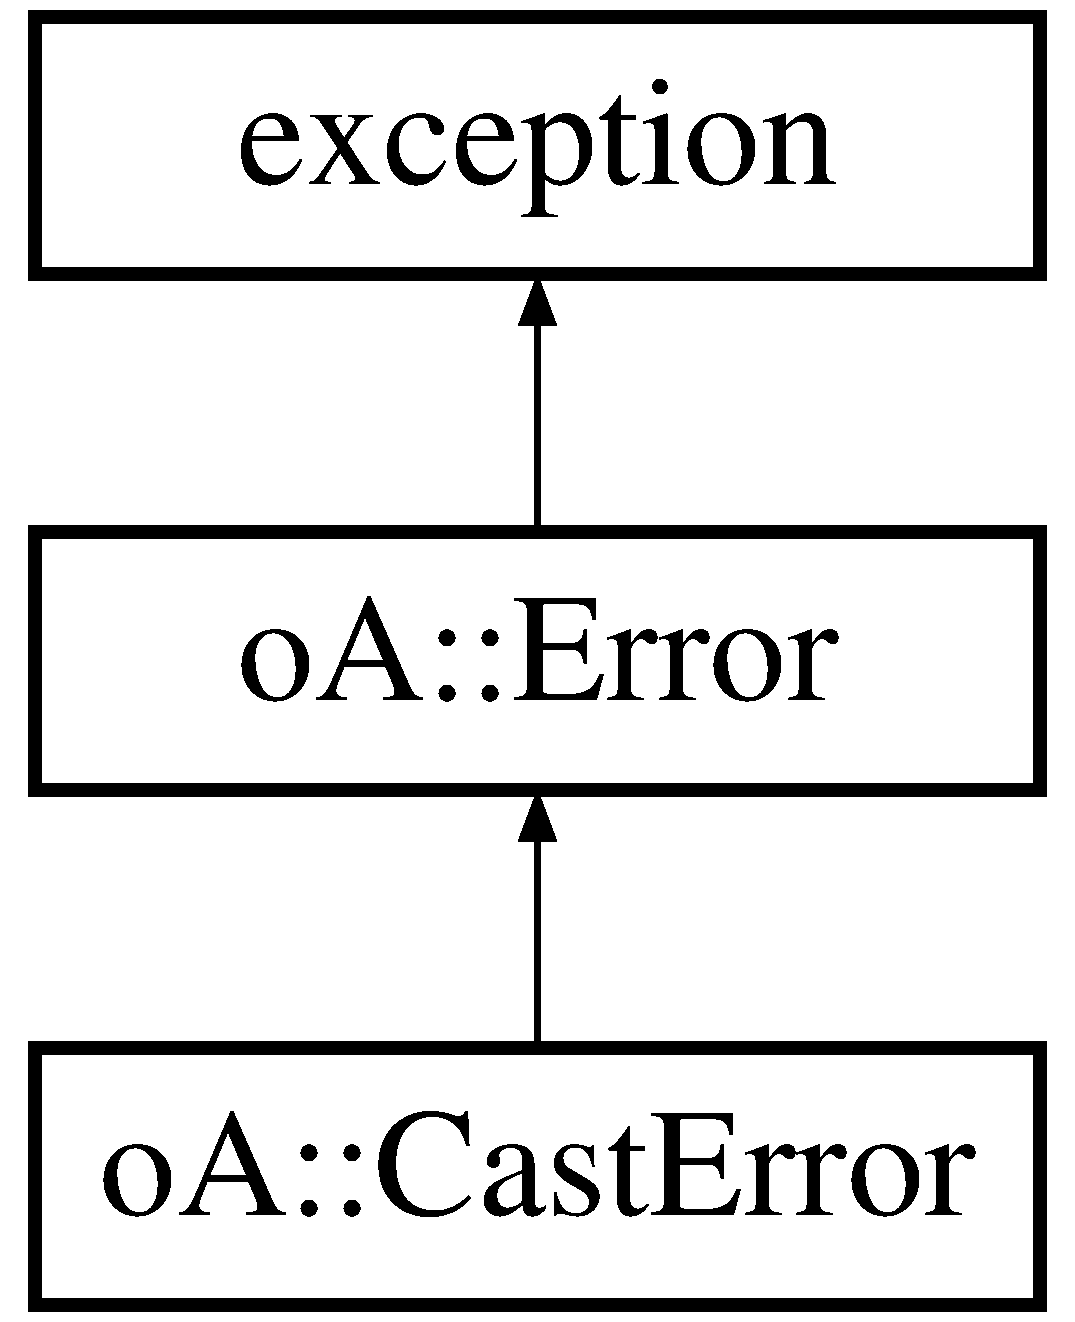
\includegraphics[height=3.000000cm]{classo_a_1_1_cast_error}
\end{center}
\end{figure}
\subsection*{Public Member Functions}
\begin{DoxyCompactItemize}
\item 
\mbox{\hyperlink{classo_a_1_1_cast_error_a16d10704561d2b756722d71d8703089c}{Error}} (const \mbox{\hyperlink{classo_a_1_1_string}{String}} \&msg)
\item 
\mbox{\hyperlink{classo_a_1_1_cast_error_adf66492ca8b03fa14d09e5bba7cdacbd}{Error}} (const \mbox{\hyperlink{classo_a_1_1_string}{String}} \&from, const \mbox{\hyperlink{classo_a_1_1_string}{String}} \&msg)
\end{DoxyCompactItemize}


\subsection{Member Function Documentation}
\mbox{\Hypertarget{classo_a_1_1_cast_error_a16d10704561d2b756722d71d8703089c}\label{classo_a_1_1_cast_error_a16d10704561d2b756722d71d8703089c}} 
\index{o\+A\+::\+Cast\+Error@{o\+A\+::\+Cast\+Error}!Error@{Error}}
\index{Error@{Error}!o\+A\+::\+Cast\+Error@{o\+A\+::\+Cast\+Error}}
\subsubsection{\texorpdfstring{Error()}{Error()}\hspace{0.1cm}{\footnotesize\ttfamily [1/2]}}
{\footnotesize\ttfamily o\+A\+::\+Error\+::\+Error\hspace{0.3cm}{\ttfamily [inline]}}

\mbox{\Hypertarget{classo_a_1_1_cast_error_adf66492ca8b03fa14d09e5bba7cdacbd}\label{classo_a_1_1_cast_error_adf66492ca8b03fa14d09e5bba7cdacbd}} 
\index{o\+A\+::\+Cast\+Error@{o\+A\+::\+Cast\+Error}!Error@{Error}}
\index{Error@{Error}!o\+A\+::\+Cast\+Error@{o\+A\+::\+Cast\+Error}}
\subsubsection{\texorpdfstring{Error()}{Error()}\hspace{0.1cm}{\footnotesize\ttfamily [2/2]}}
{\footnotesize\ttfamily o\+A\+::\+Error\+::\+Error\hspace{0.3cm}{\ttfamily [inline]}}



The documentation for this class was generated from the following file\+:\begin{DoxyCompactItemize}
\item 
Library/open\+App/\+Types/\mbox{\hyperlink{_error_8hpp}{Error.\+hpp}}\end{DoxyCompactItemize}

\hypertarget{classo_a_1_1_chrono}{}\section{oA\+:\+:Chrono Class Reference}
\label{classo_a_1_1_chrono}\index{o\+A\+::\+Chrono@{o\+A\+::\+Chrono}}


{\ttfamily \#include $<$Chrono.\+hpp$>$}

\subsection*{Public Member Functions}
\begin{DoxyCompactItemize}
\item 
\mbox{\hyperlink{classo_a_1_1_chrono_aec5a69450af4387e5d1b2b2344dc2bcd}{Chrono}} (void)
\item 
\mbox{\hyperlink{namespaceo_a_abe1d8250226c5cf34f84d7b75fc7922e}{Uint}} \mbox{\hyperlink{classo_a_1_1_chrono_a41692d0d58ca6cfc3570d1b2169b4a96}{get\+Seconds}} (void) const noexcept
\item 
\mbox{\hyperlink{namespaceo_a_abe1d8250226c5cf34f84d7b75fc7922e}{Uint}} \mbox{\hyperlink{classo_a_1_1_chrono_ad77117d4c523970030eda4cec93add7c}{get\+Milliseconds}} (void) const noexcept
\item 
\mbox{\hyperlink{namespaceo_a_abe1d8250226c5cf34f84d7b75fc7922e}{Uint}} \mbox{\hyperlink{classo_a_1_1_chrono_ac5ed210f5be9e507c95940356338bd88}{get\+Microseconds}} (void) const noexcept
\item 
void \mbox{\hyperlink{classo_a_1_1_chrono_a16943e5e5a0a768cd5b1a7af2deed739}{reset}} (void) noexcept
\item 
void \mbox{\hyperlink{classo_a_1_1_chrono_a64646924bdd219e72b58999745928fe6}{pause}} (void) noexcept
\item 
void \mbox{\hyperlink{classo_a_1_1_chrono_a2056863ec3fa0a94ed02fa0393b116e9}{resume}} (void) noexcept
\item 
bool \mbox{\hyperlink{classo_a_1_1_chrono_aeeaed136925a70bd668648b0a99b3f8e}{is\+Paused}} (void) const noexcept
\end{DoxyCompactItemize}


\subsection{Constructor \& Destructor Documentation}
\mbox{\Hypertarget{classo_a_1_1_chrono_aec5a69450af4387e5d1b2b2344dc2bcd}\label{classo_a_1_1_chrono_aec5a69450af4387e5d1b2b2344dc2bcd}} 
\index{o\+A\+::\+Chrono@{o\+A\+::\+Chrono}!Chrono@{Chrono}}
\index{Chrono@{Chrono}!o\+A\+::\+Chrono@{o\+A\+::\+Chrono}}
\subsubsection{\texorpdfstring{Chrono()}{Chrono()}}
{\footnotesize\ttfamily o\+A\+::\+Chrono\+::\+Chrono (\begin{DoxyParamCaption}\item[{void}]{ }\end{DoxyParamCaption})\hspace{0.3cm}{\ttfamily [inline]}}



\subsection{Member Function Documentation}
\mbox{\Hypertarget{classo_a_1_1_chrono_ac5ed210f5be9e507c95940356338bd88}\label{classo_a_1_1_chrono_ac5ed210f5be9e507c95940356338bd88}} 
\index{o\+A\+::\+Chrono@{o\+A\+::\+Chrono}!get\+Microseconds@{get\+Microseconds}}
\index{get\+Microseconds@{get\+Microseconds}!o\+A\+::\+Chrono@{o\+A\+::\+Chrono}}
\subsubsection{\texorpdfstring{get\+Microseconds()}{getMicroseconds()}}
{\footnotesize\ttfamily \mbox{\hyperlink{namespaceo_a_abe1d8250226c5cf34f84d7b75fc7922e}{Uint}} o\+A\+::\+Chrono\+::get\+Microseconds (\begin{DoxyParamCaption}\item[{void}]{ }\end{DoxyParamCaption}) const\hspace{0.3cm}{\ttfamily [inline]}, {\ttfamily [noexcept]}}

\mbox{\Hypertarget{classo_a_1_1_chrono_ad77117d4c523970030eda4cec93add7c}\label{classo_a_1_1_chrono_ad77117d4c523970030eda4cec93add7c}} 
\index{o\+A\+::\+Chrono@{o\+A\+::\+Chrono}!get\+Milliseconds@{get\+Milliseconds}}
\index{get\+Milliseconds@{get\+Milliseconds}!o\+A\+::\+Chrono@{o\+A\+::\+Chrono}}
\subsubsection{\texorpdfstring{get\+Milliseconds()}{getMilliseconds()}}
{\footnotesize\ttfamily \mbox{\hyperlink{namespaceo_a_abe1d8250226c5cf34f84d7b75fc7922e}{Uint}} o\+A\+::\+Chrono\+::get\+Milliseconds (\begin{DoxyParamCaption}\item[{void}]{ }\end{DoxyParamCaption}) const\hspace{0.3cm}{\ttfamily [inline]}, {\ttfamily [noexcept]}}

\mbox{\Hypertarget{classo_a_1_1_chrono_a41692d0d58ca6cfc3570d1b2169b4a96}\label{classo_a_1_1_chrono_a41692d0d58ca6cfc3570d1b2169b4a96}} 
\index{o\+A\+::\+Chrono@{o\+A\+::\+Chrono}!get\+Seconds@{get\+Seconds}}
\index{get\+Seconds@{get\+Seconds}!o\+A\+::\+Chrono@{o\+A\+::\+Chrono}}
\subsubsection{\texorpdfstring{get\+Seconds()}{getSeconds()}}
{\footnotesize\ttfamily \mbox{\hyperlink{namespaceo_a_abe1d8250226c5cf34f84d7b75fc7922e}{Uint}} o\+A\+::\+Chrono\+::get\+Seconds (\begin{DoxyParamCaption}\item[{void}]{ }\end{DoxyParamCaption}) const\hspace{0.3cm}{\ttfamily [inline]}, {\ttfamily [noexcept]}}

\mbox{\Hypertarget{classo_a_1_1_chrono_aeeaed136925a70bd668648b0a99b3f8e}\label{classo_a_1_1_chrono_aeeaed136925a70bd668648b0a99b3f8e}} 
\index{o\+A\+::\+Chrono@{o\+A\+::\+Chrono}!is\+Paused@{is\+Paused}}
\index{is\+Paused@{is\+Paused}!o\+A\+::\+Chrono@{o\+A\+::\+Chrono}}
\subsubsection{\texorpdfstring{is\+Paused()}{isPaused()}}
{\footnotesize\ttfamily bool o\+A\+::\+Chrono\+::is\+Paused (\begin{DoxyParamCaption}\item[{void}]{ }\end{DoxyParamCaption}) const\hspace{0.3cm}{\ttfamily [inline]}, {\ttfamily [noexcept]}}

\mbox{\Hypertarget{classo_a_1_1_chrono_a64646924bdd219e72b58999745928fe6}\label{classo_a_1_1_chrono_a64646924bdd219e72b58999745928fe6}} 
\index{o\+A\+::\+Chrono@{o\+A\+::\+Chrono}!pause@{pause}}
\index{pause@{pause}!o\+A\+::\+Chrono@{o\+A\+::\+Chrono}}
\subsubsection{\texorpdfstring{pause()}{pause()}}
{\footnotesize\ttfamily void o\+A\+::\+Chrono\+::pause (\begin{DoxyParamCaption}\item[{void}]{ }\end{DoxyParamCaption})\hspace{0.3cm}{\ttfamily [inline]}, {\ttfamily [noexcept]}}

\mbox{\Hypertarget{classo_a_1_1_chrono_a16943e5e5a0a768cd5b1a7af2deed739}\label{classo_a_1_1_chrono_a16943e5e5a0a768cd5b1a7af2deed739}} 
\index{o\+A\+::\+Chrono@{o\+A\+::\+Chrono}!reset@{reset}}
\index{reset@{reset}!o\+A\+::\+Chrono@{o\+A\+::\+Chrono}}
\subsubsection{\texorpdfstring{reset()}{reset()}}
{\footnotesize\ttfamily void o\+A\+::\+Chrono\+::reset (\begin{DoxyParamCaption}\item[{void}]{ }\end{DoxyParamCaption})\hspace{0.3cm}{\ttfamily [inline]}, {\ttfamily [noexcept]}}

\mbox{\Hypertarget{classo_a_1_1_chrono_a2056863ec3fa0a94ed02fa0393b116e9}\label{classo_a_1_1_chrono_a2056863ec3fa0a94ed02fa0393b116e9}} 
\index{o\+A\+::\+Chrono@{o\+A\+::\+Chrono}!resume@{resume}}
\index{resume@{resume}!o\+A\+::\+Chrono@{o\+A\+::\+Chrono}}
\subsubsection{\texorpdfstring{resume()}{resume()}}
{\footnotesize\ttfamily void o\+A\+::\+Chrono\+::resume (\begin{DoxyParamCaption}\item[{void}]{ }\end{DoxyParamCaption})\hspace{0.3cm}{\ttfamily [inline]}, {\ttfamily [noexcept]}}



The documentation for this class was generated from the following file\+:\begin{DoxyCompactItemize}
\item 
Library/open\+App/\+Core/\mbox{\hyperlink{_chrono_8hpp}{Chrono.\+hpp}}\end{DoxyCompactItemize}

\hypertarget{classo_a_1_1_color}{}\section{oA\+:\+:Color Class Reference}
\label{classo_a_1_1_color}\index{o\+A\+::\+Color@{o\+A\+::\+Color}}


Abstraction of a concatenated R\+G\+BA color.  




{\ttfamily \#include $<$Color.\+hpp$>$}

\subsection*{Public Member Functions}
\begin{DoxyCompactItemize}
\item 
\mbox{\hyperlink{classo_a_1_1_color_a62152f87069a3a2905086814012a3fea}{Color}} (\mbox{\hyperlink{namespaceo_a_a8c38e43a304d568b8495770dd8d50513}{U\+Byte}} r=0, \mbox{\hyperlink{namespaceo_a_a8c38e43a304d568b8495770dd8d50513}{U\+Byte}} g=0, \mbox{\hyperlink{namespaceo_a_a8c38e43a304d568b8495770dd8d50513}{U\+Byte}} b=0, \mbox{\hyperlink{namespaceo_a_a8c38e43a304d568b8495770dd8d50513}{U\+Byte}} a=255)
\begin{DoxyCompactList}\small\item\em Construct a new \mbox{\hyperlink{classo_a_1_1_color}{Color}} object. \end{DoxyCompactList}\item 
\mbox{\hyperlink{namespaceo_a_a8c38e43a304d568b8495770dd8d50513}{U\+Byte}} \mbox{\hyperlink{classo_a_1_1_color_a27cd67a64f4cc15f09fb7686890add8f}{getA}} (void) const noexcept
\begin{DoxyCompactList}\small\item\em Get alpha intensity. \end{DoxyCompactList}\item 
\mbox{\hyperlink{namespaceo_a_a8c38e43a304d568b8495770dd8d50513}{U\+Byte}} \mbox{\hyperlink{classo_a_1_1_color_af53e0f3c94638ab041fe05ce7356c2d8}{getR}} (void) const noexcept
\begin{DoxyCompactList}\small\item\em Get red intensity. \end{DoxyCompactList}\item 
\mbox{\hyperlink{namespaceo_a_a8c38e43a304d568b8495770dd8d50513}{U\+Byte}} \mbox{\hyperlink{classo_a_1_1_color_a3dcd5785db4a2c1a5a49a70d5378154a}{getG}} (void) const noexcept
\begin{DoxyCompactList}\small\item\em Get green intensity. \end{DoxyCompactList}\item 
\mbox{\hyperlink{namespaceo_a_a8c38e43a304d568b8495770dd8d50513}{U\+Byte}} \mbox{\hyperlink{classo_a_1_1_color_a8a30e79da1de484a4ff47ed2bcbc8e23}{getB}} (void) const noexcept
\begin{DoxyCompactList}\small\item\em Get blue intensity. \end{DoxyCompactList}\item 
\mbox{\hyperlink{namespaceo_a_abe1d8250226c5cf34f84d7b75fc7922e}{Uint}} \mbox{\hyperlink{classo_a_1_1_color_ac010d6318a14cebb3123929159fbab93}{get\+Value}} (void) const noexcept
\begin{DoxyCompactList}\small\item\em Get the internal concatened value. \end{DoxyCompactList}\item 
void \mbox{\hyperlink{classo_a_1_1_color_aaf0ba215d5bd4946f93a68bab2a8d66d}{set}} (\mbox{\hyperlink{namespaceo_a_a8c38e43a304d568b8495770dd8d50513}{U\+Byte}} r, \mbox{\hyperlink{namespaceo_a_a8c38e43a304d568b8495770dd8d50513}{U\+Byte}} g, \mbox{\hyperlink{namespaceo_a_a8c38e43a304d568b8495770dd8d50513}{U\+Byte}} b, \mbox{\hyperlink{namespaceo_a_a8c38e43a304d568b8495770dd8d50513}{U\+Byte}} a=255)
\begin{DoxyCompactList}\small\item\em Set a new concatened value. \end{DoxyCompactList}\item 
void \mbox{\hyperlink{classo_a_1_1_color_afa261cb70221d211e94a29b8f0484a02}{set\+Transparency}} (\mbox{\hyperlink{namespaceo_a_a8c38e43a304d568b8495770dd8d50513}{U\+Byte}} a)
\begin{DoxyCompactList}\small\item\em Set alpha intensity. \end{DoxyCompactList}\end{DoxyCompactItemize}
\subsection*{Static Public Member Functions}
\begin{DoxyCompactItemize}
\item 
static \mbox{\hyperlink{classo_a_1_1_color}{Color}} \mbox{\hyperlink{classo_a_1_1_color_ae637744de31ea0e978b58a836db49884}{Retreive\+Color}} (const \mbox{\hyperlink{classo_a_1_1_string}{String}} \&color)
\begin{DoxyCompactList}\small\item\em Retreive a color using a \#\+String identifier. \end{DoxyCompactList}\end{DoxyCompactItemize}


\subsection{Detailed Description}
Abstraction of a concatenated R\+G\+BA color. 

Note that the internal value is A.\+R.\+G.\+B shifted in a single \mbox{\hyperlink{namespaceo_a_abe1d8250226c5cf34f84d7b75fc7922e}{Uint}} 

\subsection{Constructor \& Destructor Documentation}
\mbox{\Hypertarget{classo_a_1_1_color_a62152f87069a3a2905086814012a3fea}\label{classo_a_1_1_color_a62152f87069a3a2905086814012a3fea}} 
\index{o\+A\+::\+Color@{o\+A\+::\+Color}!Color@{Color}}
\index{Color@{Color}!o\+A\+::\+Color@{o\+A\+::\+Color}}
\subsubsection{\texorpdfstring{Color()}{Color()}}
{\footnotesize\ttfamily o\+A\+::\+Color\+::\+Color (\begin{DoxyParamCaption}\item[{\mbox{\hyperlink{namespaceo_a_a8c38e43a304d568b8495770dd8d50513}{U\+Byte}}}]{r = {\ttfamily 0},  }\item[{\mbox{\hyperlink{namespaceo_a_a8c38e43a304d568b8495770dd8d50513}{U\+Byte}}}]{g = {\ttfamily 0},  }\item[{\mbox{\hyperlink{namespaceo_a_a8c38e43a304d568b8495770dd8d50513}{U\+Byte}}}]{b = {\ttfamily 0},  }\item[{\mbox{\hyperlink{namespaceo_a_a8c38e43a304d568b8495770dd8d50513}{U\+Byte}}}]{a = {\ttfamily 255} }\end{DoxyParamCaption})\hspace{0.3cm}{\ttfamily [inline]}}



Construct a new \mbox{\hyperlink{classo_a_1_1_color}{Color}} object. 


\begin{DoxyParams}{Parameters}
{\em r} & Red intensity \\
\hline
{\em g} & Green intensity \\
\hline
{\em b} & Blue intensity \\
\hline
{\em a} & Alpha intensity \\
\hline
\end{DoxyParams}


\subsection{Member Function Documentation}
\mbox{\Hypertarget{classo_a_1_1_color_a27cd67a64f4cc15f09fb7686890add8f}\label{classo_a_1_1_color_a27cd67a64f4cc15f09fb7686890add8f}} 
\index{o\+A\+::\+Color@{o\+A\+::\+Color}!getA@{getA}}
\index{getA@{getA}!o\+A\+::\+Color@{o\+A\+::\+Color}}
\subsubsection{\texorpdfstring{get\+A()}{getA()}}
{\footnotesize\ttfamily \mbox{\hyperlink{namespaceo_a_a8c38e43a304d568b8495770dd8d50513}{U\+Byte}} o\+A\+::\+Color\+::getA (\begin{DoxyParamCaption}\item[{void}]{ }\end{DoxyParamCaption}) const\hspace{0.3cm}{\ttfamily [inline]}, {\ttfamily [noexcept]}}



Get alpha intensity. 

\begin{DoxyReturn}{Returns}
U\+Byte Alpha intensity 
\end{DoxyReturn}
\mbox{\Hypertarget{classo_a_1_1_color_a8a30e79da1de484a4ff47ed2bcbc8e23}\label{classo_a_1_1_color_a8a30e79da1de484a4ff47ed2bcbc8e23}} 
\index{o\+A\+::\+Color@{o\+A\+::\+Color}!getB@{getB}}
\index{getB@{getB}!o\+A\+::\+Color@{o\+A\+::\+Color}}
\subsubsection{\texorpdfstring{get\+B()}{getB()}}
{\footnotesize\ttfamily \mbox{\hyperlink{namespaceo_a_a8c38e43a304d568b8495770dd8d50513}{U\+Byte}} o\+A\+::\+Color\+::getB (\begin{DoxyParamCaption}\item[{void}]{ }\end{DoxyParamCaption}) const\hspace{0.3cm}{\ttfamily [inline]}, {\ttfamily [noexcept]}}



Get blue intensity. 

\begin{DoxyReturn}{Returns}
U\+Byte Blue intensity 
\end{DoxyReturn}
\mbox{\Hypertarget{classo_a_1_1_color_a3dcd5785db4a2c1a5a49a70d5378154a}\label{classo_a_1_1_color_a3dcd5785db4a2c1a5a49a70d5378154a}} 
\index{o\+A\+::\+Color@{o\+A\+::\+Color}!getG@{getG}}
\index{getG@{getG}!o\+A\+::\+Color@{o\+A\+::\+Color}}
\subsubsection{\texorpdfstring{get\+G()}{getG()}}
{\footnotesize\ttfamily \mbox{\hyperlink{namespaceo_a_a8c38e43a304d568b8495770dd8d50513}{U\+Byte}} o\+A\+::\+Color\+::getG (\begin{DoxyParamCaption}\item[{void}]{ }\end{DoxyParamCaption}) const\hspace{0.3cm}{\ttfamily [inline]}, {\ttfamily [noexcept]}}



Get green intensity. 

\begin{DoxyReturn}{Returns}
U\+Byte Green intensity 
\end{DoxyReturn}
\mbox{\Hypertarget{classo_a_1_1_color_af53e0f3c94638ab041fe05ce7356c2d8}\label{classo_a_1_1_color_af53e0f3c94638ab041fe05ce7356c2d8}} 
\index{o\+A\+::\+Color@{o\+A\+::\+Color}!getR@{getR}}
\index{getR@{getR}!o\+A\+::\+Color@{o\+A\+::\+Color}}
\subsubsection{\texorpdfstring{get\+R()}{getR()}}
{\footnotesize\ttfamily \mbox{\hyperlink{namespaceo_a_a8c38e43a304d568b8495770dd8d50513}{U\+Byte}} o\+A\+::\+Color\+::getR (\begin{DoxyParamCaption}\item[{void}]{ }\end{DoxyParamCaption}) const\hspace{0.3cm}{\ttfamily [inline]}, {\ttfamily [noexcept]}}



Get red intensity. 

\begin{DoxyReturn}{Returns}
U\+Byte Red intensity 
\end{DoxyReturn}
\mbox{\Hypertarget{classo_a_1_1_color_ac010d6318a14cebb3123929159fbab93}\label{classo_a_1_1_color_ac010d6318a14cebb3123929159fbab93}} 
\index{o\+A\+::\+Color@{o\+A\+::\+Color}!get\+Value@{get\+Value}}
\index{get\+Value@{get\+Value}!o\+A\+::\+Color@{o\+A\+::\+Color}}
\subsubsection{\texorpdfstring{get\+Value()}{getValue()}}
{\footnotesize\ttfamily \mbox{\hyperlink{namespaceo_a_abe1d8250226c5cf34f84d7b75fc7922e}{Uint}} o\+A\+::\+Color\+::get\+Value (\begin{DoxyParamCaption}\item[{void}]{ }\end{DoxyParamCaption}) const\hspace{0.3cm}{\ttfamily [inline]}, {\ttfamily [noexcept]}}



Get the internal concatened value. 

\begin{DoxyReturn}{Returns}
Uint Concatenated value 
\end{DoxyReturn}
\mbox{\Hypertarget{classo_a_1_1_color_ae637744de31ea0e978b58a836db49884}\label{classo_a_1_1_color_ae637744de31ea0e978b58a836db49884}} 
\index{o\+A\+::\+Color@{o\+A\+::\+Color}!Retreive\+Color@{Retreive\+Color}}
\index{Retreive\+Color@{Retreive\+Color}!o\+A\+::\+Color@{o\+A\+::\+Color}}
\subsubsection{\texorpdfstring{Retreive\+Color()}{RetreiveColor()}}
{\footnotesize\ttfamily \mbox{\hyperlink{classo_a_1_1_color}{o\+A\+::\+Color}} o\+A\+::\+Color\+::\+Retreive\+Color (\begin{DoxyParamCaption}\item[{const \mbox{\hyperlink{classo_a_1_1_string}{String}} \&}]{color }\end{DoxyParamCaption})\hspace{0.3cm}{\ttfamily [static]}}



Retreive a color using a \#\+String identifier. 


\begin{DoxyParams}{Parameters}
{\em color} & Identifier \\
\hline
\end{DoxyParams}
\begin{DoxyReturn}{Returns}
\mbox{\hyperlink{classo_a_1_1_color}{Color}} Identified color 
\end{DoxyReturn}
\mbox{\Hypertarget{classo_a_1_1_color_aaf0ba215d5bd4946f93a68bab2a8d66d}\label{classo_a_1_1_color_aaf0ba215d5bd4946f93a68bab2a8d66d}} 
\index{o\+A\+::\+Color@{o\+A\+::\+Color}!set@{set}}
\index{set@{set}!o\+A\+::\+Color@{o\+A\+::\+Color}}
\subsubsection{\texorpdfstring{set()}{set()}}
{\footnotesize\ttfamily void o\+A\+::\+Color\+::set (\begin{DoxyParamCaption}\item[{\mbox{\hyperlink{namespaceo_a_a8c38e43a304d568b8495770dd8d50513}{U\+Byte}}}]{r,  }\item[{\mbox{\hyperlink{namespaceo_a_a8c38e43a304d568b8495770dd8d50513}{U\+Byte}}}]{g,  }\item[{\mbox{\hyperlink{namespaceo_a_a8c38e43a304d568b8495770dd8d50513}{U\+Byte}}}]{b,  }\item[{\mbox{\hyperlink{namespaceo_a_a8c38e43a304d568b8495770dd8d50513}{U\+Byte}}}]{a = {\ttfamily 255} }\end{DoxyParamCaption})}



Set a new concatened value. 


\begin{DoxyParams}{Parameters}
{\em r} & Red intensity \\
\hline
{\em g} & Green intensity \\
\hline
{\em b} & Blue intensity \\
\hline
{\em a} & Alpha intensity \\
\hline
\end{DoxyParams}
\mbox{\Hypertarget{classo_a_1_1_color_afa261cb70221d211e94a29b8f0484a02}\label{classo_a_1_1_color_afa261cb70221d211e94a29b8f0484a02}} 
\index{o\+A\+::\+Color@{o\+A\+::\+Color}!set\+Transparency@{set\+Transparency}}
\index{set\+Transparency@{set\+Transparency}!o\+A\+::\+Color@{o\+A\+::\+Color}}
\subsubsection{\texorpdfstring{set\+Transparency()}{setTransparency()}}
{\footnotesize\ttfamily void o\+A\+::\+Color\+::set\+Transparency (\begin{DoxyParamCaption}\item[{\mbox{\hyperlink{namespaceo_a_a8c38e43a304d568b8495770dd8d50513}{U\+Byte}}}]{a }\end{DoxyParamCaption})}



Set alpha intensity. 


\begin{DoxyParams}{Parameters}
{\em a} & Alpha intensity \\
\hline
\end{DoxyParams}


The documentation for this class was generated from the following files\+:\begin{DoxyCompactItemize}
\item 
Library/open\+App/\+Types/\mbox{\hyperlink{_color_8hpp}{Color.\+hpp}}\item 
Library/open\+App/\+Types/\mbox{\hyperlink{_color_8cpp}{Color.\+cpp}}\end{DoxyCompactItemize}

\hypertarget{classo_a_1_1_container_helper}{}\section{oA\+:\+:Container\+Helper$<$ Container\+Type, Value $>$ Class Template Reference}
\label{classo_a_1_1_container_helper}\index{o\+A\+::\+Container\+Helper$<$ Container\+Type, Value $>$@{o\+A\+::\+Container\+Helper$<$ Container\+Type, Value $>$}}


Standard container extender.  




{\ttfamily \#include $<$Container\+Helper.\+hpp$>$}

Inheritance diagram for oA\+:\+:Container\+Helper$<$ Container\+Type, Value $>$\+:\begin{figure}[H]
\begin{center}
\leavevmode
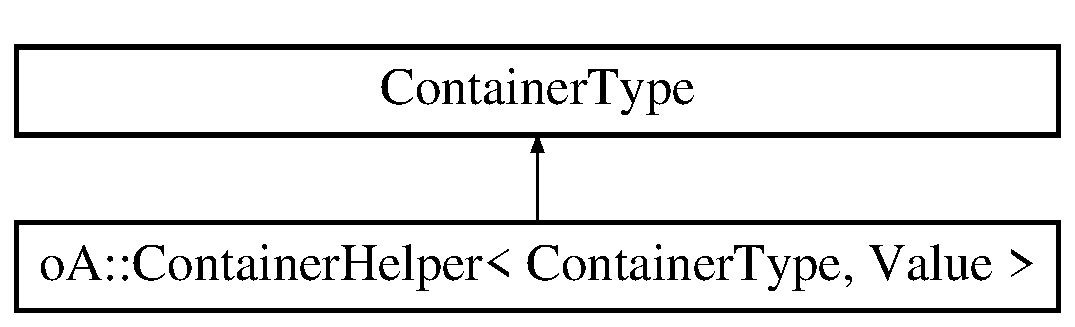
\includegraphics[height=2.000000cm]{classo_a_1_1_container_helper}
\end{center}
\end{figure}
\subsection*{Public Member Functions}
\begin{DoxyCompactItemize}
\item 
{\footnotesize template$<$typename Signature $>$ }\\void \mbox{\hyperlink{classo_a_1_1_container_helper_ab0a8a0bce2178cf1ded50b3d4202aa39}{apply}} (const Signature \&fct)
\begin{DoxyCompactList}\small\item\em Apply a non-\/const function to every element. \end{DoxyCompactList}\item 
{\footnotesize template$<$typename Signature $>$ }\\void \mbox{\hyperlink{classo_a_1_1_container_helper_a659bf470905acc97ae8badf9e985190b}{apply}} (const Signature \&fct) const
\begin{DoxyCompactList}\small\item\em Apply a const function to every element. \end{DoxyCompactList}\item 
void \mbox{\hyperlink{classo_a_1_1_container_helper_a9ed895ce074880a44d19c0b37da02c83}{remove\+If}} (const Value \&to\+Remove)
\begin{DoxyCompactList}\small\item\em Remove every element matching a value. \end{DoxyCompactList}\item 
{\footnotesize template$<$typename Signature $>$ }\\void \mbox{\hyperlink{classo_a_1_1_container_helper_abeca65c6bc826fe9ad640599a8912dc3}{remove\+If}} (const Signature \&predicate)
\begin{DoxyCompactList}\small\item\em Remove every elements matching a predicate. \end{DoxyCompactList}\item 
{\footnotesize template$<$typename Signature $>$ }\\auto \mbox{\hyperlink{classo_a_1_1_container_helper_af2ed8bdecb2d870ba366ee56d7e6b90a}{find\+If}} (const Signature \&predicate)
\begin{DoxyCompactList}\small\item\em Retreive the first non-\/const element matching the predicate. \end{DoxyCompactList}\item 
{\footnotesize template$<$typename Signature $>$ }\\auto \mbox{\hyperlink{classo_a_1_1_container_helper_accea76cd23603fc42db7b46081f5cc8d}{find\+If}} (const Signature \&predicate) const
\begin{DoxyCompactList}\small\item\em Retreive the first const element matching the predicate. \end{DoxyCompactList}\item 
{\footnotesize template$<$typename Iterator , typename Signature $>$ }\\auto \mbox{\hyperlink{classo_a_1_1_container_helper_a65c48f0a1d310ae5bb9d1f04509cf0ff}{find\+If}} (Iterator start, const Signature \&predicate)
\begin{DoxyCompactList}\small\item\em Retreive the first non-\/const element matching the predicate, starting at given iterator. \end{DoxyCompactList}\item 
{\footnotesize template$<$typename Iterator , typename Signature $>$ }\\auto \mbox{\hyperlink{classo_a_1_1_container_helper_a7fdcb06a5193933448ec214640501705}{find\+If}} (Iterator start, const Signature \&predicate) const
\begin{DoxyCompactList}\small\item\em Retreive the first const element matching the predicate, starting at given iterator. \end{DoxyCompactList}\end{DoxyCompactItemize}


\subsection{Detailed Description}
\subsubsection*{template$<$typename Container\+Type, typename Value$>$\newline
class o\+A\+::\+Container\+Helper$<$ Container\+Type, Value $>$}

Standard container extender. 


\begin{DoxyTemplParams}{Template Parameters}
{\em Container\+Type} & Type of the container \\
\hline
{\em Value} & Value of Type\textquotesingle{}s container \\
\hline
\end{DoxyTemplParams}


\subsection{Member Function Documentation}
\mbox{\Hypertarget{classo_a_1_1_container_helper_ab0a8a0bce2178cf1ded50b3d4202aa39}\label{classo_a_1_1_container_helper_ab0a8a0bce2178cf1ded50b3d4202aa39}} 
\index{o\+A\+::\+Container\+Helper@{o\+A\+::\+Container\+Helper}!apply@{apply}}
\index{apply@{apply}!o\+A\+::\+Container\+Helper@{o\+A\+::\+Container\+Helper}}
\subsubsection{\texorpdfstring{apply()}{apply()}\hspace{0.1cm}{\footnotesize\ttfamily [1/2]}}
{\footnotesize\ttfamily template$<$typename Container\+Type, typename Value$>$ \\
template$<$typename Signature $>$ \\
void \mbox{\hyperlink{classo_a_1_1_container_helper}{o\+A\+::\+Container\+Helper}}$<$ Container\+Type, Value $>$\+::apply (\begin{DoxyParamCaption}\item[{const Signature \&}]{fct }\end{DoxyParamCaption})\hspace{0.3cm}{\ttfamily [inline]}}



Apply a non-\/const function to every element. 


\begin{DoxyTemplParams}{Template Parameters}
{\em Signature} & Applied function signature \\
\hline
\end{DoxyTemplParams}

\begin{DoxyParams}{Parameters}
{\em fct} & Applied function \\
\hline
\end{DoxyParams}
\mbox{\Hypertarget{classo_a_1_1_container_helper_a659bf470905acc97ae8badf9e985190b}\label{classo_a_1_1_container_helper_a659bf470905acc97ae8badf9e985190b}} 
\index{o\+A\+::\+Container\+Helper@{o\+A\+::\+Container\+Helper}!apply@{apply}}
\index{apply@{apply}!o\+A\+::\+Container\+Helper@{o\+A\+::\+Container\+Helper}}
\subsubsection{\texorpdfstring{apply()}{apply()}\hspace{0.1cm}{\footnotesize\ttfamily [2/2]}}
{\footnotesize\ttfamily template$<$typename Container\+Type, typename Value$>$ \\
template$<$typename Signature $>$ \\
void \mbox{\hyperlink{classo_a_1_1_container_helper}{o\+A\+::\+Container\+Helper}}$<$ Container\+Type, Value $>$\+::apply (\begin{DoxyParamCaption}\item[{const Signature \&}]{fct }\end{DoxyParamCaption}) const\hspace{0.3cm}{\ttfamily [inline]}}



Apply a const function to every element. 


\begin{DoxyTemplParams}{Template Parameters}
{\em Signature} & Applied function signature \\
\hline
\end{DoxyTemplParams}

\begin{DoxyParams}{Parameters}
{\em fct} & Applied function \\
\hline
\end{DoxyParams}
\mbox{\Hypertarget{classo_a_1_1_container_helper_af2ed8bdecb2d870ba366ee56d7e6b90a}\label{classo_a_1_1_container_helper_af2ed8bdecb2d870ba366ee56d7e6b90a}} 
\index{o\+A\+::\+Container\+Helper@{o\+A\+::\+Container\+Helper}!find\+If@{find\+If}}
\index{find\+If@{find\+If}!o\+A\+::\+Container\+Helper@{o\+A\+::\+Container\+Helper}}
\subsubsection{\texorpdfstring{find\+If()}{findIf()}\hspace{0.1cm}{\footnotesize\ttfamily [1/4]}}
{\footnotesize\ttfamily template$<$typename Container\+Type, typename Value$>$ \\
template$<$typename Signature $>$ \\
auto \mbox{\hyperlink{classo_a_1_1_container_helper}{o\+A\+::\+Container\+Helper}}$<$ Container\+Type, Value $>$\+::find\+If (\begin{DoxyParamCaption}\item[{const Signature \&}]{predicate }\end{DoxyParamCaption})\hspace{0.3cm}{\ttfamily [inline]}}



Retreive the first non-\/const element matching the predicate. 


\begin{DoxyTemplParams}{Template Parameters}
{\em Signature} & Predicate signature \\
\hline
\end{DoxyTemplParams}

\begin{DoxyParams}{Parameters}
{\em predicate} & Match function (must return a boolean) \\
\hline
\end{DoxyParams}
\mbox{\Hypertarget{classo_a_1_1_container_helper_accea76cd23603fc42db7b46081f5cc8d}\label{classo_a_1_1_container_helper_accea76cd23603fc42db7b46081f5cc8d}} 
\index{o\+A\+::\+Container\+Helper@{o\+A\+::\+Container\+Helper}!find\+If@{find\+If}}
\index{find\+If@{find\+If}!o\+A\+::\+Container\+Helper@{o\+A\+::\+Container\+Helper}}
\subsubsection{\texorpdfstring{find\+If()}{findIf()}\hspace{0.1cm}{\footnotesize\ttfamily [2/4]}}
{\footnotesize\ttfamily template$<$typename Container\+Type, typename Value$>$ \\
template$<$typename Signature $>$ \\
auto \mbox{\hyperlink{classo_a_1_1_container_helper}{o\+A\+::\+Container\+Helper}}$<$ Container\+Type, Value $>$\+::find\+If (\begin{DoxyParamCaption}\item[{const Signature \&}]{predicate }\end{DoxyParamCaption}) const\hspace{0.3cm}{\ttfamily [inline]}}



Retreive the first const element matching the predicate. 


\begin{DoxyTemplParams}{Template Parameters}
{\em Signature} & Predicate signature \\
\hline
\end{DoxyTemplParams}

\begin{DoxyParams}{Parameters}
{\em predicate} & Match function (must return a boolean) \\
\hline
\end{DoxyParams}
\mbox{\Hypertarget{classo_a_1_1_container_helper_a65c48f0a1d310ae5bb9d1f04509cf0ff}\label{classo_a_1_1_container_helper_a65c48f0a1d310ae5bb9d1f04509cf0ff}} 
\index{o\+A\+::\+Container\+Helper@{o\+A\+::\+Container\+Helper}!find\+If@{find\+If}}
\index{find\+If@{find\+If}!o\+A\+::\+Container\+Helper@{o\+A\+::\+Container\+Helper}}
\subsubsection{\texorpdfstring{find\+If()}{findIf()}\hspace{0.1cm}{\footnotesize\ttfamily [3/4]}}
{\footnotesize\ttfamily template$<$typename Container\+Type, typename Value$>$ \\
template$<$typename Iterator , typename Signature $>$ \\
auto \mbox{\hyperlink{classo_a_1_1_container_helper}{o\+A\+::\+Container\+Helper}}$<$ Container\+Type, Value $>$\+::find\+If (\begin{DoxyParamCaption}\item[{Iterator}]{start,  }\item[{const Signature \&}]{predicate }\end{DoxyParamCaption})\hspace{0.3cm}{\ttfamily [inline]}}



Retreive the first non-\/const element matching the predicate, starting at given iterator. 


\begin{DoxyTemplParams}{Template Parameters}
{\em Iterator} & Iterator type \\
\hline
{\em Signature} & Predication signature \\
\hline
\end{DoxyTemplParams}

\begin{DoxyParams}{Parameters}
{\em start} & Begin of search interator \\
\hline
{\em predicate} & Match function (must return a boolean) \\
\hline
\end{DoxyParams}
\begin{DoxyReturn}{Returns}
Iterator Matching iterator if found 
\end{DoxyReturn}
\mbox{\Hypertarget{classo_a_1_1_container_helper_a7fdcb06a5193933448ec214640501705}\label{classo_a_1_1_container_helper_a7fdcb06a5193933448ec214640501705}} 
\index{o\+A\+::\+Container\+Helper@{o\+A\+::\+Container\+Helper}!find\+If@{find\+If}}
\index{find\+If@{find\+If}!o\+A\+::\+Container\+Helper@{o\+A\+::\+Container\+Helper}}
\subsubsection{\texorpdfstring{find\+If()}{findIf()}\hspace{0.1cm}{\footnotesize\ttfamily [4/4]}}
{\footnotesize\ttfamily template$<$typename Container\+Type, typename Value$>$ \\
template$<$typename Iterator , typename Signature $>$ \\
auto \mbox{\hyperlink{classo_a_1_1_container_helper}{o\+A\+::\+Container\+Helper}}$<$ Container\+Type, Value $>$\+::find\+If (\begin{DoxyParamCaption}\item[{Iterator}]{start,  }\item[{const Signature \&}]{predicate }\end{DoxyParamCaption}) const\hspace{0.3cm}{\ttfamily [inline]}}



Retreive the first const element matching the predicate, starting at given iterator. 


\begin{DoxyTemplParams}{Template Parameters}
{\em Iterator} & Iterator type \\
\hline
{\em Signature} & Predication signature \\
\hline
\end{DoxyTemplParams}

\begin{DoxyParams}{Parameters}
{\em start} & Begin of search interator \\
\hline
{\em predicate} & Match function (must return a boolean) \\
\hline
\end{DoxyParams}
\begin{DoxyReturn}{Returns}
Iterator Matching iterator if found 
\end{DoxyReturn}
\mbox{\Hypertarget{classo_a_1_1_container_helper_a9ed895ce074880a44d19c0b37da02c83}\label{classo_a_1_1_container_helper_a9ed895ce074880a44d19c0b37da02c83}} 
\index{o\+A\+::\+Container\+Helper@{o\+A\+::\+Container\+Helper}!remove\+If@{remove\+If}}
\index{remove\+If@{remove\+If}!o\+A\+::\+Container\+Helper@{o\+A\+::\+Container\+Helper}}
\subsubsection{\texorpdfstring{remove\+If()}{removeIf()}\hspace{0.1cm}{\footnotesize\ttfamily [1/2]}}
{\footnotesize\ttfamily template$<$typename Container\+Type, typename Value$>$ \\
void \mbox{\hyperlink{classo_a_1_1_container_helper}{o\+A\+::\+Container\+Helper}}$<$ Container\+Type, Value $>$\+::remove\+If (\begin{DoxyParamCaption}\item[{const Value \&}]{to\+Remove }\end{DoxyParamCaption})\hspace{0.3cm}{\ttfamily [inline]}}



Remove every element matching a value. 


\begin{DoxyParams}{Parameters}
{\em to\+Remove} & Matching value to remove \\
\hline
\end{DoxyParams}
\mbox{\Hypertarget{classo_a_1_1_container_helper_abeca65c6bc826fe9ad640599a8912dc3}\label{classo_a_1_1_container_helper_abeca65c6bc826fe9ad640599a8912dc3}} 
\index{o\+A\+::\+Container\+Helper@{o\+A\+::\+Container\+Helper}!remove\+If@{remove\+If}}
\index{remove\+If@{remove\+If}!o\+A\+::\+Container\+Helper@{o\+A\+::\+Container\+Helper}}
\subsubsection{\texorpdfstring{remove\+If()}{removeIf()}\hspace{0.1cm}{\footnotesize\ttfamily [2/2]}}
{\footnotesize\ttfamily template$<$typename Container\+Type, typename Value$>$ \\
template$<$typename Signature $>$ \\
void \mbox{\hyperlink{classo_a_1_1_container_helper}{o\+A\+::\+Container\+Helper}}$<$ Container\+Type, Value $>$\+::remove\+If (\begin{DoxyParamCaption}\item[{const Signature \&}]{predicate }\end{DoxyParamCaption})\hspace{0.3cm}{\ttfamily [inline]}}



Remove every elements matching a predicate. 


\begin{DoxyTemplParams}{Template Parameters}
{\em Signature} & Predicate signature \\
\hline
\end{DoxyTemplParams}

\begin{DoxyParams}{Parameters}
{\em predicate} & Match function (must return a boolean) \\
\hline
\end{DoxyParams}


The documentation for this class was generated from the following file\+:\begin{DoxyCompactItemize}
\item 
Library/open\+App/\+Containers/\mbox{\hyperlink{_container_helper_8hpp}{Container\+Helper.\+hpp}}\end{DoxyCompactItemize}

\hypertarget{classo_a_1_1_endl}{}\section{oA\+:\+:Endl Class Reference}
\label{classo_a_1_1_endl}\index{o\+A\+::\+Endl@{o\+A\+::\+Endl}}


\mbox{\hyperlink{classo_a_1_1_endl}{Endl}} is used to insert a newline and flush into a \#\+Log.  




{\ttfamily \#include $<$Log\+Utils.\+hpp$>$}



\subsection{Detailed Description}
\mbox{\hyperlink{classo_a_1_1_endl}{Endl}} is used to insert a newline and flush into a \#\+Log. 

The documentation for this class was generated from the following file\+:\begin{DoxyCompactItemize}
\item 
Library/open\+App/\+Core/\mbox{\hyperlink{_log_utils_8hpp}{Log\+Utils.\+hpp}}\end{DoxyCompactItemize}

\hypertarget{classo_a_1_1_error}{}\section{oA\+:\+:Error Class Reference}
\label{classo_a_1_1_error}\index{o\+A\+::\+Error@{o\+A\+::\+Error}}


\mbox{\hyperlink{classo_a_1_1_error}{Error}} exception base.  




{\ttfamily \#include $<$Error.\+hpp$>$}



Inheritance diagram for oA\+:\+:Error\+:
% FIG 0


Collaboration diagram for oA\+:\+:Error\+:
% FIG 1
\subsection*{Public Member Functions}
\begin{DoxyCompactItemize}
\item 
\mbox{\hyperlink{classo_a_1_1_error_a16d10704561d2b756722d71d8703089c}{Error}} (const \mbox{\hyperlink{classo_a_1_1_string}{String}} \&msg)
\begin{DoxyCompactList}\small\item\em Construct a new \mbox{\hyperlink{classo_a_1_1_error}{Error}} object with an error message. \end{DoxyCompactList}\item 
\mbox{\hyperlink{classo_a_1_1_error_adf66492ca8b03fa14d09e5bba7cdacbd}{Error}} (const \mbox{\hyperlink{classo_a_1_1_string}{String}} \&from, const \mbox{\hyperlink{classo_a_1_1_string}{String}} \&msg)
\begin{DoxyCompactList}\small\item\em Construct a new \mbox{\hyperlink{classo_a_1_1_error}{Error}} object with a quoted source and an error message. \end{DoxyCompactList}\item 
virtual const char $\ast$ \mbox{\hyperlink{classo_a_1_1_error_aaef80480c87b91b1a34853c791b649ef}{what}} (void) const noexcept
\begin{DoxyCompactList}\small\item\em Return internal message. \end{DoxyCompactList}\end{DoxyCompactItemize}


\subsection{Detailed Description}
\mbox{\hyperlink{classo_a_1_1_error}{Error}} exception base. 

\subsection{Constructor \& Destructor Documentation}
\mbox{\Hypertarget{classo_a_1_1_error_a16d10704561d2b756722d71d8703089c}\label{classo_a_1_1_error_a16d10704561d2b756722d71d8703089c}} 
\index{o\+A\+::\+Error@{o\+A\+::\+Error}!Error@{Error}}
\index{Error@{Error}!o\+A\+::\+Error@{o\+A\+::\+Error}}
\subsubsection{\texorpdfstring{Error()}{Error()}\hspace{0.1cm}{\footnotesize\ttfamily [1/2]}}
{\footnotesize\ttfamily o\+A\+::\+Error\+::\+Error (\begin{DoxyParamCaption}\item[{const \mbox{\hyperlink{classo_a_1_1_string}{String}} \&}]{msg }\end{DoxyParamCaption})\hspace{0.3cm}{\ttfamily [inline]}}



Construct a new \mbox{\hyperlink{classo_a_1_1_error}{Error}} object with an error message. 


\begin{DoxyParams}{Parameters}
{\em msg} & \mbox{\hyperlink{classo_a_1_1_error}{Error}} message \\
\hline
\end{DoxyParams}
\mbox{\Hypertarget{classo_a_1_1_error_adf66492ca8b03fa14d09e5bba7cdacbd}\label{classo_a_1_1_error_adf66492ca8b03fa14d09e5bba7cdacbd}} 
\index{o\+A\+::\+Error@{o\+A\+::\+Error}!Error@{Error}}
\index{Error@{Error}!o\+A\+::\+Error@{o\+A\+::\+Error}}
\subsubsection{\texorpdfstring{Error()}{Error()}\hspace{0.1cm}{\footnotesize\ttfamily [2/2]}}
{\footnotesize\ttfamily o\+A\+::\+Error\+::\+Error (\begin{DoxyParamCaption}\item[{const \mbox{\hyperlink{classo_a_1_1_string}{String}} \&}]{from,  }\item[{const \mbox{\hyperlink{classo_a_1_1_string}{String}} \&}]{msg }\end{DoxyParamCaption})\hspace{0.3cm}{\ttfamily [inline]}}



Construct a new \mbox{\hyperlink{classo_a_1_1_error}{Error}} object with a quoted source and an error message. 


\begin{DoxyParams}{Parameters}
{\em from} & Source \\
\hline
{\em msg} & \mbox{\hyperlink{classo_a_1_1_error}{Error}} message \\
\hline
\end{DoxyParams}


\subsection{Member Function Documentation}
\mbox{\Hypertarget{classo_a_1_1_error_aaef80480c87b91b1a34853c791b649ef}\label{classo_a_1_1_error_aaef80480c87b91b1a34853c791b649ef}} 
\index{o\+A\+::\+Error@{o\+A\+::\+Error}!what@{what}}
\index{what@{what}!o\+A\+::\+Error@{o\+A\+::\+Error}}
\subsubsection{\texorpdfstring{what()}{what()}}
{\footnotesize\ttfamily virtual const char$\ast$ o\+A\+::\+Error\+::what (\begin{DoxyParamCaption}\item[{void}]{ }\end{DoxyParamCaption}) const\hspace{0.3cm}{\ttfamily [inline]}, {\ttfamily [virtual]}, {\ttfamily [noexcept]}}



Return internal message. 

\begin{DoxyReturn}{Returns}
const char$\ast$ \mbox{\hyperlink{classo_a_1_1_error}{Error}} message 
\end{DoxyReturn}


The documentation for this class was generated from the following file\+:\begin{DoxyCompactItemize}
\item 
Library/open\+App/\+Types/\mbox{\hyperlink{_error_8hpp}{Error.\+hpp}}\end{DoxyCompactItemize}

\hypertarget{structstd_1_1hash_3_01o_a_1_1_string_01_4}{}\section{std\+:\+:hash$<$ oA\+:\+:String $>$ Struct Template Reference}
\label{structstd_1_1hash_3_01o_a_1_1_string_01_4}\index{std\+::hash$<$ o\+A\+::\+String $>$@{std\+::hash$<$ o\+A\+::\+String $>$}}


Hash used for S\+TL containers with String.  




{\ttfamily \#include $<$String.\+hpp$>$}

\subsection*{Public Member Functions}
\begin{DoxyCompactItemize}
\item 
std\+::size\+\_\+t \mbox{\hyperlink{structstd_1_1hash_3_01o_a_1_1_string_01_4_a6e23a430fd8bccdc9acf379573e16403}{operator()}} (const \mbox{\hyperlink{classo_a_1_1_string}{o\+A\+::\+String}} \&key) const
\begin{DoxyCompactList}\small\item\em Return a std\+::hash$<$std\+::string$>$ out of a String. \end{DoxyCompactList}\end{DoxyCompactItemize}


\subsection{Detailed Description}
\subsubsection*{template$<$$>$\newline
struct std\+::hash$<$ o\+A\+::\+String $>$}

Hash used for S\+TL containers with String. 

\subsection{Member Function Documentation}
\mbox{\Hypertarget{structstd_1_1hash_3_01o_a_1_1_string_01_4_a6e23a430fd8bccdc9acf379573e16403}\label{structstd_1_1hash_3_01o_a_1_1_string_01_4_a6e23a430fd8bccdc9acf379573e16403}} 
\index{std\+::hash$<$ o\+A\+::\+String $>$@{std\+::hash$<$ o\+A\+::\+String $>$}!operator()@{operator()}}
\index{operator()@{operator()}!std\+::hash$<$ o\+A\+::\+String $>$@{std\+::hash$<$ o\+A\+::\+String $>$}}
\subsubsection{\texorpdfstring{operator()()}{operator()()}}
{\footnotesize\ttfamily std\+::size\+\_\+t std\+::hash$<$ \mbox{\hyperlink{classo_a_1_1_string}{o\+A\+::\+String}} $>$\+::operator() (\begin{DoxyParamCaption}\item[{const \mbox{\hyperlink{classo_a_1_1_string}{o\+A\+::\+String}} \&}]{key }\end{DoxyParamCaption}) const\hspace{0.3cm}{\ttfamily [inline]}}



Return a std\+::hash$<$std\+::string$>$ out of a String. 


\begin{DoxyParams}{Parameters}
{\em key} & String to convert \\
\hline
\end{DoxyParams}
\begin{DoxyReturn}{Returns}
std\+::size\+\_\+t Hashed string 
\end{DoxyReturn}


The documentation for this struct was generated from the following file\+:\begin{DoxyCompactItemize}
\item 
Library/open\+App/\+Types/\mbox{\hyperlink{_string_8hpp}{String.\+hpp}}\end{DoxyCompactItemize}

\hypertarget{classo_a_1_1_log}{}\section{oA\+:\+:Log Class Reference}
\label{classo_a_1_1_log}\index{o\+A\+::\+Log@{o\+A\+::\+Log}}


{\ttfamily \#include $<$Log.\+hpp$>$}

\subsection*{Public Types}
\begin{DoxyCompactItemize}
\item 
enum \mbox{\hyperlink{classo_a_1_1_log_a640171dc239ea7befcd640362343f88f}{Output}} \{ \mbox{\hyperlink{classo_a_1_1_log_a640171dc239ea7befcd640362343f88fa6504dea4a3bf34c8734b664b6364a0d9}{Stdout}} = 0, 
\mbox{\hyperlink{classo_a_1_1_log_a640171dc239ea7befcd640362343f88faa01279ed925a2480f04ad2d89bf1722a}{Stderr}}
 \}
\end{DoxyCompactItemize}
\subsection*{Public Member Functions}
\begin{DoxyCompactItemize}
\item 
\mbox{\hyperlink{classo_a_1_1_log_a8f57798a38bc53782107ee07f2f2caa5}{Log}} (\mbox{\hyperlink{classo_a_1_1_log_a640171dc239ea7befcd640362343f88f}{Output}} out=\mbox{\hyperlink{classo_a_1_1_log_a640171dc239ea7befcd640362343f88fa6504dea4a3bf34c8734b664b6364a0d9}{Stdout}}, const \mbox{\hyperlink{namespaceo_a_a747e07c1977a29f3e1d38683043ec927}{Console\+Color}} \&color=\mbox{\hyperlink{namespaceo_a_a4afb55957ed6dcda70e81d6dd8f07885}{C\+S\+L\+\_\+\+W\+H\+I\+TE}}, const \mbox{\hyperlink{namespaceo_a_a38695044d9ec0b57190f4e3fab0caffd}{Quote\+Vector}} \&quotes=\mbox{\hyperlink{namespaceo_a_a38695044d9ec0b57190f4e3fab0caffd}{Quote\+Vector}}())
\item 
\mbox{\hyperlink{classo_a_1_1_log_a69d8bda8bb1a902606866c757df8c018}{Log}} (\mbox{\hyperlink{namespaceo_a_ab69b2110953f22401259db9c6ddc7905}{O\+Stream}} \&os, const \mbox{\hyperlink{namespaceo_a_a747e07c1977a29f3e1d38683043ec927}{Console\+Color}} \&color=\mbox{\hyperlink{namespaceo_a_a4afb55957ed6dcda70e81d6dd8f07885}{C\+S\+L\+\_\+\+W\+H\+I\+TE}}, const \mbox{\hyperlink{namespaceo_a_a38695044d9ec0b57190f4e3fab0caffd}{Quote\+Vector}} \&quotes=\mbox{\hyperlink{namespaceo_a_a38695044d9ec0b57190f4e3fab0caffd}{Quote\+Vector}}())
\item 
bool \mbox{\hyperlink{classo_a_1_1_log_ada21589725c48f82d05893e5936522ea}{is\+Enabled}} (void) const noexcept
\item 
void \mbox{\hyperlink{classo_a_1_1_log_a7c4699ea7ad0c8b910b4a3fc57ba5afe}{set\+Enabled}} (bool value) noexcept
\item 
void \mbox{\hyperlink{classo_a_1_1_log_ae0c062e6cd347b0e74f74c958a05b20d}{flush}} (void) noexcept
\item 
bool \mbox{\hyperlink{classo_a_1_1_log_a212bf1558c244679cf0e361fc1cf1e9a}{use\+Color}} (void) const noexcept
\item 
{\footnotesize template$<$typename T $>$ }\\\mbox{\hyperlink{classo_a_1_1_log}{Log}} \& \mbox{\hyperlink{classo_a_1_1_log_a6ce6d2f750bf3baeda1c2541617e4952}{operator$<$$<$}} (T value)
\item 
void \mbox{\hyperlink{classo_a_1_1_log_a8b2af8c62c63699ba4caebafb37e9268}{format\+Quoted\+String}} (\mbox{\hyperlink{classo_a_1_1_string}{String}} \&str)
\item 
{\footnotesize template$<$$>$ }\\\mbox{\hyperlink{classo_a_1_1_log}{o\+A\+::\+Log}} \& \mbox{\hyperlink{classo_a_1_1_log_acfa81696d9db53900bb4d03f278024ee}{operator$<$$<$}} (\mbox{\hyperlink{classo_a_1_1_string}{String}} value)
\item 
{\footnotesize template$<$$>$ }\\\mbox{\hyperlink{classo_a_1_1_log}{o\+A\+::\+Log}} \& \mbox{\hyperlink{classo_a_1_1_log_ae274c2ff1bc29ba718265e46fcc6207c}{operator$<$$<$}} (const char $\ast$const value)
\item 
{\footnotesize template$<$$>$ }\\\mbox{\hyperlink{classo_a_1_1_log}{o\+A\+::\+Log}} \& \mbox{\hyperlink{classo_a_1_1_log_a54dba53cce06861c82dc760d9c809633}{operator$<$$<$}} (char value)
\item 
{\footnotesize template$<$$>$ }\\\mbox{\hyperlink{classo_a_1_1_log}{o\+A\+::\+Log}} \& \mbox{\hyperlink{classo_a_1_1_log_a151d996709b215055998475e5610ea2c}{operator$<$$<$}} (bool value)
\item 
{\footnotesize template$<$$>$ }\\\mbox{\hyperlink{classo_a_1_1_log}{o\+A\+::\+Log}} \& \mbox{\hyperlink{classo_a_1_1_log_a206fea477101843b2eb9cbc71ebd34cd}{operator$<$$<$}} (\mbox{\hyperlink{namespaceo_a_ab34d92c907da3ac86211277a1341c6c2}{o\+A\+::\+Long}} value)
\item 
{\footnotesize template$<$$>$ }\\\mbox{\hyperlink{classo_a_1_1_log}{o\+A\+::\+Log}} \& \mbox{\hyperlink{classo_a_1_1_log_a59165364886174ee41ef0addd123b216}{operator$<$$<$}} (\mbox{\hyperlink{namespaceo_a_a2bcc976232176d2dcf8b9df1fa33c038}{o\+A\+::\+Double}} value)
\item 
{\footnotesize template$<$$>$ }\\\mbox{\hyperlink{classo_a_1_1_log}{o\+A\+::\+Log}} \& \mbox{\hyperlink{classo_a_1_1_log_af5330fde11ac127dba6a6091e5e12b69}{operator$<$$<$}} (\mbox{\hyperlink{classo_a_1_1_repeat}{Repeat}} repeat)
\item 
{\footnotesize template$<$$>$ }\\\mbox{\hyperlink{classo_a_1_1_log}{o\+A\+::\+Log}} \& \mbox{\hyperlink{classo_a_1_1_log_ace93b1b2eda01f9b9a0c81bc8b23083d}{operator$<$$<$}} (\mbox{\hyperlink{classo_a_1_1_endl}{Endl}})
\end{DoxyCompactItemize}


\subsection{Member Enumeration Documentation}
\mbox{\Hypertarget{classo_a_1_1_log_a640171dc239ea7befcd640362343f88f}\label{classo_a_1_1_log_a640171dc239ea7befcd640362343f88f}} 
\index{o\+A\+::\+Log@{o\+A\+::\+Log}!Output@{Output}}
\index{Output@{Output}!o\+A\+::\+Log@{o\+A\+::\+Log}}
\subsubsection{\texorpdfstring{Output}{Output}}
{\footnotesize\ttfamily enum \mbox{\hyperlink{classo_a_1_1_log_a640171dc239ea7befcd640362343f88f}{o\+A\+::\+Log\+::\+Output}}}

\begin{DoxyEnumFields}{Enumerator}
\raisebox{\heightof{T}}[0pt][0pt]{\index{Stdout@{Stdout}!o\+A\+::\+Log@{o\+A\+::\+Log}}\index{o\+A\+::\+Log@{o\+A\+::\+Log}!Stdout@{Stdout}}}\mbox{\Hypertarget{classo_a_1_1_log_a640171dc239ea7befcd640362343f88fa6504dea4a3bf34c8734b664b6364a0d9}\label{classo_a_1_1_log_a640171dc239ea7befcd640362343f88fa6504dea4a3bf34c8734b664b6364a0d9}} 
Stdout&\\
\hline

\raisebox{\heightof{T}}[0pt][0pt]{\index{Stderr@{Stderr}!o\+A\+::\+Log@{o\+A\+::\+Log}}\index{o\+A\+::\+Log@{o\+A\+::\+Log}!Stderr@{Stderr}}}\mbox{\Hypertarget{classo_a_1_1_log_a640171dc239ea7befcd640362343f88faa01279ed925a2480f04ad2d89bf1722a}\label{classo_a_1_1_log_a640171dc239ea7befcd640362343f88faa01279ed925a2480f04ad2d89bf1722a}} 
Stderr&\\
\hline

\end{DoxyEnumFields}


\subsection{Constructor \& Destructor Documentation}
\mbox{\Hypertarget{classo_a_1_1_log_a8f57798a38bc53782107ee07f2f2caa5}\label{classo_a_1_1_log_a8f57798a38bc53782107ee07f2f2caa5}} 
\index{o\+A\+::\+Log@{o\+A\+::\+Log}!Log@{Log}}
\index{Log@{Log}!o\+A\+::\+Log@{o\+A\+::\+Log}}
\subsubsection{\texorpdfstring{Log()}{Log()}\hspace{0.1cm}{\footnotesize\ttfamily [1/2]}}
{\footnotesize\ttfamily o\+A\+::\+Log\+::\+Log (\begin{DoxyParamCaption}\item[{\mbox{\hyperlink{classo_a_1_1_log_a640171dc239ea7befcd640362343f88f}{Output}}}]{out = {\ttfamily \mbox{\hyperlink{classo_a_1_1_log_a640171dc239ea7befcd640362343f88fa6504dea4a3bf34c8734b664b6364a0d9}{Stdout}}},  }\item[{const \mbox{\hyperlink{namespaceo_a_a747e07c1977a29f3e1d38683043ec927}{Console\+Color}} \&}]{color = {\ttfamily \mbox{\hyperlink{namespaceo_a_a4afb55957ed6dcda70e81d6dd8f07885}{C\+S\+L\+\_\+\+W\+H\+I\+TE}}},  }\item[{const \mbox{\hyperlink{namespaceo_a_a38695044d9ec0b57190f4e3fab0caffd}{Quote\+Vector}} \&}]{quotes = {\ttfamily \mbox{\hyperlink{namespaceo_a_a38695044d9ec0b57190f4e3fab0caffd}{Quote\+Vector}}()} }\end{DoxyParamCaption})}

\mbox{\Hypertarget{classo_a_1_1_log_a69d8bda8bb1a902606866c757df8c018}\label{classo_a_1_1_log_a69d8bda8bb1a902606866c757df8c018}} 
\index{o\+A\+::\+Log@{o\+A\+::\+Log}!Log@{Log}}
\index{Log@{Log}!o\+A\+::\+Log@{o\+A\+::\+Log}}
\subsubsection{\texorpdfstring{Log()}{Log()}\hspace{0.1cm}{\footnotesize\ttfamily [2/2]}}
{\footnotesize\ttfamily o\+A\+::\+Log\+::\+Log (\begin{DoxyParamCaption}\item[{\mbox{\hyperlink{namespaceo_a_ab69b2110953f22401259db9c6ddc7905}{O\+Stream}} \&}]{os,  }\item[{const \mbox{\hyperlink{namespaceo_a_a747e07c1977a29f3e1d38683043ec927}{Console\+Color}} \&}]{color = {\ttfamily \mbox{\hyperlink{namespaceo_a_a4afb55957ed6dcda70e81d6dd8f07885}{C\+S\+L\+\_\+\+W\+H\+I\+TE}}},  }\item[{const \mbox{\hyperlink{namespaceo_a_a38695044d9ec0b57190f4e3fab0caffd}{Quote\+Vector}} \&}]{quotes = {\ttfamily \mbox{\hyperlink{namespaceo_a_a38695044d9ec0b57190f4e3fab0caffd}{Quote\+Vector}}()} }\end{DoxyParamCaption})}



\subsection{Member Function Documentation}
\mbox{\Hypertarget{classo_a_1_1_log_ae0c062e6cd347b0e74f74c958a05b20d}\label{classo_a_1_1_log_ae0c062e6cd347b0e74f74c958a05b20d}} 
\index{o\+A\+::\+Log@{o\+A\+::\+Log}!flush@{flush}}
\index{flush@{flush}!o\+A\+::\+Log@{o\+A\+::\+Log}}
\subsubsection{\texorpdfstring{flush()}{flush()}}
{\footnotesize\ttfamily void o\+A\+::\+Log\+::flush (\begin{DoxyParamCaption}\item[{void}]{ }\end{DoxyParamCaption})\hspace{0.3cm}{\ttfamily [noexcept]}}

\mbox{\Hypertarget{classo_a_1_1_log_a8b2af8c62c63699ba4caebafb37e9268}\label{classo_a_1_1_log_a8b2af8c62c63699ba4caebafb37e9268}} 
\index{o\+A\+::\+Log@{o\+A\+::\+Log}!format\+Quoted\+String@{format\+Quoted\+String}}
\index{format\+Quoted\+String@{format\+Quoted\+String}!o\+A\+::\+Log@{o\+A\+::\+Log}}
\subsubsection{\texorpdfstring{format\+Quoted\+String()}{formatQuotedString()}}
{\footnotesize\ttfamily void o\+A\+::\+Log\+::format\+Quoted\+String (\begin{DoxyParamCaption}\item[{\mbox{\hyperlink{classo_a_1_1_string}{String}} \&}]{str }\end{DoxyParamCaption})}

\mbox{\Hypertarget{classo_a_1_1_log_ada21589725c48f82d05893e5936522ea}\label{classo_a_1_1_log_ada21589725c48f82d05893e5936522ea}} 
\index{o\+A\+::\+Log@{o\+A\+::\+Log}!is\+Enabled@{is\+Enabled}}
\index{is\+Enabled@{is\+Enabled}!o\+A\+::\+Log@{o\+A\+::\+Log}}
\subsubsection{\texorpdfstring{is\+Enabled()}{isEnabled()}}
{\footnotesize\ttfamily bool o\+A\+::\+Log\+::is\+Enabled (\begin{DoxyParamCaption}\item[{void}]{ }\end{DoxyParamCaption}) const\hspace{0.3cm}{\ttfamily [noexcept]}}

\mbox{\Hypertarget{classo_a_1_1_log_a6ce6d2f750bf3baeda1c2541617e4952}\label{classo_a_1_1_log_a6ce6d2f750bf3baeda1c2541617e4952}} 
\index{o\+A\+::\+Log@{o\+A\+::\+Log}!operator$<$$<$@{operator$<$$<$}}
\index{operator$<$$<$@{operator$<$$<$}!o\+A\+::\+Log@{o\+A\+::\+Log}}
\subsubsection{\texorpdfstring{operator$<$$<$()}{operator<<()}\hspace{0.1cm}{\footnotesize\ttfamily [1/9]}}
{\footnotesize\ttfamily template$<$typename T $>$ \\
\mbox{\hyperlink{classo_a_1_1_log}{Log}}\& o\+A\+::\+Log\+::operator$<$$<$ (\begin{DoxyParamCaption}\item[{T}]{value }\end{DoxyParamCaption})}

\mbox{\Hypertarget{classo_a_1_1_log_acfa81696d9db53900bb4d03f278024ee}\label{classo_a_1_1_log_acfa81696d9db53900bb4d03f278024ee}} 
\index{o\+A\+::\+Log@{o\+A\+::\+Log}!operator$<$$<$@{operator$<$$<$}}
\index{operator$<$$<$@{operator$<$$<$}!o\+A\+::\+Log@{o\+A\+::\+Log}}
\subsubsection{\texorpdfstring{operator$<$$<$()}{operator<<()}\hspace{0.1cm}{\footnotesize\ttfamily [2/9]}}
{\footnotesize\ttfamily \mbox{\hyperlink{classo_a_1_1_log}{o\+A\+::\+Log}} \& o\+A\+::\+Log\+::operator$<$$<$ (\begin{DoxyParamCaption}\item[{\mbox{\hyperlink{classo_a_1_1_string}{String}}}]{value }\end{DoxyParamCaption})}

\mbox{\Hypertarget{classo_a_1_1_log_ae274c2ff1bc29ba718265e46fcc6207c}\label{classo_a_1_1_log_ae274c2ff1bc29ba718265e46fcc6207c}} 
\index{o\+A\+::\+Log@{o\+A\+::\+Log}!operator$<$$<$@{operator$<$$<$}}
\index{operator$<$$<$@{operator$<$$<$}!o\+A\+::\+Log@{o\+A\+::\+Log}}
\subsubsection{\texorpdfstring{operator$<$$<$()}{operator<<()}\hspace{0.1cm}{\footnotesize\ttfamily [3/9]}}
{\footnotesize\ttfamily \mbox{\hyperlink{classo_a_1_1_log}{o\+A\+::\+Log}} \& o\+A\+::\+Log\+::operator$<$$<$ (\begin{DoxyParamCaption}\item[{const char $\ast$const}]{value }\end{DoxyParamCaption})}

\mbox{\Hypertarget{classo_a_1_1_log_a54dba53cce06861c82dc760d9c809633}\label{classo_a_1_1_log_a54dba53cce06861c82dc760d9c809633}} 
\index{o\+A\+::\+Log@{o\+A\+::\+Log}!operator$<$$<$@{operator$<$$<$}}
\index{operator$<$$<$@{operator$<$$<$}!o\+A\+::\+Log@{o\+A\+::\+Log}}
\subsubsection{\texorpdfstring{operator$<$$<$()}{operator<<()}\hspace{0.1cm}{\footnotesize\ttfamily [4/9]}}
{\footnotesize\ttfamily \mbox{\hyperlink{classo_a_1_1_log}{o\+A\+::\+Log}} \& o\+A\+::\+Log\+::operator$<$$<$ (\begin{DoxyParamCaption}\item[{char}]{value }\end{DoxyParamCaption})}

\mbox{\Hypertarget{classo_a_1_1_log_a151d996709b215055998475e5610ea2c}\label{classo_a_1_1_log_a151d996709b215055998475e5610ea2c}} 
\index{o\+A\+::\+Log@{o\+A\+::\+Log}!operator$<$$<$@{operator$<$$<$}}
\index{operator$<$$<$@{operator$<$$<$}!o\+A\+::\+Log@{o\+A\+::\+Log}}
\subsubsection{\texorpdfstring{operator$<$$<$()}{operator<<()}\hspace{0.1cm}{\footnotesize\ttfamily [5/9]}}
{\footnotesize\ttfamily \mbox{\hyperlink{classo_a_1_1_log}{o\+A\+::\+Log}} \& o\+A\+::\+Log\+::operator$<$$<$ (\begin{DoxyParamCaption}\item[{bool}]{value }\end{DoxyParamCaption})}

\mbox{\Hypertarget{classo_a_1_1_log_a206fea477101843b2eb9cbc71ebd34cd}\label{classo_a_1_1_log_a206fea477101843b2eb9cbc71ebd34cd}} 
\index{o\+A\+::\+Log@{o\+A\+::\+Log}!operator$<$$<$@{operator$<$$<$}}
\index{operator$<$$<$@{operator$<$$<$}!o\+A\+::\+Log@{o\+A\+::\+Log}}
\subsubsection{\texorpdfstring{operator$<$$<$()}{operator<<()}\hspace{0.1cm}{\footnotesize\ttfamily [6/9]}}
{\footnotesize\ttfamily \mbox{\hyperlink{classo_a_1_1_log}{o\+A\+::\+Log}} \& o\+A\+::\+Log\+::operator$<$$<$ (\begin{DoxyParamCaption}\item[{\mbox{\hyperlink{namespaceo_a_ab34d92c907da3ac86211277a1341c6c2}{o\+A\+::\+Long}}}]{value }\end{DoxyParamCaption})}

\mbox{\Hypertarget{classo_a_1_1_log_a59165364886174ee41ef0addd123b216}\label{classo_a_1_1_log_a59165364886174ee41ef0addd123b216}} 
\index{o\+A\+::\+Log@{o\+A\+::\+Log}!operator$<$$<$@{operator$<$$<$}}
\index{operator$<$$<$@{operator$<$$<$}!o\+A\+::\+Log@{o\+A\+::\+Log}}
\subsubsection{\texorpdfstring{operator$<$$<$()}{operator<<()}\hspace{0.1cm}{\footnotesize\ttfamily [7/9]}}
{\footnotesize\ttfamily \mbox{\hyperlink{classo_a_1_1_log}{o\+A\+::\+Log}} \& o\+A\+::\+Log\+::operator$<$$<$ (\begin{DoxyParamCaption}\item[{\mbox{\hyperlink{namespaceo_a_a2bcc976232176d2dcf8b9df1fa33c038}{o\+A\+::\+Double}}}]{value }\end{DoxyParamCaption})}

\mbox{\Hypertarget{classo_a_1_1_log_af5330fde11ac127dba6a6091e5e12b69}\label{classo_a_1_1_log_af5330fde11ac127dba6a6091e5e12b69}} 
\index{o\+A\+::\+Log@{o\+A\+::\+Log}!operator$<$$<$@{operator$<$$<$}}
\index{operator$<$$<$@{operator$<$$<$}!o\+A\+::\+Log@{o\+A\+::\+Log}}
\subsubsection{\texorpdfstring{operator$<$$<$()}{operator<<()}\hspace{0.1cm}{\footnotesize\ttfamily [8/9]}}
{\footnotesize\ttfamily \mbox{\hyperlink{classo_a_1_1_log}{o\+A\+::\+Log}} \& o\+A\+::\+Log\+::operator$<$$<$ (\begin{DoxyParamCaption}\item[{\mbox{\hyperlink{classo_a_1_1_repeat}{Repeat}}}]{repeat }\end{DoxyParamCaption})}

\mbox{\Hypertarget{classo_a_1_1_log_ace93b1b2eda01f9b9a0c81bc8b23083d}\label{classo_a_1_1_log_ace93b1b2eda01f9b9a0c81bc8b23083d}} 
\index{o\+A\+::\+Log@{o\+A\+::\+Log}!operator$<$$<$@{operator$<$$<$}}
\index{operator$<$$<$@{operator$<$$<$}!o\+A\+::\+Log@{o\+A\+::\+Log}}
\subsubsection{\texorpdfstring{operator$<$$<$()}{operator<<()}\hspace{0.1cm}{\footnotesize\ttfamily [9/9]}}
{\footnotesize\ttfamily \mbox{\hyperlink{classo_a_1_1_log}{o\+A\+::\+Log}} \& o\+A\+::\+Log\+::operator$<$$<$ (\begin{DoxyParamCaption}\item[{\mbox{\hyperlink{classo_a_1_1_endl}{Endl}}}]{ }\end{DoxyParamCaption})}

\mbox{\Hypertarget{classo_a_1_1_log_a7c4699ea7ad0c8b910b4a3fc57ba5afe}\label{classo_a_1_1_log_a7c4699ea7ad0c8b910b4a3fc57ba5afe}} 
\index{o\+A\+::\+Log@{o\+A\+::\+Log}!set\+Enabled@{set\+Enabled}}
\index{set\+Enabled@{set\+Enabled}!o\+A\+::\+Log@{o\+A\+::\+Log}}
\subsubsection{\texorpdfstring{set\+Enabled()}{setEnabled()}}
{\footnotesize\ttfamily void o\+A\+::\+Log\+::set\+Enabled (\begin{DoxyParamCaption}\item[{bool}]{value }\end{DoxyParamCaption})\hspace{0.3cm}{\ttfamily [noexcept]}}

\mbox{\Hypertarget{classo_a_1_1_log_a212bf1558c244679cf0e361fc1cf1e9a}\label{classo_a_1_1_log_a212bf1558c244679cf0e361fc1cf1e9a}} 
\index{o\+A\+::\+Log@{o\+A\+::\+Log}!use\+Color@{use\+Color}}
\index{use\+Color@{use\+Color}!o\+A\+::\+Log@{o\+A\+::\+Log}}
\subsubsection{\texorpdfstring{use\+Color()}{useColor()}}
{\footnotesize\ttfamily bool o\+A\+::\+Log\+::use\+Color (\begin{DoxyParamCaption}\item[{void}]{ }\end{DoxyParamCaption}) const\hspace{0.3cm}{\ttfamily [noexcept]}}



The documentation for this class was generated from the following files\+:\begin{DoxyCompactItemize}
\item 
Library/open\+App/\+Core/\mbox{\hyperlink{_log_8hpp}{Log.\+hpp}}\item 
Library/open\+App/\+Core/\mbox{\hyperlink{_log_8cpp}{Log.\+cpp}}\end{DoxyCompactItemize}

\hypertarget{classo_a_1_1_logic_error}{}\section{oA\+:\+:Logic\+Error Class Reference}
\label{classo_a_1_1_logic_error}\index{o\+A\+::\+Logic\+Error@{o\+A\+::\+Logic\+Error}}


{\ttfamily \#include $<$Error.\+hpp$>$}

Inheritance diagram for oA\+:\+:Logic\+Error\+:\begin{figure}[H]
\begin{center}
\leavevmode
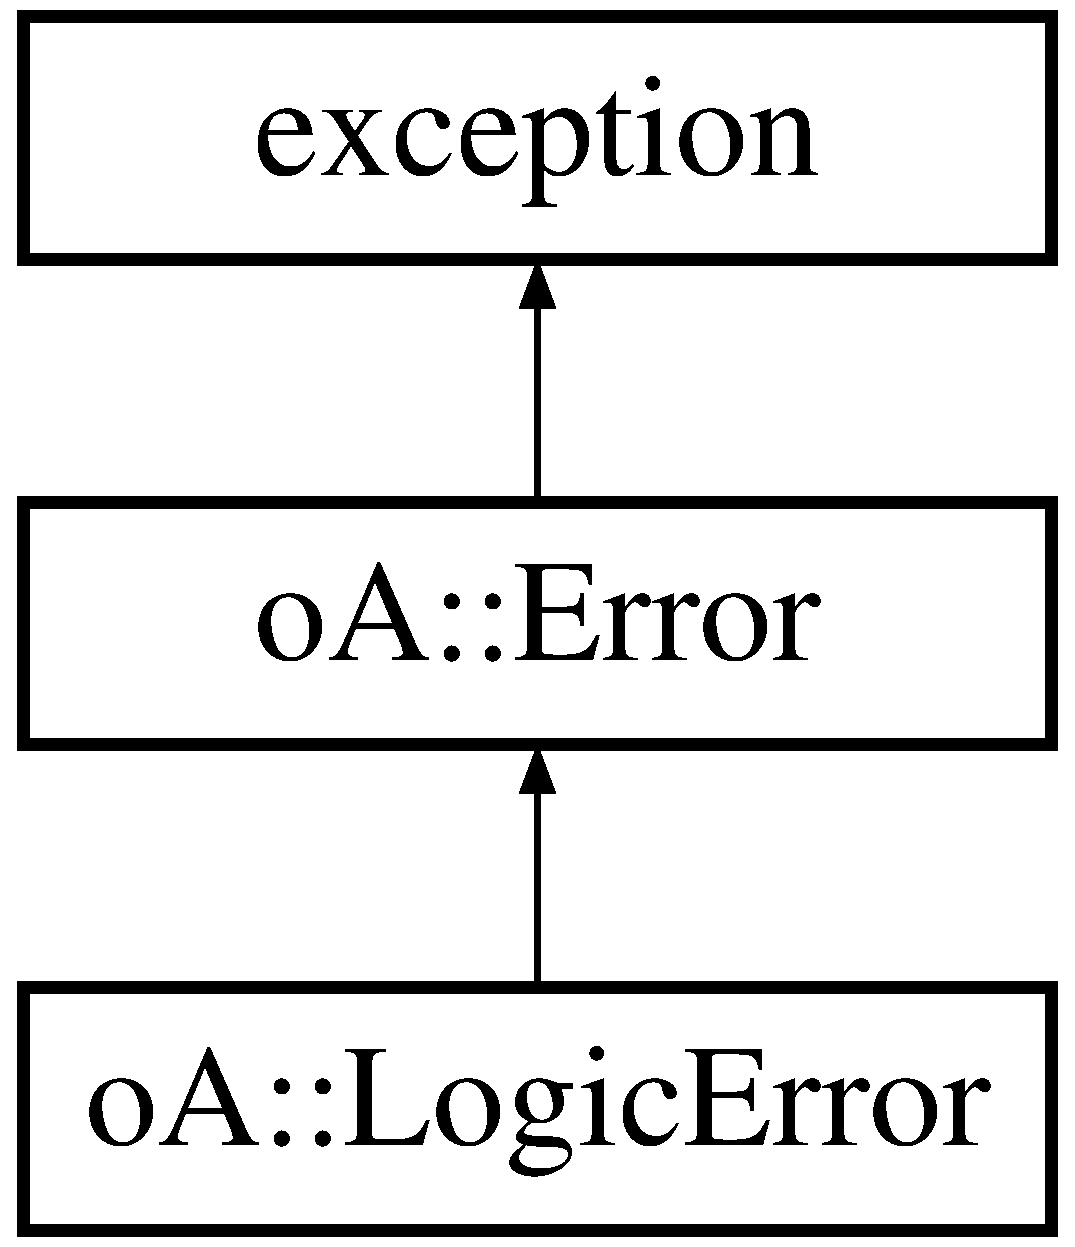
\includegraphics[height=3.000000cm]{classo_a_1_1_logic_error}
\end{center}
\end{figure}
\subsection*{Public Member Functions}
\begin{DoxyCompactItemize}
\item 
\mbox{\hyperlink{classo_a_1_1_logic_error_a16d10704561d2b756722d71d8703089c}{Error}} (const \mbox{\hyperlink{classo_a_1_1_string}{String}} \&msg)
\item 
\mbox{\hyperlink{classo_a_1_1_logic_error_adf66492ca8b03fa14d09e5bba7cdacbd}{Error}} (const \mbox{\hyperlink{classo_a_1_1_string}{String}} \&from, const \mbox{\hyperlink{classo_a_1_1_string}{String}} \&msg)
\end{DoxyCompactItemize}


\subsection{Member Function Documentation}
\mbox{\Hypertarget{classo_a_1_1_logic_error_a16d10704561d2b756722d71d8703089c}\label{classo_a_1_1_logic_error_a16d10704561d2b756722d71d8703089c}} 
\index{o\+A\+::\+Logic\+Error@{o\+A\+::\+Logic\+Error}!Error@{Error}}
\index{Error@{Error}!o\+A\+::\+Logic\+Error@{o\+A\+::\+Logic\+Error}}
\subsubsection{\texorpdfstring{Error()}{Error()}\hspace{0.1cm}{\footnotesize\ttfamily [1/2]}}
{\footnotesize\ttfamily o\+A\+::\+Error\+::\+Error\hspace{0.3cm}{\ttfamily [inline]}}

\mbox{\Hypertarget{classo_a_1_1_logic_error_adf66492ca8b03fa14d09e5bba7cdacbd}\label{classo_a_1_1_logic_error_adf66492ca8b03fa14d09e5bba7cdacbd}} 
\index{o\+A\+::\+Logic\+Error@{o\+A\+::\+Logic\+Error}!Error@{Error}}
\index{Error@{Error}!o\+A\+::\+Logic\+Error@{o\+A\+::\+Logic\+Error}}
\subsubsection{\texorpdfstring{Error()}{Error()}\hspace{0.1cm}{\footnotesize\ttfamily [2/2]}}
{\footnotesize\ttfamily o\+A\+::\+Error\+::\+Error\hspace{0.3cm}{\ttfamily [inline]}}



The documentation for this class was generated from the following file\+:\begin{DoxyCompactItemize}
\item 
Library/open\+App/\+Types/\mbox{\hyperlink{_error_8hpp}{Error.\+hpp}}\end{DoxyCompactItemize}

\hypertarget{structo_a_1_1_overload}{}\section{oA\+:\+:Overload$<$ Args $>$ Struct Template Reference}
\label{structo_a_1_1_overload}\index{o\+A\+::\+Overload$<$ Args $>$@{o\+A\+::\+Overload$<$ Args $>$}}


{\ttfamily \#include $<$Variant.\+hpp$>$}

Inheritance diagram for oA\+:\+:Overload$<$ Args $>$\+:\begin{figure}[H]
\begin{center}
\leavevmode
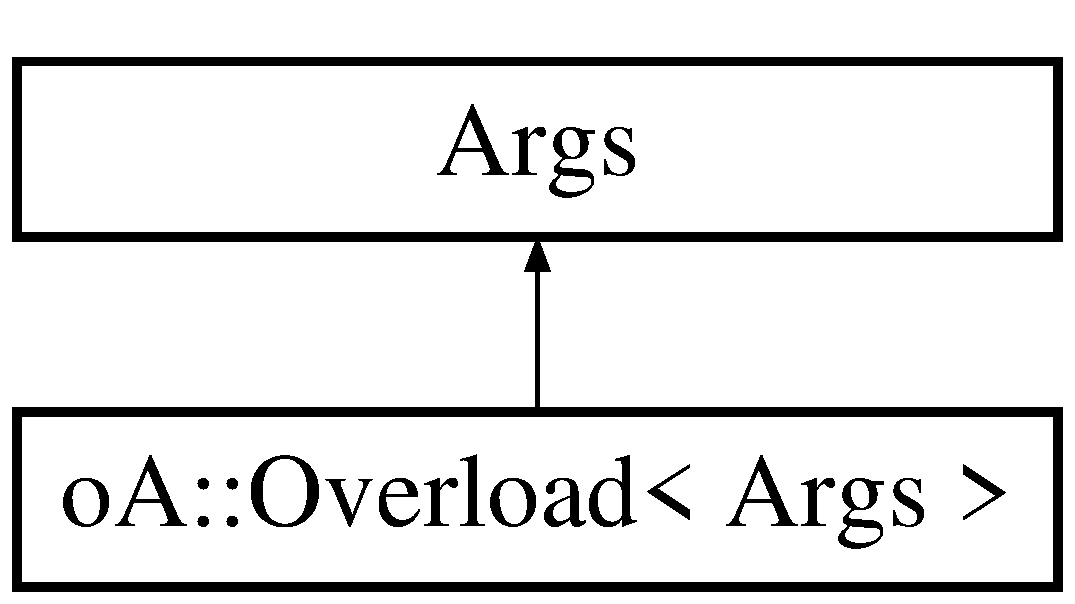
\includegraphics[height=2.000000cm]{structo_a_1_1_overload}
\end{center}
\end{figure}


The documentation for this struct was generated from the following file\+:\begin{DoxyCompactItemize}
\item 
Library/open\+App/\+Types/\mbox{\hyperlink{_variant_8hpp}{Variant.\+hpp}}\end{DoxyCompactItemize}

\hypertarget{classo_a_1_1_quote}{}\section{oA\+:\+:Quote Class Reference}
\label{classo_a_1_1_quote}\index{o\+A\+::\+Quote@{o\+A\+::\+Quote}}


\mbox{\hyperlink{classo_a_1_1_quote}{Quote}} contains a matching symbol and a color.  




{\ttfamily \#include $<$Log\+Utils.\+hpp$>$}



Inheritance diagram for oA\+:\+:Quote\+:
% FIG 0
\subsection*{Public Member Functions}
\begin{DoxyCompactItemize}
\item 
\mbox{\hyperlink{classo_a_1_1_quote_a106d98164983c0d65e8b181275ab763b}{Quote}} (const \mbox{\hyperlink{namespaceo_a_a747e07c1977a29f3e1d38683043ec927}{Console\+Color}} \&\mbox{\hyperlink{classo_a_1_1_quote_a2230c25c43af7317d5ab5785b382f2ce}{color}}, char \mbox{\hyperlink{classo_a_1_1_quote_a3347e15b8ef676b7a5b2017b80e8befc}{match}})
\begin{DoxyCompactList}\small\item\em Construct a new \mbox{\hyperlink{classo_a_1_1_quote}{Quote}} object using a color and a symbol. \end{DoxyCompactList}\item 
char \mbox{\hyperlink{classo_a_1_1_quote_a3347e15b8ef676b7a5b2017b80e8befc}{match}} (void) const noexcept
\begin{DoxyCompactList}\small\item\em Return matching symbol. \end{DoxyCompactList}\item 
const \mbox{\hyperlink{namespaceo_a_a747e07c1977a29f3e1d38683043ec927}{Console\+Color}} \& \mbox{\hyperlink{classo_a_1_1_quote_a2230c25c43af7317d5ab5785b382f2ce}{color}} (void) const noexcept
\begin{DoxyCompactList}\small\item\em Return internal color. \end{DoxyCompactList}\end{DoxyCompactItemize}


\subsection{Detailed Description}
\mbox{\hyperlink{classo_a_1_1_quote}{Quote}} contains a matching symbol and a color. 

This class is used to initialize a \mbox{\hyperlink{classo_a_1_1_log}{Log}} 

\subsection{Constructor \& Destructor Documentation}
\mbox{\Hypertarget{classo_a_1_1_quote_a106d98164983c0d65e8b181275ab763b}\label{classo_a_1_1_quote_a106d98164983c0d65e8b181275ab763b}} 
\index{o\+A\+::\+Quote@{o\+A\+::\+Quote}!Quote@{Quote}}
\index{Quote@{Quote}!o\+A\+::\+Quote@{o\+A\+::\+Quote}}
\subsubsection{\texorpdfstring{Quote()}{Quote()}}
{\footnotesize\ttfamily o\+A\+::\+Quote\+::\+Quote (\begin{DoxyParamCaption}\item[{const \mbox{\hyperlink{namespaceo_a_a747e07c1977a29f3e1d38683043ec927}{Console\+Color}} \&}]{color,  }\item[{char}]{match }\end{DoxyParamCaption})\hspace{0.3cm}{\ttfamily [inline]}}



Construct a new \mbox{\hyperlink{classo_a_1_1_quote}{Quote}} object using a color and a symbol. 


\begin{DoxyParams}{Parameters}
{\em color} & Matching color \\
\hline
{\em match} & Matching character \\
\hline
\end{DoxyParams}


\subsection{Member Function Documentation}
\mbox{\Hypertarget{classo_a_1_1_quote_a2230c25c43af7317d5ab5785b382f2ce}\label{classo_a_1_1_quote_a2230c25c43af7317d5ab5785b382f2ce}} 
\index{o\+A\+::\+Quote@{o\+A\+::\+Quote}!color@{color}}
\index{color@{color}!o\+A\+::\+Quote@{o\+A\+::\+Quote}}
\subsubsection{\texorpdfstring{color()}{color()}}
{\footnotesize\ttfamily const \mbox{\hyperlink{namespaceo_a_a747e07c1977a29f3e1d38683043ec927}{Console\+Color}}\& o\+A\+::\+Quote\+::color (\begin{DoxyParamCaption}\item[{void}]{ }\end{DoxyParamCaption}) const\hspace{0.3cm}{\ttfamily [inline]}, {\ttfamily [noexcept]}}



Return internal color. 

\begin{DoxyReturn}{Returns}
const Console\+Color\& Internal color 
\end{DoxyReturn}
\mbox{\Hypertarget{classo_a_1_1_quote_a3347e15b8ef676b7a5b2017b80e8befc}\label{classo_a_1_1_quote_a3347e15b8ef676b7a5b2017b80e8befc}} 
\index{o\+A\+::\+Quote@{o\+A\+::\+Quote}!match@{match}}
\index{match@{match}!o\+A\+::\+Quote@{o\+A\+::\+Quote}}
\subsubsection{\texorpdfstring{match()}{match()}}
{\footnotesize\ttfamily char o\+A\+::\+Quote\+::match (\begin{DoxyParamCaption}\item[{void}]{ }\end{DoxyParamCaption}) const\hspace{0.3cm}{\ttfamily [inline]}, {\ttfamily [noexcept]}}



Return matching symbol. 

\begin{DoxyReturn}{Returns}
char Matching symbol 
\end{DoxyReturn}


The documentation for this class was generated from the following file\+:\begin{DoxyCompactItemize}
\item 
Library/open\+App/\+Core/\mbox{\hyperlink{_log_utils_8hpp}{Log\+Utils.\+hpp}}\end{DoxyCompactItemize}

\hypertarget{classo_a_1_1_repeat}{}\section{oA\+:\+:Repeat Class Reference}
\label{classo_a_1_1_repeat}\index{o\+A\+::\+Repeat@{o\+A\+::\+Repeat}}


{\ttfamily \#include $<$Log\+Utils.\+hpp$>$}

\subsection*{Public Member Functions}
\begin{DoxyCompactItemize}
\item 
\mbox{\hyperlink{classo_a_1_1_repeat_a2ec587ad895e56ef3c22061a819f4f45}{Repeat}} (void)=default
\item 
\mbox{\hyperlink{classo_a_1_1_repeat_acced7bf3a3daff1434569dc593e2de0e}{Repeat}} (\mbox{\hyperlink{namespaceo_a_abe1d8250226c5cf34f84d7b75fc7922e}{Uint}} times)
\item 
\mbox{\hyperlink{namespaceo_a_abe1d8250226c5cf34f84d7b75fc7922e}{Uint}} \& \mbox{\hyperlink{classo_a_1_1_repeat_aae1cd1f736329d24bebd70a050aec29c}{count}} (void) noexcept
\end{DoxyCompactItemize}


\subsection{Constructor \& Destructor Documentation}
\mbox{\Hypertarget{classo_a_1_1_repeat_a2ec587ad895e56ef3c22061a819f4f45}\label{classo_a_1_1_repeat_a2ec587ad895e56ef3c22061a819f4f45}} 
\index{o\+A\+::\+Repeat@{o\+A\+::\+Repeat}!Repeat@{Repeat}}
\index{Repeat@{Repeat}!o\+A\+::\+Repeat@{o\+A\+::\+Repeat}}
\subsubsection{\texorpdfstring{Repeat()}{Repeat()}\hspace{0.1cm}{\footnotesize\ttfamily [1/2]}}
{\footnotesize\ttfamily o\+A\+::\+Repeat\+::\+Repeat (\begin{DoxyParamCaption}\item[{void}]{ }\end{DoxyParamCaption})\hspace{0.3cm}{\ttfamily [default]}}

\mbox{\Hypertarget{classo_a_1_1_repeat_acced7bf3a3daff1434569dc593e2de0e}\label{classo_a_1_1_repeat_acced7bf3a3daff1434569dc593e2de0e}} 
\index{o\+A\+::\+Repeat@{o\+A\+::\+Repeat}!Repeat@{Repeat}}
\index{Repeat@{Repeat}!o\+A\+::\+Repeat@{o\+A\+::\+Repeat}}
\subsubsection{\texorpdfstring{Repeat()}{Repeat()}\hspace{0.1cm}{\footnotesize\ttfamily [2/2]}}
{\footnotesize\ttfamily o\+A\+::\+Repeat\+::\+Repeat (\begin{DoxyParamCaption}\item[{\mbox{\hyperlink{namespaceo_a_abe1d8250226c5cf34f84d7b75fc7922e}{Uint}}}]{times }\end{DoxyParamCaption})\hspace{0.3cm}{\ttfamily [inline]}}



\subsection{Member Function Documentation}
\mbox{\Hypertarget{classo_a_1_1_repeat_aae1cd1f736329d24bebd70a050aec29c}\label{classo_a_1_1_repeat_aae1cd1f736329d24bebd70a050aec29c}} 
\index{o\+A\+::\+Repeat@{o\+A\+::\+Repeat}!count@{count}}
\index{count@{count}!o\+A\+::\+Repeat@{o\+A\+::\+Repeat}}
\subsubsection{\texorpdfstring{count()}{count()}}
{\footnotesize\ttfamily \mbox{\hyperlink{namespaceo_a_abe1d8250226c5cf34f84d7b75fc7922e}{Uint}}\& o\+A\+::\+Repeat\+::count (\begin{DoxyParamCaption}\item[{void}]{ }\end{DoxyParamCaption})\hspace{0.3cm}{\ttfamily [inline]}, {\ttfamily [noexcept]}}



The documentation for this class was generated from the following file\+:\begin{DoxyCompactItemize}
\item 
Library/open\+App/\+Core/\mbox{\hyperlink{_log_utils_8hpp}{Log\+Utils.\+hpp}}\end{DoxyCompactItemize}

\hypertarget{classo_a_1_1_string}{}\section{oA\+:\+:String Class Reference}
\label{classo_a_1_1_string}\index{o\+A\+::\+String@{o\+A\+::\+String}}


An extended std\+::string with \mbox{\hyperlink{classo_a_1_1_container_helper}{Container\+Helper}} and various helper functions.  




{\ttfamily \#include $<$String.\+hpp$>$}



Inheritance diagram for oA\+:\+:String\+:
% FIG 0


Collaboration diagram for oA\+:\+:String\+:
% FIG 1
\subsection*{Public Member Functions}
\begin{DoxyCompactItemize}
\item 
\mbox{\hyperlink{classo_a_1_1_string_a10ce41917f151b304f0b465c1ff1ec6e}{String}} (void)
\begin{DoxyCompactList}\small\item\em Construct a new \mbox{\hyperlink{classo_a_1_1_string}{String}} object. \end{DoxyCompactList}\item 
\mbox{\hyperlink{classo_a_1_1_string_adeb13912c55cdc0406b5960d75d74fb2}{String}} (const \mbox{\hyperlink{classo_a_1_1_string}{String}} \&other)
\begin{DoxyCompactList}\small\item\em Construct a new \mbox{\hyperlink{classo_a_1_1_string}{String}} object by copy. \end{DoxyCompactList}\item 
\mbox{\hyperlink{classo_a_1_1_string_ae728fbb314314b37c103d3b22ca4c3a9}{String}} (\mbox{\hyperlink{classo_a_1_1_string}{String}} \&\&other)
\begin{DoxyCompactList}\small\item\em Construct a new \mbox{\hyperlink{classo_a_1_1_string}{String}} object by move. \end{DoxyCompactList}\item 
\mbox{\hyperlink{classo_a_1_1_string_a7406ec03e50352320d8809a78e12a9fa}{String}} (const std\+::string \&other)
\begin{DoxyCompactList}\small\item\em Construct a new \mbox{\hyperlink{classo_a_1_1_string}{String}} object with a std\+::string by copy. \end{DoxyCompactList}\item 
\mbox{\hyperlink{classo_a_1_1_string_a0b5007bec6fe6f6c8917ecc4febbbd1c}{String}} (std\+::string \&\&other)
\begin{DoxyCompactList}\small\item\em Construct a new \mbox{\hyperlink{classo_a_1_1_string}{String}} object with a std\+::string by move. \end{DoxyCompactList}\item 
\mbox{\hyperlink{classo_a_1_1_string_a5289dc4246f8adf29ade43156ad4a703}{String}} (char c)
\begin{DoxyCompactList}\small\item\em Construct a new \mbox{\hyperlink{classo_a_1_1_string}{String}} object with a char. \end{DoxyCompactList}\item 
\mbox{\hyperlink{classo_a_1_1_string_adee64db6ad1f06dc35c6e960811d3734}{String}} (const char $\ast$const raw)
\begin{DoxyCompactList}\small\item\em Construct a new \mbox{\hyperlink{classo_a_1_1_string}{String}} object with a raw C char pointer. \end{DoxyCompactList}\item 
\mbox{\hyperlink{classo_a_1_1_string_abc7b54346e6c161fb0365336cda41957}{operator bool}} (void) const noexcept
\begin{DoxyCompactList}\small\item\em Return internal string state (true if not empty) \end{DoxyCompactList}\item 
\mbox{\hyperlink{classo_a_1_1_string}{String}} \& \mbox{\hyperlink{classo_a_1_1_string_ac979bb3953e566011543bd0ebe78e822}{operator=}} (const \mbox{\hyperlink{classo_a_1_1_string}{String}} \&other) noexcept
\begin{DoxyCompactList}\small\item\em Copy assignement operator. \end{DoxyCompactList}\item 
\mbox{\hyperlink{classo_a_1_1_string}{String}} \& \mbox{\hyperlink{classo_a_1_1_string_ab45f150390030ee04c119399a4c9fbb7}{operator=}} (\mbox{\hyperlink{classo_a_1_1_string}{String}} \&\&other) noexcept
\begin{DoxyCompactList}\small\item\em Move assignement operator. \end{DoxyCompactList}\item 
\mbox{\hyperlink{classo_a_1_1_string}{String}} \& \mbox{\hyperlink{classo_a_1_1_string_a748a9d3de7d14593f24d5e82fc306413}{operator+=}} (const \mbox{\hyperlink{classo_a_1_1_string}{String}} \&other) noexcept
\begin{DoxyCompactList}\small\item\em Append operator by copy. \end{DoxyCompactList}\item 
\mbox{\hyperlink{classo_a_1_1_string}{String}} \& \mbox{\hyperlink{classo_a_1_1_string_a99849336461c58e51681c68acd1fcafc}{operator+=}} (\mbox{\hyperlink{classo_a_1_1_string}{String}} \&\&other) noexcept
\begin{DoxyCompactList}\small\item\em Append operator by move. \end{DoxyCompactList}\item 
bool \mbox{\hyperlink{classo_a_1_1_string_a838537de7617a227e77662090f25d5a9}{to\+Bool}} (void) const
\begin{DoxyCompactList}\small\item\em Boolean cast. \end{DoxyCompactList}\item 
\mbox{\hyperlink{namespaceo_a_aa575525a7b0116822c73d43fa671a58c}{Int}} \mbox{\hyperlink{classo_a_1_1_string_a8aab531770e6d4abe2a3e85d55f69ead}{to\+Int}} (void) const
\begin{DoxyCompactList}\small\item\em Int cast. \end{DoxyCompactList}\item 
\mbox{\hyperlink{namespaceo_a_abe1d8250226c5cf34f84d7b75fc7922e}{Uint}} \mbox{\hyperlink{classo_a_1_1_string_a959f6a81bf2fa3e6fa001642608e2af2}{to\+Uint}} (void) const
\begin{DoxyCompactList}\small\item\em Uint cast. \end{DoxyCompactList}\item 
\mbox{\hyperlink{namespaceo_a_a513e9cb16924b482268ab3fcdf1f2499}{Float}} \mbox{\hyperlink{classo_a_1_1_string_a109668ec1795a27a5c44b33ec53e56a3}{to\+Float}} (void) const
\begin{DoxyCompactList}\small\item\em Float cast. \end{DoxyCompactList}\item 
\mbox{\hyperlink{namespaceo_a_a2bcc976232176d2dcf8b9df1fa33c038}{Double}} \mbox{\hyperlink{classo_a_1_1_string_a609bc93f4fdb26cc79d26747741af787}{to\+Double}} (void) const
\begin{DoxyCompactList}\small\item\em Double cast. \end{DoxyCompactList}\item 
bool \mbox{\hyperlink{classo_a_1_1_string_af57b0b992d2ce2995f3f843d7dd36e96}{is\+Boolean}} (void) const noexcept
\begin{DoxyCompactList}\small\item\em Boolean check. \end{DoxyCompactList}\item 
bool \mbox{\hyperlink{classo_a_1_1_string_ac88615009b2cdba26d1bf42187a66eb7}{is\+Signed}} (void) const noexcept
\begin{DoxyCompactList}\small\item\em Signed check. \end{DoxyCompactList}\item 
bool \mbox{\hyperlink{classo_a_1_1_string_aeb851821fb8dd5ca72d50413f72bb1a4}{is\+Unsigned}} (void) const noexcept
\begin{DoxyCompactList}\small\item\em Unsigned check. \end{DoxyCompactList}\item 
bool \mbox{\hyperlink{classo_a_1_1_string_a30effa3311ecb3f5f29e8d670709f436}{is\+Decimal}} (void) const noexcept
\begin{DoxyCompactList}\small\item\em Decimal check. \end{DoxyCompactList}\item 
void \mbox{\hyperlink{classo_a_1_1_string_a54760c3b5fee78fbcc28a6d81dbfe6b3}{replace}} (const \mbox{\hyperlink{classo_a_1_1_string}{String}} \&from, const \mbox{\hyperlink{classo_a_1_1_string}{String}} \&to)
\begin{DoxyCompactList}\small\item\em Replace each occurence of a given sequence with another. \end{DoxyCompactList}\item 
void \mbox{\hyperlink{classo_a_1_1_string_a9f974d8b83a0ae4232a33d249291f3c4}{replace\+With}} (const \mbox{\hyperlink{classo_a_1_1_string}{String}} \&from, const \mbox{\hyperlink{namespaceo_a_a85bea86b9d05d2b86c77d8ee5b7bbde5}{Function}}$<$ \mbox{\hyperlink{classo_a_1_1_string}{String}}(void)$>$ \&to)
\begin{DoxyCompactList}\small\item\em Replace each occurence of a given sequence with the result of a lambda. \end{DoxyCompactList}\end{DoxyCompactItemize}


\subsection{Detailed Description}
An extended std\+::string with \mbox{\hyperlink{classo_a_1_1_container_helper}{Container\+Helper}} and various helper functions. 

\subsection{Constructor \& Destructor Documentation}
\mbox{\Hypertarget{classo_a_1_1_string_a10ce41917f151b304f0b465c1ff1ec6e}\label{classo_a_1_1_string_a10ce41917f151b304f0b465c1ff1ec6e}} 
\index{o\+A\+::\+String@{o\+A\+::\+String}!String@{String}}
\index{String@{String}!o\+A\+::\+String@{o\+A\+::\+String}}
\subsubsection{\texorpdfstring{String()}{String()}\hspace{0.1cm}{\footnotesize\ttfamily [1/7]}}
{\footnotesize\ttfamily o\+A\+::\+String\+::\+String (\begin{DoxyParamCaption}\item[{void}]{ }\end{DoxyParamCaption})\hspace{0.3cm}{\ttfamily [inline]}}



Construct a new \mbox{\hyperlink{classo_a_1_1_string}{String}} object. 

\mbox{\Hypertarget{classo_a_1_1_string_adeb13912c55cdc0406b5960d75d74fb2}\label{classo_a_1_1_string_adeb13912c55cdc0406b5960d75d74fb2}} 
\index{o\+A\+::\+String@{o\+A\+::\+String}!String@{String}}
\index{String@{String}!o\+A\+::\+String@{o\+A\+::\+String}}
\subsubsection{\texorpdfstring{String()}{String()}\hspace{0.1cm}{\footnotesize\ttfamily [2/7]}}
{\footnotesize\ttfamily o\+A\+::\+String\+::\+String (\begin{DoxyParamCaption}\item[{const \mbox{\hyperlink{classo_a_1_1_string}{String}} \&}]{other }\end{DoxyParamCaption})\hspace{0.3cm}{\ttfamily [inline]}}



Construct a new \mbox{\hyperlink{classo_a_1_1_string}{String}} object by copy. 


\begin{DoxyParams}{Parameters}
{\em other} & Variable to copy \\
\hline
\end{DoxyParams}
\mbox{\Hypertarget{classo_a_1_1_string_ae728fbb314314b37c103d3b22ca4c3a9}\label{classo_a_1_1_string_ae728fbb314314b37c103d3b22ca4c3a9}} 
\index{o\+A\+::\+String@{o\+A\+::\+String}!String@{String}}
\index{String@{String}!o\+A\+::\+String@{o\+A\+::\+String}}
\subsubsection{\texorpdfstring{String()}{String()}\hspace{0.1cm}{\footnotesize\ttfamily [3/7]}}
{\footnotesize\ttfamily o\+A\+::\+String\+::\+String (\begin{DoxyParamCaption}\item[{\mbox{\hyperlink{classo_a_1_1_string}{String}} \&\&}]{other }\end{DoxyParamCaption})\hspace{0.3cm}{\ttfamily [inline]}}



Construct a new \mbox{\hyperlink{classo_a_1_1_string}{String}} object by move. 


\begin{DoxyParams}{Parameters}
{\em other} & Variable to move \\
\hline
\end{DoxyParams}
\mbox{\Hypertarget{classo_a_1_1_string_a7406ec03e50352320d8809a78e12a9fa}\label{classo_a_1_1_string_a7406ec03e50352320d8809a78e12a9fa}} 
\index{o\+A\+::\+String@{o\+A\+::\+String}!String@{String}}
\index{String@{String}!o\+A\+::\+String@{o\+A\+::\+String}}
\subsubsection{\texorpdfstring{String()}{String()}\hspace{0.1cm}{\footnotesize\ttfamily [4/7]}}
{\footnotesize\ttfamily o\+A\+::\+String\+::\+String (\begin{DoxyParamCaption}\item[{const std\+::string \&}]{other }\end{DoxyParamCaption})\hspace{0.3cm}{\ttfamily [inline]}}



Construct a new \mbox{\hyperlink{classo_a_1_1_string}{String}} object with a std\+::string by copy. 


\begin{DoxyParams}{Parameters}
{\em other} & Variable to copy \\
\hline
\end{DoxyParams}
\mbox{\Hypertarget{classo_a_1_1_string_a0b5007bec6fe6f6c8917ecc4febbbd1c}\label{classo_a_1_1_string_a0b5007bec6fe6f6c8917ecc4febbbd1c}} 
\index{o\+A\+::\+String@{o\+A\+::\+String}!String@{String}}
\index{String@{String}!o\+A\+::\+String@{o\+A\+::\+String}}
\subsubsection{\texorpdfstring{String()}{String()}\hspace{0.1cm}{\footnotesize\ttfamily [5/7]}}
{\footnotesize\ttfamily o\+A\+::\+String\+::\+String (\begin{DoxyParamCaption}\item[{std\+::string \&\&}]{other }\end{DoxyParamCaption})\hspace{0.3cm}{\ttfamily [inline]}}



Construct a new \mbox{\hyperlink{classo_a_1_1_string}{String}} object with a std\+::string by move. 


\begin{DoxyParams}{Parameters}
{\em other} & Variable to move \\
\hline
\end{DoxyParams}
\mbox{\Hypertarget{classo_a_1_1_string_a5289dc4246f8adf29ade43156ad4a703}\label{classo_a_1_1_string_a5289dc4246f8adf29ade43156ad4a703}} 
\index{o\+A\+::\+String@{o\+A\+::\+String}!String@{String}}
\index{String@{String}!o\+A\+::\+String@{o\+A\+::\+String}}
\subsubsection{\texorpdfstring{String()}{String()}\hspace{0.1cm}{\footnotesize\ttfamily [6/7]}}
{\footnotesize\ttfamily o\+A\+::\+String\+::\+String (\begin{DoxyParamCaption}\item[{char}]{c }\end{DoxyParamCaption})\hspace{0.3cm}{\ttfamily [inline]}}



Construct a new \mbox{\hyperlink{classo_a_1_1_string}{String}} object with a char. 


\begin{DoxyParams}{Parameters}
{\em c} & Char to insert \\
\hline
\end{DoxyParams}
\mbox{\Hypertarget{classo_a_1_1_string_adee64db6ad1f06dc35c6e960811d3734}\label{classo_a_1_1_string_adee64db6ad1f06dc35c6e960811d3734}} 
\index{o\+A\+::\+String@{o\+A\+::\+String}!String@{String}}
\index{String@{String}!o\+A\+::\+String@{o\+A\+::\+String}}
\subsubsection{\texorpdfstring{String()}{String()}\hspace{0.1cm}{\footnotesize\ttfamily [7/7]}}
{\footnotesize\ttfamily o\+A\+::\+String\+::\+String (\begin{DoxyParamCaption}\item[{const char $\ast$const}]{raw }\end{DoxyParamCaption})\hspace{0.3cm}{\ttfamily [inline]}}



Construct a new \mbox{\hyperlink{classo_a_1_1_string}{String}} object with a raw C char pointer. 


\begin{DoxyParams}{Parameters}
{\em raw} & C string to copy \\
\hline
\end{DoxyParams}


\subsection{Member Function Documentation}
\mbox{\Hypertarget{classo_a_1_1_string_af57b0b992d2ce2995f3f843d7dd36e96}\label{classo_a_1_1_string_af57b0b992d2ce2995f3f843d7dd36e96}} 
\index{o\+A\+::\+String@{o\+A\+::\+String}!is\+Boolean@{is\+Boolean}}
\index{is\+Boolean@{is\+Boolean}!o\+A\+::\+String@{o\+A\+::\+String}}
\subsubsection{\texorpdfstring{is\+Boolean()}{isBoolean()}}
{\footnotesize\ttfamily bool o\+A\+::\+String\+::is\+Boolean (\begin{DoxyParamCaption}\item[{void}]{ }\end{DoxyParamCaption}) const\hspace{0.3cm}{\ttfamily [noexcept]}}



Boolean check. 

\begin{DoxyReturn}{Returns}
bool Return if the Boolean cast is possible 
\end{DoxyReturn}
\mbox{\Hypertarget{classo_a_1_1_string_a30effa3311ecb3f5f29e8d670709f436}\label{classo_a_1_1_string_a30effa3311ecb3f5f29e8d670709f436}} 
\index{o\+A\+::\+String@{o\+A\+::\+String}!is\+Decimal@{is\+Decimal}}
\index{is\+Decimal@{is\+Decimal}!o\+A\+::\+String@{o\+A\+::\+String}}
\subsubsection{\texorpdfstring{is\+Decimal()}{isDecimal()}}
{\footnotesize\ttfamily bool o\+A\+::\+String\+::is\+Decimal (\begin{DoxyParamCaption}\item[{void}]{ }\end{DoxyParamCaption}) const\hspace{0.3cm}{\ttfamily [noexcept]}}



Decimal check. 

\begin{DoxyReturn}{Returns}
bool Return if the Decimal cast is possible 
\end{DoxyReturn}
\mbox{\Hypertarget{classo_a_1_1_string_ac88615009b2cdba26d1bf42187a66eb7}\label{classo_a_1_1_string_ac88615009b2cdba26d1bf42187a66eb7}} 
\index{o\+A\+::\+String@{o\+A\+::\+String}!is\+Signed@{is\+Signed}}
\index{is\+Signed@{is\+Signed}!o\+A\+::\+String@{o\+A\+::\+String}}
\subsubsection{\texorpdfstring{is\+Signed()}{isSigned()}}
{\footnotesize\ttfamily bool o\+A\+::\+String\+::is\+Signed (\begin{DoxyParamCaption}\item[{void}]{ }\end{DoxyParamCaption}) const\hspace{0.3cm}{\ttfamily [noexcept]}}



Signed check. 

\begin{DoxyReturn}{Returns}
bool Return if the Signed cast is possible 
\end{DoxyReturn}
\mbox{\Hypertarget{classo_a_1_1_string_aeb851821fb8dd5ca72d50413f72bb1a4}\label{classo_a_1_1_string_aeb851821fb8dd5ca72d50413f72bb1a4}} 
\index{o\+A\+::\+String@{o\+A\+::\+String}!is\+Unsigned@{is\+Unsigned}}
\index{is\+Unsigned@{is\+Unsigned}!o\+A\+::\+String@{o\+A\+::\+String}}
\subsubsection{\texorpdfstring{is\+Unsigned()}{isUnsigned()}}
{\footnotesize\ttfamily bool o\+A\+::\+String\+::is\+Unsigned (\begin{DoxyParamCaption}\item[{void}]{ }\end{DoxyParamCaption}) const\hspace{0.3cm}{\ttfamily [noexcept]}}



Unsigned check. 

\begin{DoxyReturn}{Returns}
bool Return if the Unsigned cast is possible 
\end{DoxyReturn}
\mbox{\Hypertarget{classo_a_1_1_string_abc7b54346e6c161fb0365336cda41957}\label{classo_a_1_1_string_abc7b54346e6c161fb0365336cda41957}} 
\index{o\+A\+::\+String@{o\+A\+::\+String}!operator bool@{operator bool}}
\index{operator bool@{operator bool}!o\+A\+::\+String@{o\+A\+::\+String}}
\subsubsection{\texorpdfstring{operator bool()}{operator bool()}}
{\footnotesize\ttfamily o\+A\+::\+String\+::operator bool (\begin{DoxyParamCaption}\item[{void}]{ }\end{DoxyParamCaption}) const\hspace{0.3cm}{\ttfamily [inline]}, {\ttfamily [noexcept]}}



Return internal string state (true if not empty) 

\mbox{\Hypertarget{classo_a_1_1_string_a748a9d3de7d14593f24d5e82fc306413}\label{classo_a_1_1_string_a748a9d3de7d14593f24d5e82fc306413}} 
\index{o\+A\+::\+String@{o\+A\+::\+String}!operator+=@{operator+=}}
\index{operator+=@{operator+=}!o\+A\+::\+String@{o\+A\+::\+String}}
\subsubsection{\texorpdfstring{operator+=()}{operator+=()}\hspace{0.1cm}{\footnotesize\ttfamily [1/2]}}
{\footnotesize\ttfamily \mbox{\hyperlink{classo_a_1_1_string}{o\+A\+::\+String}} \& o\+A\+::\+String\+::operator+= (\begin{DoxyParamCaption}\item[{const \mbox{\hyperlink{classo_a_1_1_string}{String}} \&}]{other }\end{DoxyParamCaption})\hspace{0.3cm}{\ttfamily [noexcept]}}



Append operator by copy. 


\begin{DoxyParams}{Parameters}
{\em other} & Value to append \\
\hline
\end{DoxyParams}
\begin{DoxyReturn}{Returns}
\mbox{\hyperlink{classo_a_1_1_string}{String}}\& Allow chain operators 
\end{DoxyReturn}
\mbox{\Hypertarget{classo_a_1_1_string_a99849336461c58e51681c68acd1fcafc}\label{classo_a_1_1_string_a99849336461c58e51681c68acd1fcafc}} 
\index{o\+A\+::\+String@{o\+A\+::\+String}!operator+=@{operator+=}}
\index{operator+=@{operator+=}!o\+A\+::\+String@{o\+A\+::\+String}}
\subsubsection{\texorpdfstring{operator+=()}{operator+=()}\hspace{0.1cm}{\footnotesize\ttfamily [2/2]}}
{\footnotesize\ttfamily \mbox{\hyperlink{classo_a_1_1_string}{o\+A\+::\+String}} \& o\+A\+::\+String\+::operator+= (\begin{DoxyParamCaption}\item[{\mbox{\hyperlink{classo_a_1_1_string}{String}} \&\&}]{other }\end{DoxyParamCaption})\hspace{0.3cm}{\ttfamily [noexcept]}}



Append operator by move. 


\begin{DoxyParams}{Parameters}
{\em other} & Value to append \\
\hline
\end{DoxyParams}
\begin{DoxyReturn}{Returns}
\mbox{\hyperlink{classo_a_1_1_string}{String}}\& Allow chain operators 
\end{DoxyReturn}
\mbox{\Hypertarget{classo_a_1_1_string_ac979bb3953e566011543bd0ebe78e822}\label{classo_a_1_1_string_ac979bb3953e566011543bd0ebe78e822}} 
\index{o\+A\+::\+String@{o\+A\+::\+String}!operator=@{operator=}}
\index{operator=@{operator=}!o\+A\+::\+String@{o\+A\+::\+String}}
\subsubsection{\texorpdfstring{operator=()}{operator=()}\hspace{0.1cm}{\footnotesize\ttfamily [1/2]}}
{\footnotesize\ttfamily \mbox{\hyperlink{classo_a_1_1_string}{o\+A\+::\+String}} \& o\+A\+::\+String\+::operator= (\begin{DoxyParamCaption}\item[{const \mbox{\hyperlink{classo_a_1_1_string}{String}} \&}]{other }\end{DoxyParamCaption})\hspace{0.3cm}{\ttfamily [noexcept]}}



Copy assignement operator. 


\begin{DoxyParams}{Parameters}
{\em other} & Value to copy \\
\hline
\end{DoxyParams}
\begin{DoxyReturn}{Returns}
\mbox{\hyperlink{classo_a_1_1_string}{String}}\& Allow chain operators 
\end{DoxyReturn}
\mbox{\Hypertarget{classo_a_1_1_string_ab45f150390030ee04c119399a4c9fbb7}\label{classo_a_1_1_string_ab45f150390030ee04c119399a4c9fbb7}} 
\index{o\+A\+::\+String@{o\+A\+::\+String}!operator=@{operator=}}
\index{operator=@{operator=}!o\+A\+::\+String@{o\+A\+::\+String}}
\subsubsection{\texorpdfstring{operator=()}{operator=()}\hspace{0.1cm}{\footnotesize\ttfamily [2/2]}}
{\footnotesize\ttfamily \mbox{\hyperlink{classo_a_1_1_string}{o\+A\+::\+String}} \& o\+A\+::\+String\+::operator= (\begin{DoxyParamCaption}\item[{\mbox{\hyperlink{classo_a_1_1_string}{String}} \&\&}]{other }\end{DoxyParamCaption})\hspace{0.3cm}{\ttfamily [noexcept]}}



Move assignement operator. 


\begin{DoxyParams}{Parameters}
{\em other} & Value to move \\
\hline
\end{DoxyParams}
\begin{DoxyReturn}{Returns}
\mbox{\hyperlink{classo_a_1_1_string}{String}}\& Allow chain operators 
\end{DoxyReturn}
\mbox{\Hypertarget{classo_a_1_1_string_a54760c3b5fee78fbcc28a6d81dbfe6b3}\label{classo_a_1_1_string_a54760c3b5fee78fbcc28a6d81dbfe6b3}} 
\index{o\+A\+::\+String@{o\+A\+::\+String}!replace@{replace}}
\index{replace@{replace}!o\+A\+::\+String@{o\+A\+::\+String}}
\subsubsection{\texorpdfstring{replace()}{replace()}}
{\footnotesize\ttfamily void o\+A\+::\+String\+::replace (\begin{DoxyParamCaption}\item[{const \mbox{\hyperlink{classo_a_1_1_string}{String}} \&}]{from,  }\item[{const \mbox{\hyperlink{classo_a_1_1_string}{String}} \&}]{to }\end{DoxyParamCaption})}



Replace each occurence of a given sequence with another. 


\begin{DoxyParams}{Parameters}
{\em from} & To replace sequence \\
\hline
{\em to} & To insert sequence \\
\hline
\end{DoxyParams}
\mbox{\Hypertarget{classo_a_1_1_string_a9f974d8b83a0ae4232a33d249291f3c4}\label{classo_a_1_1_string_a9f974d8b83a0ae4232a33d249291f3c4}} 
\index{o\+A\+::\+String@{o\+A\+::\+String}!replace\+With@{replace\+With}}
\index{replace\+With@{replace\+With}!o\+A\+::\+String@{o\+A\+::\+String}}
\subsubsection{\texorpdfstring{replace\+With()}{replaceWith()}}
{\footnotesize\ttfamily void o\+A\+::\+String\+::replace\+With (\begin{DoxyParamCaption}\item[{const \mbox{\hyperlink{classo_a_1_1_string}{String}} \&}]{from,  }\item[{const \mbox{\hyperlink{namespaceo_a_a85bea86b9d05d2b86c77d8ee5b7bbde5}{Function}}$<$ \mbox{\hyperlink{classo_a_1_1_string}{String}}(void)$>$ \&}]{to }\end{DoxyParamCaption})}



Replace each occurence of a given sequence with the result of a lambda. 


\begin{DoxyParams}{Parameters}
{\em from} & To replace sequence \\
\hline
{\em to} & Lambda function returing a \mbox{\hyperlink{classo_a_1_1_string}{String}} \\
\hline
\end{DoxyParams}
\mbox{\Hypertarget{classo_a_1_1_string_a838537de7617a227e77662090f25d5a9}\label{classo_a_1_1_string_a838537de7617a227e77662090f25d5a9}} 
\index{o\+A\+::\+String@{o\+A\+::\+String}!to\+Bool@{to\+Bool}}
\index{to\+Bool@{to\+Bool}!o\+A\+::\+String@{o\+A\+::\+String}}
\subsubsection{\texorpdfstring{to\+Bool()}{toBool()}}
{\footnotesize\ttfamily bool o\+A\+::\+String\+::to\+Bool (\begin{DoxyParamCaption}\item[{void}]{ }\end{DoxyParamCaption}) const}



Boolean cast. 

\begin{DoxyReturn}{Returns}
bool Cast result 
\end{DoxyReturn}
\mbox{\Hypertarget{classo_a_1_1_string_a609bc93f4fdb26cc79d26747741af787}\label{classo_a_1_1_string_a609bc93f4fdb26cc79d26747741af787}} 
\index{o\+A\+::\+String@{o\+A\+::\+String}!to\+Double@{to\+Double}}
\index{to\+Double@{to\+Double}!o\+A\+::\+String@{o\+A\+::\+String}}
\subsubsection{\texorpdfstring{to\+Double()}{toDouble()}}
{\footnotesize\ttfamily \mbox{\hyperlink{namespaceo_a_a2bcc976232176d2dcf8b9df1fa33c038}{o\+A\+::\+Double}} o\+A\+::\+String\+::to\+Double (\begin{DoxyParamCaption}\item[{void}]{ }\end{DoxyParamCaption}) const}



Double cast. 

\begin{DoxyReturn}{Returns}
Double Cast result 
\end{DoxyReturn}
\mbox{\Hypertarget{classo_a_1_1_string_a109668ec1795a27a5c44b33ec53e56a3}\label{classo_a_1_1_string_a109668ec1795a27a5c44b33ec53e56a3}} 
\index{o\+A\+::\+String@{o\+A\+::\+String}!to\+Float@{to\+Float}}
\index{to\+Float@{to\+Float}!o\+A\+::\+String@{o\+A\+::\+String}}
\subsubsection{\texorpdfstring{to\+Float()}{toFloat()}}
{\footnotesize\ttfamily \mbox{\hyperlink{namespaceo_a_a513e9cb16924b482268ab3fcdf1f2499}{o\+A\+::\+Float}} o\+A\+::\+String\+::to\+Float (\begin{DoxyParamCaption}\item[{void}]{ }\end{DoxyParamCaption}) const}



Float cast. 

\begin{DoxyReturn}{Returns}
Float Cast result 
\end{DoxyReturn}
\mbox{\Hypertarget{classo_a_1_1_string_a8aab531770e6d4abe2a3e85d55f69ead}\label{classo_a_1_1_string_a8aab531770e6d4abe2a3e85d55f69ead}} 
\index{o\+A\+::\+String@{o\+A\+::\+String}!to\+Int@{to\+Int}}
\index{to\+Int@{to\+Int}!o\+A\+::\+String@{o\+A\+::\+String}}
\subsubsection{\texorpdfstring{to\+Int()}{toInt()}}
{\footnotesize\ttfamily \mbox{\hyperlink{namespaceo_a_aa575525a7b0116822c73d43fa671a58c}{o\+A\+::\+Int}} o\+A\+::\+String\+::to\+Int (\begin{DoxyParamCaption}\item[{void}]{ }\end{DoxyParamCaption}) const}



Int cast. 

\begin{DoxyReturn}{Returns}
Int Cast result 
\end{DoxyReturn}
\mbox{\Hypertarget{classo_a_1_1_string_a959f6a81bf2fa3e6fa001642608e2af2}\label{classo_a_1_1_string_a959f6a81bf2fa3e6fa001642608e2af2}} 
\index{o\+A\+::\+String@{o\+A\+::\+String}!to\+Uint@{to\+Uint}}
\index{to\+Uint@{to\+Uint}!o\+A\+::\+String@{o\+A\+::\+String}}
\subsubsection{\texorpdfstring{to\+Uint()}{toUint()}}
{\footnotesize\ttfamily \mbox{\hyperlink{namespaceo_a_abe1d8250226c5cf34f84d7b75fc7922e}{o\+A\+::\+Uint}} o\+A\+::\+String\+::to\+Uint (\begin{DoxyParamCaption}\item[{void}]{ }\end{DoxyParamCaption}) const}



Uint cast. 

\begin{DoxyReturn}{Returns}
Uint Cast result 
\end{DoxyReturn}


The documentation for this class was generated from the following files\+:\begin{DoxyCompactItemize}
\item 
Library/open\+App/\+Types/\mbox{\hyperlink{_string_8hpp}{String.\+hpp}}\item 
Library/open\+App/\+Types/\mbox{\hyperlink{_string_8cpp}{String.\+cpp}}\end{DoxyCompactItemize}

\hypertarget{structo_a_1_1_v2}{}\section{oA\+:\+:V2$<$ T $>$ Struct Template Reference}
\label{structo_a_1_1_v2}\index{o\+A\+::\+V2$<$ T $>$@{o\+A\+::\+V2$<$ T $>$}}


Vector of 2, similar to a 2D point of type T.  




{\ttfamily \#include $<$V2.\+hpp$>$}

\subsection*{Public Member Functions}
\begin{DoxyCompactItemize}
\item 
\mbox{\hyperlink{structo_a_1_1_v2_a6b62d1b3e8de957a3c2d26925b6508e1}{V2}} (void)=default
\begin{DoxyCompactList}\small\item\em Construct a new \mbox{\hyperlink{structo_a_1_1_v2}{V2}} object with default values. \end{DoxyCompactList}\item 
\mbox{\hyperlink{structo_a_1_1_v2_adb120ae33b44a00dd2b40136283422eb}{V2}} (const \mbox{\hyperlink{structo_a_1_1_v2}{V2}}$<$ T $>$ \&other)
\begin{DoxyCompactList}\small\item\em Construct a new \mbox{\hyperlink{structo_a_1_1_v2}{V2}} object by copy. \end{DoxyCompactList}\item 
\mbox{\hyperlink{structo_a_1_1_v2_a382c0ae0124a0dd755ce870f40651a41}{V2}} (const T X, const T Y)
\begin{DoxyCompactList}\small\item\em Construct a new \mbox{\hyperlink{structo_a_1_1_v2}{V2}} object with x and y values. \end{DoxyCompactList}\item 
\mbox{\hyperlink{structo_a_1_1_v2}{V2}}$<$ T $>$ \& \mbox{\hyperlink{structo_a_1_1_v2_ac8fc6159c4258a767540f8af7971348b}{operator=}} (\mbox{\hyperlink{structo_a_1_1_v2}{o\+A\+::\+V2}}$<$ T $>$ \&\&other)
\begin{DoxyCompactList}\small\item\em Move assignment operator. \end{DoxyCompactList}\item 
\mbox{\hyperlink{structo_a_1_1_v2}{V2}}$<$ T $>$ \& \mbox{\hyperlink{structo_a_1_1_v2_a144fb5845961c65ae8d6417ecca9e395}{operator=}} (const \mbox{\hyperlink{structo_a_1_1_v2}{o\+A\+::\+V2}}$<$ T $>$ \&other)
\begin{DoxyCompactList}\small\item\em Copy assignment operator. \end{DoxyCompactList}\item 
bool \mbox{\hyperlink{structo_a_1_1_v2_a7f3c992b4271b76c704b30a42801facb}{operator==}} (const \mbox{\hyperlink{structo_a_1_1_v2}{o\+A\+::\+V2}}$<$ T $>$ \&other) const noexcept
\begin{DoxyCompactList}\small\item\em Equal operator. \end{DoxyCompactList}\item 
bool \mbox{\hyperlink{structo_a_1_1_v2_a5ca601a9f46507dba0e6a78e4e6fb06e}{operator!=}} (const \mbox{\hyperlink{structo_a_1_1_v2}{o\+A\+::\+V2}}$<$ T $>$ \&other) const noexcept
\begin{DoxyCompactList}\small\item\em Inequal operator. \end{DoxyCompactList}\item 
\mbox{\hyperlink{structo_a_1_1_v2}{V2}}$<$ T $>$ \& \mbox{\hyperlink{structo_a_1_1_v2_ab5f783ae5cda46636a17dda5bc552a13}{operator+=}} (const \mbox{\hyperlink{structo_a_1_1_v2}{o\+A\+::\+V2}}$<$ T $>$ \&other)
\begin{DoxyCompactList}\small\item\em Addition assignement operator. \end{DoxyCompactList}\item 
\mbox{\hyperlink{structo_a_1_1_v2}{V2}}$<$ T $>$ \& \mbox{\hyperlink{structo_a_1_1_v2_a6e33681639974e51d66db212b7fcddbc}{operator-\/=}} (const \mbox{\hyperlink{structo_a_1_1_v2}{o\+A\+::\+V2}}$<$ T $>$ \&other)
\begin{DoxyCompactList}\small\item\em Substraction assignement operator. \end{DoxyCompactList}\item 
\mbox{\hyperlink{structo_a_1_1_v2}{V2}}$<$ T $>$ \& \mbox{\hyperlink{structo_a_1_1_v2_ae618eb05f845b5a4219d198e33f79699}{operator$\ast$=}} (const \mbox{\hyperlink{structo_a_1_1_v2}{o\+A\+::\+V2}}$<$ T $>$ \&other)
\begin{DoxyCompactList}\small\item\em Multiplication assignement operator. \end{DoxyCompactList}\item 
\mbox{\hyperlink{structo_a_1_1_v2}{V2}}$<$ T $>$ \& \mbox{\hyperlink{structo_a_1_1_v2_a9305c1fafa282470c0670119733f346c}{operator/=}} (const \mbox{\hyperlink{structo_a_1_1_v2}{o\+A\+::\+V2}}$<$ T $>$ \&other)
\begin{DoxyCompactList}\small\item\em Addition assignement operator. \end{DoxyCompactList}\item 
\mbox{\hyperlink{structo_a_1_1_v2}{V2}}$<$ T $>$ \& \mbox{\hyperlink{structo_a_1_1_v2_acd10d3ff2a5744713a159eebd0d89a4e}{operator\%=}} (const \mbox{\hyperlink{structo_a_1_1_v2}{o\+A\+::\+V2}}$<$ T $>$ \&other)
\begin{DoxyCompactList}\small\item\em Modulo assignement operator. \end{DoxyCompactList}\item 
\mbox{\hyperlink{structo_a_1_1_v2}{V2}}$<$ T $>$ \mbox{\hyperlink{structo_a_1_1_v2_a9b089bbe3ae2f0a2166a79eb240159ad}{operator+}} (const \mbox{\hyperlink{structo_a_1_1_v2}{o\+A\+::\+V2}}$<$ T $>$ \&other)
\begin{DoxyCompactList}\small\item\em Addition operator. \end{DoxyCompactList}\item 
\mbox{\hyperlink{structo_a_1_1_v2}{V2}}$<$ T $>$ \mbox{\hyperlink{structo_a_1_1_v2_af1a6777d0bae8bbe2aeee4f15da03162}{operator-\/}} (const \mbox{\hyperlink{structo_a_1_1_v2}{o\+A\+::\+V2}}$<$ T $>$ \&other)
\begin{DoxyCompactList}\small\item\em Substraction operator. \end{DoxyCompactList}\item 
\mbox{\hyperlink{structo_a_1_1_v2}{V2}}$<$ T $>$ \mbox{\hyperlink{structo_a_1_1_v2_a9e3ca71d8d85ad4bbcb418080acafceb}{operator$\ast$}} (const \mbox{\hyperlink{structo_a_1_1_v2}{o\+A\+::\+V2}}$<$ T $>$ \&other)
\begin{DoxyCompactList}\small\item\em Multiplication operator. \end{DoxyCompactList}\item 
\mbox{\hyperlink{structo_a_1_1_v2}{V2}}$<$ T $>$ \mbox{\hyperlink{structo_a_1_1_v2_a62fad7a505de2e093da7d9d8a01342c2}{operator/}} (const \mbox{\hyperlink{structo_a_1_1_v2}{o\+A\+::\+V2}}$<$ T $>$ \&other)
\begin{DoxyCompactList}\small\item\em Division operator. \end{DoxyCompactList}\item 
\mbox{\hyperlink{structo_a_1_1_v2}{V2}}$<$ T $>$ \mbox{\hyperlink{structo_a_1_1_v2_a0566d5d8796320c591462eb26ebffdce}{operator\%}} (const \mbox{\hyperlink{structo_a_1_1_v2}{o\+A\+::\+V2}}$<$ T $>$ \&other)
\begin{DoxyCompactList}\small\item\em Modulo operator. \end{DoxyCompactList}\end{DoxyCompactItemize}
\subsection*{Public Attributes}
\begin{DoxyCompactItemize}
\item 
T \mbox{\hyperlink{structo_a_1_1_v2_ac1fdde8edfc1fdf4181450eb85795088}{x}} = T()
\item 
T \mbox{\hyperlink{structo_a_1_1_v2_a9437a06af6b8e5407e361b6bfc067225}{y}} = T()
\end{DoxyCompactItemize}


\subsection{Detailed Description}
\subsubsection*{template$<$typename T$>$\newline
struct o\+A\+::\+V2$<$ T $>$}

Vector of 2, similar to a 2D point of type T. 


\begin{DoxyTemplParams}{Template Parameters}
{\em T} & Type of the x and y values \\
\hline
\end{DoxyTemplParams}


\subsection{Constructor \& Destructor Documentation}
\mbox{\Hypertarget{structo_a_1_1_v2_a6b62d1b3e8de957a3c2d26925b6508e1}\label{structo_a_1_1_v2_a6b62d1b3e8de957a3c2d26925b6508e1}} 
\index{o\+A\+::\+V2@{o\+A\+::\+V2}!V2@{V2}}
\index{V2@{V2}!o\+A\+::\+V2@{o\+A\+::\+V2}}
\subsubsection{\texorpdfstring{V2()}{V2()}\hspace{0.1cm}{\footnotesize\ttfamily [1/3]}}
{\footnotesize\ttfamily template$<$typename T$>$ \\
\mbox{\hyperlink{structo_a_1_1_v2}{o\+A\+::\+V2}}$<$ T $>$\+::\mbox{\hyperlink{structo_a_1_1_v2}{V2}} (\begin{DoxyParamCaption}\item[{void}]{ }\end{DoxyParamCaption})\hspace{0.3cm}{\ttfamily [default]}}



Construct a new \mbox{\hyperlink{structo_a_1_1_v2}{V2}} object with default values. 

\mbox{\Hypertarget{structo_a_1_1_v2_adb120ae33b44a00dd2b40136283422eb}\label{structo_a_1_1_v2_adb120ae33b44a00dd2b40136283422eb}} 
\index{o\+A\+::\+V2@{o\+A\+::\+V2}!V2@{V2}}
\index{V2@{V2}!o\+A\+::\+V2@{o\+A\+::\+V2}}
\subsubsection{\texorpdfstring{V2()}{V2()}\hspace{0.1cm}{\footnotesize\ttfamily [2/3]}}
{\footnotesize\ttfamily template$<$typename T$>$ \\
\mbox{\hyperlink{structo_a_1_1_v2}{o\+A\+::\+V2}}$<$ T $>$\+::\mbox{\hyperlink{structo_a_1_1_v2}{V2}} (\begin{DoxyParamCaption}\item[{const \mbox{\hyperlink{structo_a_1_1_v2}{V2}}$<$ T $>$ \&}]{other }\end{DoxyParamCaption})\hspace{0.3cm}{\ttfamily [inline]}}



Construct a new \mbox{\hyperlink{structo_a_1_1_v2}{V2}} object by copy. 


\begin{DoxyParams}{Parameters}
{\em other} & Value to copy \\
\hline
\end{DoxyParams}
\mbox{\Hypertarget{structo_a_1_1_v2_a382c0ae0124a0dd755ce870f40651a41}\label{structo_a_1_1_v2_a382c0ae0124a0dd755ce870f40651a41}} 
\index{o\+A\+::\+V2@{o\+A\+::\+V2}!V2@{V2}}
\index{V2@{V2}!o\+A\+::\+V2@{o\+A\+::\+V2}}
\subsubsection{\texorpdfstring{V2()}{V2()}\hspace{0.1cm}{\footnotesize\ttfamily [3/3]}}
{\footnotesize\ttfamily template$<$typename T$>$ \\
\mbox{\hyperlink{structo_a_1_1_v2}{o\+A\+::\+V2}}$<$ T $>$\+::\mbox{\hyperlink{structo_a_1_1_v2}{V2}} (\begin{DoxyParamCaption}\item[{const T}]{X,  }\item[{const T}]{Y }\end{DoxyParamCaption})\hspace{0.3cm}{\ttfamily [inline]}}



Construct a new \mbox{\hyperlink{structo_a_1_1_v2}{V2}} object with x and y values. 


\begin{DoxyParams}{Parameters}
{\em X} & x value \\
\hline
{\em Y} & y value \\
\hline
\end{DoxyParams}


\subsection{Member Function Documentation}
\mbox{\Hypertarget{structo_a_1_1_v2_a5ca601a9f46507dba0e6a78e4e6fb06e}\label{structo_a_1_1_v2_a5ca601a9f46507dba0e6a78e4e6fb06e}} 
\index{o\+A\+::\+V2@{o\+A\+::\+V2}!operator"!=@{operator"!=}}
\index{operator"!=@{operator"!=}!o\+A\+::\+V2@{o\+A\+::\+V2}}
\subsubsection{\texorpdfstring{operator"!=()}{operator!=()}}
{\footnotesize\ttfamily template$<$typename T$>$ \\
bool \mbox{\hyperlink{structo_a_1_1_v2}{o\+A\+::\+V2}}$<$ T $>$\+::operator!= (\begin{DoxyParamCaption}\item[{const \mbox{\hyperlink{structo_a_1_1_v2}{o\+A\+::\+V2}}$<$ T $>$ \&}]{other }\end{DoxyParamCaption}) const\hspace{0.3cm}{\ttfamily [inline]}, {\ttfamily [noexcept]}}



Inequal operator. 


\begin{DoxyParams}{Parameters}
{\em other} & Value to compare \\
\hline
\end{DoxyParams}
\begin{DoxyReturn}{Returns}
true Not equivalents  false Equivalents 
\end{DoxyReturn}
\mbox{\Hypertarget{structo_a_1_1_v2_a0566d5d8796320c591462eb26ebffdce}\label{structo_a_1_1_v2_a0566d5d8796320c591462eb26ebffdce}} 
\index{o\+A\+::\+V2@{o\+A\+::\+V2}!operator\%@{operator\%}}
\index{operator\%@{operator\%}!o\+A\+::\+V2@{o\+A\+::\+V2}}
\subsubsection{\texorpdfstring{operator\%()}{operator\%()}}
{\footnotesize\ttfamily template$<$typename T$>$ \\
\mbox{\hyperlink{structo_a_1_1_v2}{V2}}$<$T$>$ \mbox{\hyperlink{structo_a_1_1_v2}{o\+A\+::\+V2}}$<$ T $>$\+::operator\% (\begin{DoxyParamCaption}\item[{const \mbox{\hyperlink{structo_a_1_1_v2}{o\+A\+::\+V2}}$<$ T $>$ \&}]{other }\end{DoxyParamCaption})\hspace{0.3cm}{\ttfamily [inline]}}



Modulo operator. 


\begin{DoxyParams}{Parameters}
{\em other} & Value to mod \\
\hline
\end{DoxyParams}
\begin{DoxyReturn}{Returns}
V2$<$\+T$>$ Result 
\end{DoxyReturn}
\mbox{\Hypertarget{structo_a_1_1_v2_acd10d3ff2a5744713a159eebd0d89a4e}\label{structo_a_1_1_v2_acd10d3ff2a5744713a159eebd0d89a4e}} 
\index{o\+A\+::\+V2@{o\+A\+::\+V2}!operator\%=@{operator\%=}}
\index{operator\%=@{operator\%=}!o\+A\+::\+V2@{o\+A\+::\+V2}}
\subsubsection{\texorpdfstring{operator\%=()}{operator\%=()}}
{\footnotesize\ttfamily template$<$typename T$>$ \\
\mbox{\hyperlink{structo_a_1_1_v2}{V2}}$<$T$>$\& \mbox{\hyperlink{structo_a_1_1_v2}{o\+A\+::\+V2}}$<$ T $>$\+::operator\%= (\begin{DoxyParamCaption}\item[{const \mbox{\hyperlink{structo_a_1_1_v2}{o\+A\+::\+V2}}$<$ T $>$ \&}]{other }\end{DoxyParamCaption})\hspace{0.3cm}{\ttfamily [inline]}}



Modulo assignement operator. 


\begin{DoxyParams}{Parameters}
{\em other} & Value to mod \\
\hline
\end{DoxyParams}
\begin{DoxyReturn}{Returns}
V2$<$\+T$>$\& Allow chain operators 
\end{DoxyReturn}
\mbox{\Hypertarget{structo_a_1_1_v2_a9e3ca71d8d85ad4bbcb418080acafceb}\label{structo_a_1_1_v2_a9e3ca71d8d85ad4bbcb418080acafceb}} 
\index{o\+A\+::\+V2@{o\+A\+::\+V2}!operator$\ast$@{operator$\ast$}}
\index{operator$\ast$@{operator$\ast$}!o\+A\+::\+V2@{o\+A\+::\+V2}}
\subsubsection{\texorpdfstring{operator$\ast$()}{operator*()}}
{\footnotesize\ttfamily template$<$typename T$>$ \\
\mbox{\hyperlink{structo_a_1_1_v2}{V2}}$<$T$>$ \mbox{\hyperlink{structo_a_1_1_v2}{o\+A\+::\+V2}}$<$ T $>$\+::operator$\ast$ (\begin{DoxyParamCaption}\item[{const \mbox{\hyperlink{structo_a_1_1_v2}{o\+A\+::\+V2}}$<$ T $>$ \&}]{other }\end{DoxyParamCaption})\hspace{0.3cm}{\ttfamily [inline]}}



Multiplication operator. 


\begin{DoxyParams}{Parameters}
{\em other} & Value to multiply \\
\hline
\end{DoxyParams}
\begin{DoxyReturn}{Returns}
V2$<$\+T$>$ Result 
\end{DoxyReturn}
\mbox{\Hypertarget{structo_a_1_1_v2_ae618eb05f845b5a4219d198e33f79699}\label{structo_a_1_1_v2_ae618eb05f845b5a4219d198e33f79699}} 
\index{o\+A\+::\+V2@{o\+A\+::\+V2}!operator$\ast$=@{operator$\ast$=}}
\index{operator$\ast$=@{operator$\ast$=}!o\+A\+::\+V2@{o\+A\+::\+V2}}
\subsubsection{\texorpdfstring{operator$\ast$=()}{operator*=()}}
{\footnotesize\ttfamily template$<$typename T$>$ \\
\mbox{\hyperlink{structo_a_1_1_v2}{V2}}$<$T$>$\& \mbox{\hyperlink{structo_a_1_1_v2}{o\+A\+::\+V2}}$<$ T $>$\+::operator$\ast$= (\begin{DoxyParamCaption}\item[{const \mbox{\hyperlink{structo_a_1_1_v2}{o\+A\+::\+V2}}$<$ T $>$ \&}]{other }\end{DoxyParamCaption})\hspace{0.3cm}{\ttfamily [inline]}}



Multiplication assignement operator. 


\begin{DoxyParams}{Parameters}
{\em other} & Value to multiply \\
\hline
\end{DoxyParams}
\begin{DoxyReturn}{Returns}
V2$<$\+T$>$\& Allow chain operators 
\end{DoxyReturn}
\mbox{\Hypertarget{structo_a_1_1_v2_a9b089bbe3ae2f0a2166a79eb240159ad}\label{structo_a_1_1_v2_a9b089bbe3ae2f0a2166a79eb240159ad}} 
\index{o\+A\+::\+V2@{o\+A\+::\+V2}!operator+@{operator+}}
\index{operator+@{operator+}!o\+A\+::\+V2@{o\+A\+::\+V2}}
\subsubsection{\texorpdfstring{operator+()}{operator+()}}
{\footnotesize\ttfamily template$<$typename T$>$ \\
\mbox{\hyperlink{structo_a_1_1_v2}{V2}}$<$T$>$ \mbox{\hyperlink{structo_a_1_1_v2}{o\+A\+::\+V2}}$<$ T $>$\+::operator+ (\begin{DoxyParamCaption}\item[{const \mbox{\hyperlink{structo_a_1_1_v2}{o\+A\+::\+V2}}$<$ T $>$ \&}]{other }\end{DoxyParamCaption})\hspace{0.3cm}{\ttfamily [inline]}}



Addition operator. 


\begin{DoxyParams}{Parameters}
{\em other} & Value to add \\
\hline
\end{DoxyParams}
\begin{DoxyReturn}{Returns}
V2$<$\+T$>$ Result 
\end{DoxyReturn}
\mbox{\Hypertarget{structo_a_1_1_v2_ab5f783ae5cda46636a17dda5bc552a13}\label{structo_a_1_1_v2_ab5f783ae5cda46636a17dda5bc552a13}} 
\index{o\+A\+::\+V2@{o\+A\+::\+V2}!operator+=@{operator+=}}
\index{operator+=@{operator+=}!o\+A\+::\+V2@{o\+A\+::\+V2}}
\subsubsection{\texorpdfstring{operator+=()}{operator+=()}}
{\footnotesize\ttfamily template$<$typename T$>$ \\
\mbox{\hyperlink{structo_a_1_1_v2}{V2}}$<$T$>$\& \mbox{\hyperlink{structo_a_1_1_v2}{o\+A\+::\+V2}}$<$ T $>$\+::operator+= (\begin{DoxyParamCaption}\item[{const \mbox{\hyperlink{structo_a_1_1_v2}{o\+A\+::\+V2}}$<$ T $>$ \&}]{other }\end{DoxyParamCaption})\hspace{0.3cm}{\ttfamily [inline]}}



Addition assignement operator. 


\begin{DoxyParams}{Parameters}
{\em other} & Value to add \\
\hline
\end{DoxyParams}
\begin{DoxyReturn}{Returns}
V2$<$\+T$>$\& Allow chain operators 
\end{DoxyReturn}
\mbox{\Hypertarget{structo_a_1_1_v2_af1a6777d0bae8bbe2aeee4f15da03162}\label{structo_a_1_1_v2_af1a6777d0bae8bbe2aeee4f15da03162}} 
\index{o\+A\+::\+V2@{o\+A\+::\+V2}!operator-\/@{operator-\/}}
\index{operator-\/@{operator-\/}!o\+A\+::\+V2@{o\+A\+::\+V2}}
\subsubsection{\texorpdfstring{operator-\/()}{operator-()}}
{\footnotesize\ttfamily template$<$typename T$>$ \\
\mbox{\hyperlink{structo_a_1_1_v2}{V2}}$<$T$>$ \mbox{\hyperlink{structo_a_1_1_v2}{o\+A\+::\+V2}}$<$ T $>$\+::operator-\/ (\begin{DoxyParamCaption}\item[{const \mbox{\hyperlink{structo_a_1_1_v2}{o\+A\+::\+V2}}$<$ T $>$ \&}]{other }\end{DoxyParamCaption})\hspace{0.3cm}{\ttfamily [inline]}}



Substraction operator. 


\begin{DoxyParams}{Parameters}
{\em other} & Value to substract \\
\hline
\end{DoxyParams}
\begin{DoxyReturn}{Returns}
V2$<$\+T$>$ Result 
\end{DoxyReturn}
\mbox{\Hypertarget{structo_a_1_1_v2_a6e33681639974e51d66db212b7fcddbc}\label{structo_a_1_1_v2_a6e33681639974e51d66db212b7fcddbc}} 
\index{o\+A\+::\+V2@{o\+A\+::\+V2}!operator-\/=@{operator-\/=}}
\index{operator-\/=@{operator-\/=}!o\+A\+::\+V2@{o\+A\+::\+V2}}
\subsubsection{\texorpdfstring{operator-\/=()}{operator-=()}}
{\footnotesize\ttfamily template$<$typename T$>$ \\
\mbox{\hyperlink{structo_a_1_1_v2}{V2}}$<$T$>$\& \mbox{\hyperlink{structo_a_1_1_v2}{o\+A\+::\+V2}}$<$ T $>$\+::operator-\/= (\begin{DoxyParamCaption}\item[{const \mbox{\hyperlink{structo_a_1_1_v2}{o\+A\+::\+V2}}$<$ T $>$ \&}]{other }\end{DoxyParamCaption})\hspace{0.3cm}{\ttfamily [inline]}}



Substraction assignement operator. 


\begin{DoxyParams}{Parameters}
{\em other} & Value to substract \\
\hline
\end{DoxyParams}
\begin{DoxyReturn}{Returns}
V2$<$\+T$>$\& Allow chain operators 
\end{DoxyReturn}
\mbox{\Hypertarget{structo_a_1_1_v2_a62fad7a505de2e093da7d9d8a01342c2}\label{structo_a_1_1_v2_a62fad7a505de2e093da7d9d8a01342c2}} 
\index{o\+A\+::\+V2@{o\+A\+::\+V2}!operator/@{operator/}}
\index{operator/@{operator/}!o\+A\+::\+V2@{o\+A\+::\+V2}}
\subsubsection{\texorpdfstring{operator/()}{operator/()}}
{\footnotesize\ttfamily template$<$typename T$>$ \\
\mbox{\hyperlink{structo_a_1_1_v2}{V2}}$<$T$>$ \mbox{\hyperlink{structo_a_1_1_v2}{o\+A\+::\+V2}}$<$ T $>$\+::operator/ (\begin{DoxyParamCaption}\item[{const \mbox{\hyperlink{structo_a_1_1_v2}{o\+A\+::\+V2}}$<$ T $>$ \&}]{other }\end{DoxyParamCaption})\hspace{0.3cm}{\ttfamily [inline]}}



Division operator. 


\begin{DoxyParams}{Parameters}
{\em other} & Value to divide \\
\hline
\end{DoxyParams}
\begin{DoxyReturn}{Returns}
V2$<$\+T$>$ Result 
\end{DoxyReturn}
\mbox{\Hypertarget{structo_a_1_1_v2_a9305c1fafa282470c0670119733f346c}\label{structo_a_1_1_v2_a9305c1fafa282470c0670119733f346c}} 
\index{o\+A\+::\+V2@{o\+A\+::\+V2}!operator/=@{operator/=}}
\index{operator/=@{operator/=}!o\+A\+::\+V2@{o\+A\+::\+V2}}
\subsubsection{\texorpdfstring{operator/=()}{operator/=()}}
{\footnotesize\ttfamily template$<$typename T$>$ \\
\mbox{\hyperlink{structo_a_1_1_v2}{V2}}$<$T$>$\& \mbox{\hyperlink{structo_a_1_1_v2}{o\+A\+::\+V2}}$<$ T $>$\+::operator/= (\begin{DoxyParamCaption}\item[{const \mbox{\hyperlink{structo_a_1_1_v2}{o\+A\+::\+V2}}$<$ T $>$ \&}]{other }\end{DoxyParamCaption})\hspace{0.3cm}{\ttfamily [inline]}}



Addition assignement operator. 


\begin{DoxyParams}{Parameters}
{\em other} & Value to add \\
\hline
\end{DoxyParams}
\begin{DoxyReturn}{Returns}
V2$<$\+T$>$\& Allow chain operators 
\end{DoxyReturn}
\mbox{\Hypertarget{structo_a_1_1_v2_ac8fc6159c4258a767540f8af7971348b}\label{structo_a_1_1_v2_ac8fc6159c4258a767540f8af7971348b}} 
\index{o\+A\+::\+V2@{o\+A\+::\+V2}!operator=@{operator=}}
\index{operator=@{operator=}!o\+A\+::\+V2@{o\+A\+::\+V2}}
\subsubsection{\texorpdfstring{operator=()}{operator=()}\hspace{0.1cm}{\footnotesize\ttfamily [1/2]}}
{\footnotesize\ttfamily template$<$typename T$>$ \\
\mbox{\hyperlink{structo_a_1_1_v2}{V2}}$<$T$>$\& \mbox{\hyperlink{structo_a_1_1_v2}{o\+A\+::\+V2}}$<$ T $>$\+::operator= (\begin{DoxyParamCaption}\item[{\mbox{\hyperlink{structo_a_1_1_v2}{o\+A\+::\+V2}}$<$ T $>$ \&\&}]{other }\end{DoxyParamCaption})\hspace{0.3cm}{\ttfamily [inline]}}



Move assignment operator. 


\begin{DoxyParams}{Parameters}
{\em other} & Value to move \\
\hline
\end{DoxyParams}
\begin{DoxyReturn}{Returns}
V2$<$\+T$>$\& Allow chain operators 
\end{DoxyReturn}
\mbox{\Hypertarget{structo_a_1_1_v2_a144fb5845961c65ae8d6417ecca9e395}\label{structo_a_1_1_v2_a144fb5845961c65ae8d6417ecca9e395}} 
\index{o\+A\+::\+V2@{o\+A\+::\+V2}!operator=@{operator=}}
\index{operator=@{operator=}!o\+A\+::\+V2@{o\+A\+::\+V2}}
\subsubsection{\texorpdfstring{operator=()}{operator=()}\hspace{0.1cm}{\footnotesize\ttfamily [2/2]}}
{\footnotesize\ttfamily template$<$typename T$>$ \\
\mbox{\hyperlink{structo_a_1_1_v2}{V2}}$<$T$>$\& \mbox{\hyperlink{structo_a_1_1_v2}{o\+A\+::\+V2}}$<$ T $>$\+::operator= (\begin{DoxyParamCaption}\item[{const \mbox{\hyperlink{structo_a_1_1_v2}{o\+A\+::\+V2}}$<$ T $>$ \&}]{other }\end{DoxyParamCaption})\hspace{0.3cm}{\ttfamily [inline]}}



Copy assignment operator. 


\begin{DoxyParams}{Parameters}
{\em other} & Value to copy \\
\hline
\end{DoxyParams}
\begin{DoxyReturn}{Returns}
V2$<$\+T$>$\& Allow chain operators 
\end{DoxyReturn}
\mbox{\Hypertarget{structo_a_1_1_v2_a7f3c992b4271b76c704b30a42801facb}\label{structo_a_1_1_v2_a7f3c992b4271b76c704b30a42801facb}} 
\index{o\+A\+::\+V2@{o\+A\+::\+V2}!operator==@{operator==}}
\index{operator==@{operator==}!o\+A\+::\+V2@{o\+A\+::\+V2}}
\subsubsection{\texorpdfstring{operator==()}{operator==()}}
{\footnotesize\ttfamily template$<$typename T$>$ \\
bool \mbox{\hyperlink{structo_a_1_1_v2}{o\+A\+::\+V2}}$<$ T $>$\+::operator== (\begin{DoxyParamCaption}\item[{const \mbox{\hyperlink{structo_a_1_1_v2}{o\+A\+::\+V2}}$<$ T $>$ \&}]{other }\end{DoxyParamCaption}) const\hspace{0.3cm}{\ttfamily [inline]}, {\ttfamily [noexcept]}}



Equal operator. 


\begin{DoxyParams}{Parameters}
{\em other} & Value to compare \\
\hline
\end{DoxyParams}
\begin{DoxyReturn}{Returns}
true Equivalents  false Not equivalents 
\end{DoxyReturn}


\subsection{Member Data Documentation}
\mbox{\Hypertarget{structo_a_1_1_v2_ac1fdde8edfc1fdf4181450eb85795088}\label{structo_a_1_1_v2_ac1fdde8edfc1fdf4181450eb85795088}} 
\index{o\+A\+::\+V2@{o\+A\+::\+V2}!x@{x}}
\index{x@{x}!o\+A\+::\+V2@{o\+A\+::\+V2}}
\subsubsection{\texorpdfstring{x}{x}}
{\footnotesize\ttfamily template$<$typename T$>$ \\
T \mbox{\hyperlink{structo_a_1_1_v2}{o\+A\+::\+V2}}$<$ T $>$\+::x = T()}

\mbox{\Hypertarget{structo_a_1_1_v2_a9437a06af6b8e5407e361b6bfc067225}\label{structo_a_1_1_v2_a9437a06af6b8e5407e361b6bfc067225}} 
\index{o\+A\+::\+V2@{o\+A\+::\+V2}!y@{y}}
\index{y@{y}!o\+A\+::\+V2@{o\+A\+::\+V2}}
\subsubsection{\texorpdfstring{y}{y}}
{\footnotesize\ttfamily template$<$typename T$>$ \\
T \mbox{\hyperlink{structo_a_1_1_v2}{o\+A\+::\+V2}}$<$ T $>$\+::y = T()}



The documentation for this struct was generated from the following file\+:\begin{DoxyCompactItemize}
\item 
Library/open\+App/\+Types/\mbox{\hyperlink{_v2_8hpp}{V2.\+hpp}}\end{DoxyCompactItemize}

\hypertarget{structo_a_1_1_v3}{}\section{oA\+:\+:V3$<$ T $>$ Struct Template Reference}
\label{structo_a_1_1_v3}\index{o\+A\+::\+V3$<$ T $>$@{o\+A\+::\+V3$<$ T $>$}}


{\ttfamily \#include $<$V3.\+hpp$>$}

\subsection*{Public Member Functions}
\begin{DoxyCompactItemize}
\item 
\mbox{\hyperlink{structo_a_1_1_v3_af7d2e9a3d4eecae6bdd7adf7dd1a691b}{V3}} (void)=default
\item 
\mbox{\hyperlink{structo_a_1_1_v3_a8020feb017daf4289ee5f1b06d3ff952}{V3}} (const \mbox{\hyperlink{structo_a_1_1_v3}{V3}}$<$ T $>$ \&other)
\item 
\mbox{\hyperlink{structo_a_1_1_v3_a528741444df16de6e4839338ec9d2cf0}{V3}} (const T X, const T Y, const T Z)
\item 
\mbox{\hyperlink{structo_a_1_1_v3}{V3}}$<$ T $>$ \& \mbox{\hyperlink{structo_a_1_1_v3_a87a850c59abfbf1ad9fbaa15865e24fe}{operator=}} (\mbox{\hyperlink{structo_a_1_1_v3}{o\+A\+::\+V3}}$<$ T $>$ \&\&other)
\item 
\mbox{\hyperlink{structo_a_1_1_v3}{V3}}$<$ T $>$ \& \mbox{\hyperlink{structo_a_1_1_v3_acd2b2489386aa3c917d2b843602da1a8}{operator=}} (const \mbox{\hyperlink{structo_a_1_1_v3}{o\+A\+::\+V3}}$<$ T $>$ \&other)
\item 
bool \mbox{\hyperlink{structo_a_1_1_v3_a1291b33d742ccbc7e5b30466c6baa50d}{operator==}} (const \mbox{\hyperlink{structo_a_1_1_v3}{o\+A\+::\+V3}}$<$ T $>$ \&other) const noexcept
\item 
bool \mbox{\hyperlink{structo_a_1_1_v3_ab5f276b206d63965cf0ce028af40363f}{operator!=}} (const \mbox{\hyperlink{structo_a_1_1_v3}{o\+A\+::\+V3}}$<$ T $>$ \&other) const noexcept
\item 
\mbox{\hyperlink{structo_a_1_1_v3}{V3}}$<$ T $>$ \& \mbox{\hyperlink{structo_a_1_1_v3_ac69717bc685dc757a3e11566bdc9da00}{operator+=}} (const \mbox{\hyperlink{structo_a_1_1_v3}{o\+A\+::\+V3}}$<$ T $>$ \&other)
\item 
\mbox{\hyperlink{structo_a_1_1_v3}{V3}}$<$ T $>$ \& \mbox{\hyperlink{structo_a_1_1_v3_a631255b2f80594b99423a807e1846df2}{operator-\/=}} (const \mbox{\hyperlink{structo_a_1_1_v3}{o\+A\+::\+V3}}$<$ T $>$ \&other)
\item 
\mbox{\hyperlink{structo_a_1_1_v3}{V3}}$<$ T $>$ \& \mbox{\hyperlink{structo_a_1_1_v3_afa355bab009db6eae651e834cdaf9cc4}{operator$\ast$=}} (const \mbox{\hyperlink{structo_a_1_1_v3}{o\+A\+::\+V3}}$<$ T $>$ \&other)
\item 
\mbox{\hyperlink{structo_a_1_1_v3}{V3}}$<$ T $>$ \& \mbox{\hyperlink{structo_a_1_1_v3_a6bd81647929ff9d4ba4aa992074317e2}{operator/=}} (const \mbox{\hyperlink{structo_a_1_1_v3}{o\+A\+::\+V3}}$<$ T $>$ \&other)
\item 
\mbox{\hyperlink{structo_a_1_1_v3}{V3}}$<$ T $>$ \& \mbox{\hyperlink{structo_a_1_1_v3_ad311ac93d7c947c590a45320fbee26ac}{operator\%=}} (const \mbox{\hyperlink{structo_a_1_1_v3}{o\+A\+::\+V3}}$<$ T $>$ \&other)
\item 
\mbox{\hyperlink{structo_a_1_1_v3}{V3}}$<$ T $>$ \mbox{\hyperlink{structo_a_1_1_v3_a2cf028f3352c9165b24f26e5c2bb173d}{operator+}} (const \mbox{\hyperlink{structo_a_1_1_v3}{o\+A\+::\+V3}}$<$ T $>$ \&other)
\item 
\mbox{\hyperlink{structo_a_1_1_v3}{V3}}$<$ T $>$ \mbox{\hyperlink{structo_a_1_1_v3_a3e6d329582bd5e0b4ca407576b5135e4}{operator-\/}} (const \mbox{\hyperlink{structo_a_1_1_v3}{o\+A\+::\+V3}}$<$ T $>$ \&other)
\item 
\mbox{\hyperlink{structo_a_1_1_v3}{V3}}$<$ T $>$ \mbox{\hyperlink{structo_a_1_1_v3_a6171d787358a1cffd89786d4f13578bb}{operator$\ast$}} (const \mbox{\hyperlink{structo_a_1_1_v3}{o\+A\+::\+V3}}$<$ T $>$ \&other)
\item 
\mbox{\hyperlink{structo_a_1_1_v3}{V3}}$<$ T $>$ \mbox{\hyperlink{structo_a_1_1_v3_a46bcba5d859f26e3ecffd4ceb7ca275f}{operator/}} (const \mbox{\hyperlink{structo_a_1_1_v3}{o\+A\+::\+V3}}$<$ T $>$ \&other)
\item 
\mbox{\hyperlink{structo_a_1_1_v3}{V3}}$<$ T $>$ \mbox{\hyperlink{structo_a_1_1_v3_a22fc8caa2afd56b20cc0239583695014}{operator\%}} (const \mbox{\hyperlink{structo_a_1_1_v3}{o\+A\+::\+V3}}$<$ T $>$ \&other)
\end{DoxyCompactItemize}
\subsection*{Public Attributes}
\begin{DoxyCompactItemize}
\item 
T \mbox{\hyperlink{structo_a_1_1_v3_a2171113146a81277db6009a5c6af883f}{x}} = T()
\item 
T \mbox{\hyperlink{structo_a_1_1_v3_a04cf470d60a012fe0dc40a92c7ec9e73}{y}} = T()
\item 
T \mbox{\hyperlink{structo_a_1_1_v3_a30e27d6464ac2143637bfc675a1e5dd7}{z}} = T()
\end{DoxyCompactItemize}


\subsection{Constructor \& Destructor Documentation}
\mbox{\Hypertarget{structo_a_1_1_v3_af7d2e9a3d4eecae6bdd7adf7dd1a691b}\label{structo_a_1_1_v3_af7d2e9a3d4eecae6bdd7adf7dd1a691b}} 
\index{o\+A\+::\+V3@{o\+A\+::\+V3}!V3@{V3}}
\index{V3@{V3}!o\+A\+::\+V3@{o\+A\+::\+V3}}
\subsubsection{\texorpdfstring{V3()}{V3()}\hspace{0.1cm}{\footnotesize\ttfamily [1/3]}}
{\footnotesize\ttfamily template$<$typename T$>$ \\
\mbox{\hyperlink{structo_a_1_1_v3}{o\+A\+::\+V3}}$<$ T $>$\+::\mbox{\hyperlink{structo_a_1_1_v3}{V3}} (\begin{DoxyParamCaption}\item[{void}]{ }\end{DoxyParamCaption})\hspace{0.3cm}{\ttfamily [default]}}

\mbox{\Hypertarget{structo_a_1_1_v3_a8020feb017daf4289ee5f1b06d3ff952}\label{structo_a_1_1_v3_a8020feb017daf4289ee5f1b06d3ff952}} 
\index{o\+A\+::\+V3@{o\+A\+::\+V3}!V3@{V3}}
\index{V3@{V3}!o\+A\+::\+V3@{o\+A\+::\+V3}}
\subsubsection{\texorpdfstring{V3()}{V3()}\hspace{0.1cm}{\footnotesize\ttfamily [2/3]}}
{\footnotesize\ttfamily template$<$typename T$>$ \\
\mbox{\hyperlink{structo_a_1_1_v3}{o\+A\+::\+V3}}$<$ T $>$\+::\mbox{\hyperlink{structo_a_1_1_v3}{V3}} (\begin{DoxyParamCaption}\item[{const \mbox{\hyperlink{structo_a_1_1_v3}{V3}}$<$ T $>$ \&}]{other }\end{DoxyParamCaption})\hspace{0.3cm}{\ttfamily [inline]}}

\mbox{\Hypertarget{structo_a_1_1_v3_a528741444df16de6e4839338ec9d2cf0}\label{structo_a_1_1_v3_a528741444df16de6e4839338ec9d2cf0}} 
\index{o\+A\+::\+V3@{o\+A\+::\+V3}!V3@{V3}}
\index{V3@{V3}!o\+A\+::\+V3@{o\+A\+::\+V3}}
\subsubsection{\texorpdfstring{V3()}{V3()}\hspace{0.1cm}{\footnotesize\ttfamily [3/3]}}
{\footnotesize\ttfamily template$<$typename T$>$ \\
\mbox{\hyperlink{structo_a_1_1_v3}{o\+A\+::\+V3}}$<$ T $>$\+::\mbox{\hyperlink{structo_a_1_1_v3}{V3}} (\begin{DoxyParamCaption}\item[{const T}]{X,  }\item[{const T}]{Y,  }\item[{const T}]{Z }\end{DoxyParamCaption})\hspace{0.3cm}{\ttfamily [inline]}}



\subsection{Member Function Documentation}
\mbox{\Hypertarget{structo_a_1_1_v3_ab5f276b206d63965cf0ce028af40363f}\label{structo_a_1_1_v3_ab5f276b206d63965cf0ce028af40363f}} 
\index{o\+A\+::\+V3@{o\+A\+::\+V3}!operator"!=@{operator"!=}}
\index{operator"!=@{operator"!=}!o\+A\+::\+V3@{o\+A\+::\+V3}}
\subsubsection{\texorpdfstring{operator"!=()}{operator!=()}}
{\footnotesize\ttfamily template$<$typename T$>$ \\
bool \mbox{\hyperlink{structo_a_1_1_v3}{o\+A\+::\+V3}}$<$ T $>$\+::operator!= (\begin{DoxyParamCaption}\item[{const \mbox{\hyperlink{structo_a_1_1_v3}{o\+A\+::\+V3}}$<$ T $>$ \&}]{other }\end{DoxyParamCaption}) const\hspace{0.3cm}{\ttfamily [inline]}, {\ttfamily [noexcept]}}

\mbox{\Hypertarget{structo_a_1_1_v3_a22fc8caa2afd56b20cc0239583695014}\label{structo_a_1_1_v3_a22fc8caa2afd56b20cc0239583695014}} 
\index{o\+A\+::\+V3@{o\+A\+::\+V3}!operator\%@{operator\%}}
\index{operator\%@{operator\%}!o\+A\+::\+V3@{o\+A\+::\+V3}}
\subsubsection{\texorpdfstring{operator\%()}{operator\%()}}
{\footnotesize\ttfamily template$<$typename T$>$ \\
\mbox{\hyperlink{structo_a_1_1_v3}{V3}}$<$T$>$ \mbox{\hyperlink{structo_a_1_1_v3}{o\+A\+::\+V3}}$<$ T $>$\+::operator\% (\begin{DoxyParamCaption}\item[{const \mbox{\hyperlink{structo_a_1_1_v3}{o\+A\+::\+V3}}$<$ T $>$ \&}]{other }\end{DoxyParamCaption})\hspace{0.3cm}{\ttfamily [inline]}}

\mbox{\Hypertarget{structo_a_1_1_v3_ad311ac93d7c947c590a45320fbee26ac}\label{structo_a_1_1_v3_ad311ac93d7c947c590a45320fbee26ac}} 
\index{o\+A\+::\+V3@{o\+A\+::\+V3}!operator\%=@{operator\%=}}
\index{operator\%=@{operator\%=}!o\+A\+::\+V3@{o\+A\+::\+V3}}
\subsubsection{\texorpdfstring{operator\%=()}{operator\%=()}}
{\footnotesize\ttfamily template$<$typename T$>$ \\
\mbox{\hyperlink{structo_a_1_1_v3}{V3}}$<$T$>$\& \mbox{\hyperlink{structo_a_1_1_v3}{o\+A\+::\+V3}}$<$ T $>$\+::operator\%= (\begin{DoxyParamCaption}\item[{const \mbox{\hyperlink{structo_a_1_1_v3}{o\+A\+::\+V3}}$<$ T $>$ \&}]{other }\end{DoxyParamCaption})\hspace{0.3cm}{\ttfamily [inline]}}

\mbox{\Hypertarget{structo_a_1_1_v3_a6171d787358a1cffd89786d4f13578bb}\label{structo_a_1_1_v3_a6171d787358a1cffd89786d4f13578bb}} 
\index{o\+A\+::\+V3@{o\+A\+::\+V3}!operator$\ast$@{operator$\ast$}}
\index{operator$\ast$@{operator$\ast$}!o\+A\+::\+V3@{o\+A\+::\+V3}}
\subsubsection{\texorpdfstring{operator$\ast$()}{operator*()}}
{\footnotesize\ttfamily template$<$typename T$>$ \\
\mbox{\hyperlink{structo_a_1_1_v3}{V3}}$<$T$>$ \mbox{\hyperlink{structo_a_1_1_v3}{o\+A\+::\+V3}}$<$ T $>$\+::operator$\ast$ (\begin{DoxyParamCaption}\item[{const \mbox{\hyperlink{structo_a_1_1_v3}{o\+A\+::\+V3}}$<$ T $>$ \&}]{other }\end{DoxyParamCaption})\hspace{0.3cm}{\ttfamily [inline]}}

\mbox{\Hypertarget{structo_a_1_1_v3_afa355bab009db6eae651e834cdaf9cc4}\label{structo_a_1_1_v3_afa355bab009db6eae651e834cdaf9cc4}} 
\index{o\+A\+::\+V3@{o\+A\+::\+V3}!operator$\ast$=@{operator$\ast$=}}
\index{operator$\ast$=@{operator$\ast$=}!o\+A\+::\+V3@{o\+A\+::\+V3}}
\subsubsection{\texorpdfstring{operator$\ast$=()}{operator*=()}}
{\footnotesize\ttfamily template$<$typename T$>$ \\
\mbox{\hyperlink{structo_a_1_1_v3}{V3}}$<$T$>$\& \mbox{\hyperlink{structo_a_1_1_v3}{o\+A\+::\+V3}}$<$ T $>$\+::operator$\ast$= (\begin{DoxyParamCaption}\item[{const \mbox{\hyperlink{structo_a_1_1_v3}{o\+A\+::\+V3}}$<$ T $>$ \&}]{other }\end{DoxyParamCaption})\hspace{0.3cm}{\ttfamily [inline]}}

\mbox{\Hypertarget{structo_a_1_1_v3_a2cf028f3352c9165b24f26e5c2bb173d}\label{structo_a_1_1_v3_a2cf028f3352c9165b24f26e5c2bb173d}} 
\index{o\+A\+::\+V3@{o\+A\+::\+V3}!operator+@{operator+}}
\index{operator+@{operator+}!o\+A\+::\+V3@{o\+A\+::\+V3}}
\subsubsection{\texorpdfstring{operator+()}{operator+()}}
{\footnotesize\ttfamily template$<$typename T$>$ \\
\mbox{\hyperlink{structo_a_1_1_v3}{V3}}$<$T$>$ \mbox{\hyperlink{structo_a_1_1_v3}{o\+A\+::\+V3}}$<$ T $>$\+::operator+ (\begin{DoxyParamCaption}\item[{const \mbox{\hyperlink{structo_a_1_1_v3}{o\+A\+::\+V3}}$<$ T $>$ \&}]{other }\end{DoxyParamCaption})\hspace{0.3cm}{\ttfamily [inline]}}

\mbox{\Hypertarget{structo_a_1_1_v3_ac69717bc685dc757a3e11566bdc9da00}\label{structo_a_1_1_v3_ac69717bc685dc757a3e11566bdc9da00}} 
\index{o\+A\+::\+V3@{o\+A\+::\+V3}!operator+=@{operator+=}}
\index{operator+=@{operator+=}!o\+A\+::\+V3@{o\+A\+::\+V3}}
\subsubsection{\texorpdfstring{operator+=()}{operator+=()}}
{\footnotesize\ttfamily template$<$typename T$>$ \\
\mbox{\hyperlink{structo_a_1_1_v3}{V3}}$<$T$>$\& \mbox{\hyperlink{structo_a_1_1_v3}{o\+A\+::\+V3}}$<$ T $>$\+::operator+= (\begin{DoxyParamCaption}\item[{const \mbox{\hyperlink{structo_a_1_1_v3}{o\+A\+::\+V3}}$<$ T $>$ \&}]{other }\end{DoxyParamCaption})\hspace{0.3cm}{\ttfamily [inline]}}

\mbox{\Hypertarget{structo_a_1_1_v3_a3e6d329582bd5e0b4ca407576b5135e4}\label{structo_a_1_1_v3_a3e6d329582bd5e0b4ca407576b5135e4}} 
\index{o\+A\+::\+V3@{o\+A\+::\+V3}!operator-\/@{operator-\/}}
\index{operator-\/@{operator-\/}!o\+A\+::\+V3@{o\+A\+::\+V3}}
\subsubsection{\texorpdfstring{operator-\/()}{operator-()}}
{\footnotesize\ttfamily template$<$typename T$>$ \\
\mbox{\hyperlink{structo_a_1_1_v3}{V3}}$<$T$>$ \mbox{\hyperlink{structo_a_1_1_v3}{o\+A\+::\+V3}}$<$ T $>$\+::operator-\/ (\begin{DoxyParamCaption}\item[{const \mbox{\hyperlink{structo_a_1_1_v3}{o\+A\+::\+V3}}$<$ T $>$ \&}]{other }\end{DoxyParamCaption})\hspace{0.3cm}{\ttfamily [inline]}}

\mbox{\Hypertarget{structo_a_1_1_v3_a631255b2f80594b99423a807e1846df2}\label{structo_a_1_1_v3_a631255b2f80594b99423a807e1846df2}} 
\index{o\+A\+::\+V3@{o\+A\+::\+V3}!operator-\/=@{operator-\/=}}
\index{operator-\/=@{operator-\/=}!o\+A\+::\+V3@{o\+A\+::\+V3}}
\subsubsection{\texorpdfstring{operator-\/=()}{operator-=()}}
{\footnotesize\ttfamily template$<$typename T$>$ \\
\mbox{\hyperlink{structo_a_1_1_v3}{V3}}$<$T$>$\& \mbox{\hyperlink{structo_a_1_1_v3}{o\+A\+::\+V3}}$<$ T $>$\+::operator-\/= (\begin{DoxyParamCaption}\item[{const \mbox{\hyperlink{structo_a_1_1_v3}{o\+A\+::\+V3}}$<$ T $>$ \&}]{other }\end{DoxyParamCaption})\hspace{0.3cm}{\ttfamily [inline]}}

\mbox{\Hypertarget{structo_a_1_1_v3_a46bcba5d859f26e3ecffd4ceb7ca275f}\label{structo_a_1_1_v3_a46bcba5d859f26e3ecffd4ceb7ca275f}} 
\index{o\+A\+::\+V3@{o\+A\+::\+V3}!operator/@{operator/}}
\index{operator/@{operator/}!o\+A\+::\+V3@{o\+A\+::\+V3}}
\subsubsection{\texorpdfstring{operator/()}{operator/()}}
{\footnotesize\ttfamily template$<$typename T$>$ \\
\mbox{\hyperlink{structo_a_1_1_v3}{V3}}$<$T$>$ \mbox{\hyperlink{structo_a_1_1_v3}{o\+A\+::\+V3}}$<$ T $>$\+::operator/ (\begin{DoxyParamCaption}\item[{const \mbox{\hyperlink{structo_a_1_1_v3}{o\+A\+::\+V3}}$<$ T $>$ \&}]{other }\end{DoxyParamCaption})\hspace{0.3cm}{\ttfamily [inline]}}

\mbox{\Hypertarget{structo_a_1_1_v3_a6bd81647929ff9d4ba4aa992074317e2}\label{structo_a_1_1_v3_a6bd81647929ff9d4ba4aa992074317e2}} 
\index{o\+A\+::\+V3@{o\+A\+::\+V3}!operator/=@{operator/=}}
\index{operator/=@{operator/=}!o\+A\+::\+V3@{o\+A\+::\+V3}}
\subsubsection{\texorpdfstring{operator/=()}{operator/=()}}
{\footnotesize\ttfamily template$<$typename T$>$ \\
\mbox{\hyperlink{structo_a_1_1_v3}{V3}}$<$T$>$\& \mbox{\hyperlink{structo_a_1_1_v3}{o\+A\+::\+V3}}$<$ T $>$\+::operator/= (\begin{DoxyParamCaption}\item[{const \mbox{\hyperlink{structo_a_1_1_v3}{o\+A\+::\+V3}}$<$ T $>$ \&}]{other }\end{DoxyParamCaption})\hspace{0.3cm}{\ttfamily [inline]}}

\mbox{\Hypertarget{structo_a_1_1_v3_a87a850c59abfbf1ad9fbaa15865e24fe}\label{structo_a_1_1_v3_a87a850c59abfbf1ad9fbaa15865e24fe}} 
\index{o\+A\+::\+V3@{o\+A\+::\+V3}!operator=@{operator=}}
\index{operator=@{operator=}!o\+A\+::\+V3@{o\+A\+::\+V3}}
\subsubsection{\texorpdfstring{operator=()}{operator=()}\hspace{0.1cm}{\footnotesize\ttfamily [1/2]}}
{\footnotesize\ttfamily template$<$typename T$>$ \\
\mbox{\hyperlink{structo_a_1_1_v3}{V3}}$<$T$>$\& \mbox{\hyperlink{structo_a_1_1_v3}{o\+A\+::\+V3}}$<$ T $>$\+::operator= (\begin{DoxyParamCaption}\item[{\mbox{\hyperlink{structo_a_1_1_v3}{o\+A\+::\+V3}}$<$ T $>$ \&\&}]{other }\end{DoxyParamCaption})\hspace{0.3cm}{\ttfamily [inline]}}

\mbox{\Hypertarget{structo_a_1_1_v3_acd2b2489386aa3c917d2b843602da1a8}\label{structo_a_1_1_v3_acd2b2489386aa3c917d2b843602da1a8}} 
\index{o\+A\+::\+V3@{o\+A\+::\+V3}!operator=@{operator=}}
\index{operator=@{operator=}!o\+A\+::\+V3@{o\+A\+::\+V3}}
\subsubsection{\texorpdfstring{operator=()}{operator=()}\hspace{0.1cm}{\footnotesize\ttfamily [2/2]}}
{\footnotesize\ttfamily template$<$typename T$>$ \\
\mbox{\hyperlink{structo_a_1_1_v3}{V3}}$<$T$>$\& \mbox{\hyperlink{structo_a_1_1_v3}{o\+A\+::\+V3}}$<$ T $>$\+::operator= (\begin{DoxyParamCaption}\item[{const \mbox{\hyperlink{structo_a_1_1_v3}{o\+A\+::\+V3}}$<$ T $>$ \&}]{other }\end{DoxyParamCaption})\hspace{0.3cm}{\ttfamily [inline]}}

\mbox{\Hypertarget{structo_a_1_1_v3_a1291b33d742ccbc7e5b30466c6baa50d}\label{structo_a_1_1_v3_a1291b33d742ccbc7e5b30466c6baa50d}} 
\index{o\+A\+::\+V3@{o\+A\+::\+V3}!operator==@{operator==}}
\index{operator==@{operator==}!o\+A\+::\+V3@{o\+A\+::\+V3}}
\subsubsection{\texorpdfstring{operator==()}{operator==()}}
{\footnotesize\ttfamily template$<$typename T$>$ \\
bool \mbox{\hyperlink{structo_a_1_1_v3}{o\+A\+::\+V3}}$<$ T $>$\+::operator== (\begin{DoxyParamCaption}\item[{const \mbox{\hyperlink{structo_a_1_1_v3}{o\+A\+::\+V3}}$<$ T $>$ \&}]{other }\end{DoxyParamCaption}) const\hspace{0.3cm}{\ttfamily [inline]}, {\ttfamily [noexcept]}}



\subsection{Member Data Documentation}
\mbox{\Hypertarget{structo_a_1_1_v3_a2171113146a81277db6009a5c6af883f}\label{structo_a_1_1_v3_a2171113146a81277db6009a5c6af883f}} 
\index{o\+A\+::\+V3@{o\+A\+::\+V3}!x@{x}}
\index{x@{x}!o\+A\+::\+V3@{o\+A\+::\+V3}}
\subsubsection{\texorpdfstring{x}{x}}
{\footnotesize\ttfamily template$<$typename T$>$ \\
T \mbox{\hyperlink{structo_a_1_1_v3}{o\+A\+::\+V3}}$<$ T $>$\+::x = T()}

\mbox{\Hypertarget{structo_a_1_1_v3_a04cf470d60a012fe0dc40a92c7ec9e73}\label{structo_a_1_1_v3_a04cf470d60a012fe0dc40a92c7ec9e73}} 
\index{o\+A\+::\+V3@{o\+A\+::\+V3}!y@{y}}
\index{y@{y}!o\+A\+::\+V3@{o\+A\+::\+V3}}
\subsubsection{\texorpdfstring{y}{y}}
{\footnotesize\ttfamily template$<$typename T$>$ \\
T \mbox{\hyperlink{structo_a_1_1_v3}{o\+A\+::\+V3}}$<$ T $>$\+::y = T()}

\mbox{\Hypertarget{structo_a_1_1_v3_a30e27d6464ac2143637bfc675a1e5dd7}\label{structo_a_1_1_v3_a30e27d6464ac2143637bfc675a1e5dd7}} 
\index{o\+A\+::\+V3@{o\+A\+::\+V3}!z@{z}}
\index{z@{z}!o\+A\+::\+V3@{o\+A\+::\+V3}}
\subsubsection{\texorpdfstring{z}{z}}
{\footnotesize\ttfamily template$<$typename T$>$ \\
T \mbox{\hyperlink{structo_a_1_1_v3}{o\+A\+::\+V3}}$<$ T $>$\+::z = T()}



The documentation for this struct was generated from the following file\+:\begin{DoxyCompactItemize}
\item 
Library/open\+App/\+Types/\mbox{\hyperlink{_v3_8hpp}{V3.\+hpp}}\end{DoxyCompactItemize}

\chapter{File Documentation}
\hypertarget{_array_8hpp}{}\section{Library/open\+App/\+Containers/\+Array.hpp File Reference}
\label{_array_8hpp}\index{Library/open\+App/\+Containers/\+Array.\+hpp@{Library/open\+App/\+Containers/\+Array.\+hpp}}
{\ttfamily \#include $<$array$>$}\newline
{\ttfamily \#include $<$open\+App/\+Types/\+Scalars.\+hpp$>$}\newline
{\ttfamily \#include $<$open\+App/\+Containers/\+Container\+Helper.\+hpp$>$}\newline
Include dependency graph for Array.\+hpp\+:

\hypertarget{_container_helper_8hpp}{}\section{Library/open\+App/\+Containers/\+Container\+Helper.hpp File Reference}
\label{_container_helper_8hpp}\index{Library/open\+App/\+Containers/\+Container\+Helper.\+hpp@{Library/open\+App/\+Containers/\+Container\+Helper.\+hpp}}
{\ttfamily \#include $<$algorithm$>$}\newline
\subsection*{Classes}
\begin{DoxyCompactItemize}
\item 
class \mbox{\hyperlink{classo_a_1_1_container_helper}{o\+A\+::\+Container\+Helper$<$ Container\+Type, Value $>$}}
\begin{DoxyCompactList}\small\item\em Standard container extender. \end{DoxyCompactList}\item 
class \mbox{\hyperlink{classo_a_1_1_container_helper}{o\+A\+::\+Container\+Helper$<$ Container\+Type, Value $>$}}
\begin{DoxyCompactList}\small\item\em Standard container extender. \end{DoxyCompactList}\end{DoxyCompactItemize}
\subsection*{Namespaces}
\begin{DoxyCompactItemize}
\item 
 \mbox{\hyperlink{namespaceo_a}{oA}}
\end{DoxyCompactItemize}

\hypertarget{_deque_8hpp}{}\section{Library/open\+App/\+Containers/\+Deque.hpp File Reference}
\label{_deque_8hpp}\index{Library/open\+App/\+Containers/\+Deque.\+hpp@{Library/open\+App/\+Containers/\+Deque.\+hpp}}
{\ttfamily \#include $<$deque$>$}\newline
{\ttfamily \#include $<$open\+App/\+Containers/\+Container\+Helper.\+hpp$>$}\newline
\subsection*{Namespaces}
\begin{DoxyCompactItemize}
\item 
 \mbox{\hyperlink{namespaceo_a}{oA}}
\end{DoxyCompactItemize}
\subsection*{Typedefs}
\begin{DoxyCompactItemize}
\item 
{\footnotesize template$<$typename Value $>$ }\\using \mbox{\hyperlink{namespaceo_a_a3ac69d4df0d84ed5c8aa6dd69547497d}{o\+A\+::\+Deque}} = Container\+Helper$<$ std\+::deque$<$ Value $>$, Value $>$
\begin{DoxyCompactList}\small\item\em A std\+::deque extended by \mbox{\hyperlink{classo_a_1_1_container_helper}{Container\+Helper}}. \end{DoxyCompactList}\end{DoxyCompactItemize}

\hypertarget{_list_8hpp}{}\section{Library/open\+App/\+Containers/\+List.hpp File Reference}
\label{_list_8hpp}\index{Library/open\+App/\+Containers/\+List.\+hpp@{Library/open\+App/\+Containers/\+List.\+hpp}}
{\ttfamily \#include $<$list$>$}\newline
{\ttfamily \#include $<$open\+App/\+Containers/\+Container\+Helper.\+hpp$>$}\newline
\subsection*{Namespaces}
\begin{DoxyCompactItemize}
\item 
 \mbox{\hyperlink{namespaceo_a}{oA}}
\end{DoxyCompactItemize}
\subsection*{Typedefs}
\begin{DoxyCompactItemize}
\item 
{\footnotesize template$<$typename Value $>$ }\\using \mbox{\hyperlink{namespaceo_a_a32faab7cf59b3e127611687f2b55b72e}{o\+A\+::\+List}} = Container\+Helper$<$ std\+::list$<$ Value $>$, Value $>$
\begin{DoxyCompactList}\small\item\em A std\+::list extended by \mbox{\hyperlink{classo_a_1_1_container_helper}{Container\+Helper}}. \end{DoxyCompactList}\end{DoxyCompactItemize}

\hypertarget{_map_8hpp}{}\section{Library/open\+App/\+Containers/\+Map.hpp File Reference}
\label{_map_8hpp}\index{Library/open\+App/\+Containers/\+Map.\+hpp@{Library/open\+App/\+Containers/\+Map.\+hpp}}
{\ttfamily \#include $<$map$>$}\newline
{\ttfamily \#include $<$open\+App/\+Containers/\+Pair.\+hpp$>$}\newline
{\ttfamily \#include $<$open\+App/\+Containers/\+Container\+Helper.\+hpp$>$}\newline
Include dependency graph for Map.\+hpp\+:
% FIG 0
\subsection*{Namespaces}
\begin{DoxyCompactItemize}
\item 
 \mbox{\hyperlink{namespaceo_a}{oA}}
\end{DoxyCompactItemize}
\subsection*{Typedefs}
\begin{DoxyCompactItemize}
\item 
{\footnotesize template$<$typename Key , typename Value $>$ }\\using \mbox{\hyperlink{namespaceo_a_a90c973ca401158a4b6c0c71a2d86d933}{o\+A\+::\+Map}} = Container\+Helper$<$ std\+::map$<$ Key, Value $>$, Pair$<$ Key, Value $>$ $>$
\begin{DoxyCompactList}\small\item\em A std\+::map extended by \mbox{\hyperlink{classo_a_1_1_container_helper}{Container\+Helper}}. \end{DoxyCompactList}\end{DoxyCompactItemize}

\hypertarget{_pair_8hpp}{}\section{Library/open\+App/\+Containers/\+Pair.hpp File Reference}
\label{_pair_8hpp}\index{Library/open\+App/\+Containers/\+Pair.\+hpp@{Library/open\+App/\+Containers/\+Pair.\+hpp}}
This graph shows which files directly or indirectly include this file\+:
% FIG 0
\subsection*{Namespaces}
\begin{DoxyCompactItemize}
\item 
 \mbox{\hyperlink{namespaceo_a}{oA}}
\end{DoxyCompactItemize}
\subsection*{Typedefs}
\begin{DoxyCompactItemize}
\item 
{\footnotesize template$<$typename A , typename B $>$ }\\using \mbox{\hyperlink{namespaceo_a_a2e4add9f777dcae3f5afde9e90c75b66}{o\+A\+::\+Pair}} = std\+::pair$<$ A, B $>$
\begin{DoxyCompactList}\small\item\em A simple std\+::pair. \end{DoxyCompactList}\end{DoxyCompactItemize}

\hypertarget{_queue_8hpp}{}\section{Library/open\+App/\+Containers/\+Queue.hpp File Reference}
\label{_queue_8hpp}\index{Library/open\+App/\+Containers/\+Queue.\+hpp@{Library/open\+App/\+Containers/\+Queue.\+hpp}}
{\ttfamily \#include $<$queue$>$}\newline
Include dependency graph for Queue.\+hpp\+:
% FIG 0
\subsection*{Namespaces}
\begin{DoxyCompactItemize}
\item 
 \mbox{\hyperlink{namespaceo_a}{oA}}
\end{DoxyCompactItemize}
\subsection*{Typedefs}
\begin{DoxyCompactItemize}
\item 
{\footnotesize template$<$typename Value $>$ }\\using \mbox{\hyperlink{namespaceo_a_a797c449312e4921e82e3f05a2562bb97}{o\+A\+::\+Queue}} = std\+::queue$<$ Value $>$
\begin{DoxyCompactList}\small\item\em A std\+::queue extended by \mbox{\hyperlink{classo_a_1_1_container_helper}{Container\+Helper}}. \end{DoxyCompactList}\end{DoxyCompactItemize}

\hypertarget{_stack_8hpp}{}\section{Library/open\+App/\+Containers/\+Stack.hpp File Reference}
\label{_stack_8hpp}\index{Library/open\+App/\+Containers/\+Stack.\+hpp@{Library/open\+App/\+Containers/\+Stack.\+hpp}}
{\ttfamily \#include $<$stack$>$}\newline
Include dependency graph for Stack.\+hpp\+:
% FIG 0
This graph shows which files directly or indirectly include this file\+:
% FIG 1
\subsection*{Namespaces}
\begin{DoxyCompactItemize}
\item 
 \mbox{\hyperlink{namespaceo_a}{oA}}
\end{DoxyCompactItemize}
\subsection*{Typedefs}
\begin{DoxyCompactItemize}
\item 
{\footnotesize template$<$typename Value $>$ }\\using \mbox{\hyperlink{namespaceo_a_a992ff8d32ca8c60ad68cbd56834bbeec}{o\+A\+::\+Stack}} = std\+::stack$<$ Value $>$
\begin{DoxyCompactList}\small\item\em A std\+::stack extended by \mbox{\hyperlink{classo_a_1_1_container_helper}{Container\+Helper}}. \end{DoxyCompactList}\end{DoxyCompactItemize}

\hypertarget{_tuple_8hpp}{}\section{Library/open\+App/\+Containers/\+Tuple.hpp File Reference}
\label{_tuple_8hpp}\index{Library/open\+App/\+Containers/\+Tuple.\+hpp@{Library/open\+App/\+Containers/\+Tuple.\+hpp}}
{\ttfamily \#include $<$tuple$>$}\newline
\subsection*{Namespaces}
\begin{DoxyCompactItemize}
\item 
 \mbox{\hyperlink{namespaceo_a}{oA}}
\end{DoxyCompactItemize}
\subsection*{Typedefs}
\begin{DoxyCompactItemize}
\item 
{\footnotesize template$<$typename... Args$>$ }\\using \mbox{\hyperlink{namespaceo_a_a9b376768abd013e69cacd776d0356c08}{o\+A\+::\+Tuple}} = std\+::tuple$<$ Args... $>$
\begin{DoxyCompactList}\small\item\em A std\+::list extended by \mbox{\hyperlink{classo_a_1_1_container_helper}{Container\+Helper}}. \end{DoxyCompactList}\end{DoxyCompactItemize}

\hypertarget{_u_map_8hpp}{}\section{Library/open\+App/\+Containers/\+U\+Map.hpp File Reference}
\label{_u_map_8hpp}\index{Library/open\+App/\+Containers/\+U\+Map.\+hpp@{Library/open\+App/\+Containers/\+U\+Map.\+hpp}}
{\ttfamily \#include $<$unordered\+\_\+map$>$}\newline
{\ttfamily \#include $<$open\+App/\+Containers/\+Pair.\+hpp$>$}\newline
{\ttfamily \#include $<$open\+App/\+Containers/\+Container\+Helper.\+hpp$>$}\newline
Include dependency graph for U\+Map.\+hpp\+:
% FIG 0
This graph shows which files directly or indirectly include this file\+:
% FIG 1
\subsection*{Namespaces}
\begin{DoxyCompactItemize}
\item 
 \mbox{\hyperlink{namespaceo_a}{oA}}
\end{DoxyCompactItemize}
\subsection*{Typedefs}
\begin{DoxyCompactItemize}
\item 
{\footnotesize template$<$typename Key , typename Value $>$ }\\using \mbox{\hyperlink{namespaceo_a_a7541113114ad6ecaa07c0228d7e23ed7}{o\+A\+::\+U\+Map}} = Container\+Helper$<$ std\+::unordered\+\_\+map$<$ Key, Value $>$, Pair$<$ Key, Value $>$ $>$
\begin{DoxyCompactList}\small\item\em A std\+::unordered\+\_\+map extended by \mbox{\hyperlink{classo_a_1_1_container_helper}{Container\+Helper}}. \end{DoxyCompactList}\end{DoxyCompactItemize}

\hypertarget{_vector_8hpp}{}\section{Library/open\+App/\+Containers/\+Vector.hpp File Reference}
\label{_vector_8hpp}\index{Library/open\+App/\+Containers/\+Vector.\+hpp@{Library/open\+App/\+Containers/\+Vector.\+hpp}}
{\ttfamily \#include $<$vector$>$}\newline
{\ttfamily \#include $<$open\+App/\+Containers/\+Container\+Helper.\+hpp$>$}\newline
Include dependency graph for Vector.\+hpp\+:
% FIG 0
This graph shows which files directly or indirectly include this file\+:
% FIG 1
\subsection*{Namespaces}
\begin{DoxyCompactItemize}
\item 
 \mbox{\hyperlink{namespaceo_a}{oA}}
\end{DoxyCompactItemize}
\subsection*{Typedefs}
\begin{DoxyCompactItemize}
\item 
{\footnotesize template$<$typename Value $>$ }\\using \mbox{\hyperlink{namespaceo_a_a10997b8f468dc32c0a3e5e2ff56c57c1}{o\+A\+::\+Vector}} = Container\+Helper$<$ std\+::vector$<$ Value $>$, Value $>$
\begin{DoxyCompactList}\small\item\em A std\+::vector extended by \mbox{\hyperlink{classo_a_1_1_container_helper}{Container\+Helper}}. \end{DoxyCompactList}\end{DoxyCompactItemize}

\hypertarget{_chrono_8hpp}{}\section{Library/open\+App/\+Core/\+Chrono.hpp File Reference}
\label{_chrono_8hpp}\index{Library/open\+App/\+Core/\+Chrono.\+hpp@{Library/open\+App/\+Core/\+Chrono.\+hpp}}
{\ttfamily \#include $<$chrono$>$}\newline
{\ttfamily \#include $<$open\+App/\+Types/\+Scalars.\+hpp$>$}\newline
Include dependency graph for Chrono.\+hpp\+:
% FIG 0
\subsection*{Classes}
\begin{DoxyCompactItemize}
\item 
class \mbox{\hyperlink{classo_a_1_1_chrono}{o\+A\+::\+Chrono}}
\begin{DoxyCompactList}\small\item\em An easy to use time chronometer. \end{DoxyCompactList}\end{DoxyCompactItemize}
\subsection*{Namespaces}
\begin{DoxyCompactItemize}
\item 
 \mbox{\hyperlink{namespaceo_a}{oA}}
\end{DoxyCompactItemize}

\hypertarget{_console_8hpp}{}\section{Library/open\+App/\+Core/\+Console.hpp File Reference}
\label{_console_8hpp}\index{Library/open\+App/\+Core/\+Console.\+hpp@{Library/open\+App/\+Core/\+Console.\+hpp}}
{\ttfamily \#include $<$open\+App/\+Types/\+String.\+hpp$>$}\newline
\subsection*{Namespaces}
\begin{DoxyCompactItemize}
\item 
 \mbox{\hyperlink{namespaceo_a}{oA}}
\end{DoxyCompactItemize}
\subsection*{Macros}
\begin{DoxyCompactItemize}
\item 
\#define \mbox{\hyperlink{_console_8hpp_a59a0dcd6e23a6942e89bc72986a505f1}{C\+O\+N\+S\+O\+L\+E\+\_\+\+H\+A\+S\+\_\+\+C\+O\+L\+OR}}
\end{DoxyCompactItemize}
\subsection*{Typedefs}
\begin{DoxyCompactItemize}
\item 
using \mbox{\hyperlink{namespaceo_a_a747e07c1977a29f3e1d38683043ec927}{o\+A\+::\+Console\+Color}} = \mbox{\hyperlink{classo_a_1_1_string}{o\+A\+::\+String}}
\end{DoxyCompactItemize}
\subsection*{Variables}
\begin{DoxyCompactItemize}
\item 
const Console\+Color \mbox{\hyperlink{namespaceo_a_aac7099bbaefc25658bb46b9b3fa82c2d}{o\+A\+::\+C\+S\+L\+\_\+\+R\+E\+S\+ET}} = \char`\"{}\textbackslash{}e\mbox{[}0m\char`\"{}
\item 
const Console\+Color \mbox{\hyperlink{namespaceo_a_a2d820505b86621ebe6932ecc809683ac}{o\+A\+::\+C\+S\+L\+\_\+\+B\+O\+LD}} = \char`\"{}\textbackslash{}e\mbox{[}1m\char`\"{}
\item 
const Console\+Color \mbox{\hyperlink{namespaceo_a_ab7f05aa3e8a841f56338991040873345}{o\+A\+::\+C\+S\+L\+\_\+\+D\+IM}} = \char`\"{}\textbackslash{}e\mbox{[}2m\char`\"{}
\item 
const Console\+Color \mbox{\hyperlink{namespaceo_a_a04b311941fb36f55f96d366c3cd73152}{o\+A\+::\+C\+S\+L\+\_\+\+U\+N\+D\+E\+R\+L\+I\+N\+ED}} = \char`\"{}\textbackslash{}e\mbox{[}4m\char`\"{}
\item 
const Console\+Color \mbox{\hyperlink{namespaceo_a_a89f85b13be9ca3659a9a7b146f14ae3d}{o\+A\+::\+C\+S\+L\+\_\+\+B\+L\+I\+NK}} = \char`\"{}\textbackslash{}e\mbox{[}5m\char`\"{}
\item 
const Console\+Color \mbox{\hyperlink{namespaceo_a_a0b06f331fe257aad2fb3c17ac355ad5a}{o\+A\+::\+C\+S\+L\+\_\+\+I\+N\+V\+E\+R\+T\+ED}} = \char`\"{}\textbackslash{}e\mbox{[}7m\char`\"{}
\item 
const Console\+Color \mbox{\hyperlink{namespaceo_a_aeedd16fbd49f73cbbb833629970307e4}{o\+A\+::\+C\+S\+L\+\_\+\+H\+I\+D\+D\+EN}} = \char`\"{}\textbackslash{}e\mbox{[}8m\char`\"{}
\item 
const Console\+Color \mbox{\hyperlink{namespaceo_a_aadeb6b59aa5701c44f9011d3e313851f}{o\+A\+::\+C\+S\+L\+\_\+\+D\+E\+F\+A\+U\+LT}} = \char`\"{}\textbackslash{}e\mbox{[}39m\char`\"{}
\item 
const Console\+Color \mbox{\hyperlink{namespaceo_a_a2963608f327b6bccb71efd831a8315e2}{o\+A\+::\+C\+S\+L\+\_\+\+B\+L\+A\+CK}} = \char`\"{}\textbackslash{}e\mbox{[}30m\char`\"{}
\item 
const Console\+Color \mbox{\hyperlink{namespaceo_a_a74d7b4bf658c6ba0f3ad396dd03107ee}{o\+A\+::\+C\+S\+L\+\_\+\+R\+ED}} = \char`\"{}\textbackslash{}e\mbox{[}31m\char`\"{}
\item 
const Console\+Color \mbox{\hyperlink{namespaceo_a_ae7acd3d0f7aca3cd6e09696c4a2efba6}{o\+A\+::\+C\+S\+L\+\_\+\+G\+R\+E\+EN}} = \char`\"{}\textbackslash{}e\mbox{[}32m\char`\"{}
\item 
const Console\+Color \mbox{\hyperlink{namespaceo_a_a4f2c2032619b23acb3418d4304c3ac9b}{o\+A\+::\+C\+S\+L\+\_\+\+Y\+E\+L\+L\+OW}} = \char`\"{}\textbackslash{}e\mbox{[}33m\char`\"{}
\item 
const Console\+Color \mbox{\hyperlink{namespaceo_a_a0268379a1ec8582fa15dee294cdf078b}{o\+A\+::\+C\+S\+L\+\_\+\+B\+L\+UE}} = \char`\"{}\textbackslash{}e\mbox{[}34m\char`\"{}
\item 
const Console\+Color \mbox{\hyperlink{namespaceo_a_ae92259d8d975416fe120fe82ef72036e}{o\+A\+::\+C\+S\+L\+\_\+\+M\+A\+G\+E\+N\+TA}} = \char`\"{}\textbackslash{}e\mbox{[}35m\char`\"{}
\item 
const Console\+Color \mbox{\hyperlink{namespaceo_a_a10ac82cded93f3765e06b721f678ecd6}{o\+A\+::\+C\+S\+L\+\_\+\+C\+Y\+AN}} = \char`\"{}\textbackslash{}e\mbox{[}36m\char`\"{}
\item 
const Console\+Color \mbox{\hyperlink{namespaceo_a_a10e48d976407a1f5b50922a605191543}{o\+A\+::\+C\+S\+L\+\_\+\+L\+I\+G\+H\+T\+\_\+\+G\+R\+AY}} = \char`\"{}\textbackslash{}e\mbox{[}37m\char`\"{}
\item 
const Console\+Color \mbox{\hyperlink{namespaceo_a_a928cf177e35d3f1dfb86f9efeb29c749}{o\+A\+::\+C\+S\+L\+\_\+\+D\+A\+R\+K\+\_\+\+G\+R\+AY}} = \char`\"{}\textbackslash{}e\mbox{[}90m\char`\"{}
\item 
const Console\+Color \mbox{\hyperlink{namespaceo_a_a39671a401085ee55f2d9c6d412c6f3cc}{o\+A\+::\+C\+S\+L\+\_\+\+L\+I\+G\+H\+T\+\_\+\+R\+ED}} = \char`\"{}\textbackslash{}e\mbox{[}91m\char`\"{}
\item 
const Console\+Color \mbox{\hyperlink{namespaceo_a_a1eec5f473ab01766dec3cce307097dad}{o\+A\+::\+C\+S\+L\+\_\+\+L\+I\+G\+H\+T\+\_\+\+G\+R\+E\+EN}} = \char`\"{}\textbackslash{}e\mbox{[}92m\char`\"{}
\item 
const Console\+Color \mbox{\hyperlink{namespaceo_a_aef3320de6afc2fb8af2200abfa71ebb4}{o\+A\+::\+C\+S\+L\+\_\+\+L\+I\+G\+H\+T\+\_\+\+Y\+E\+L\+L\+OW}} = \char`\"{}\textbackslash{}e\mbox{[}93m\char`\"{}
\item 
const Console\+Color \mbox{\hyperlink{namespaceo_a_a91f9a3ce5e98dcb8b93334c19d8f5728}{o\+A\+::\+C\+S\+L\+\_\+\+L\+I\+G\+H\+T\+\_\+\+B\+L\+UE}} = \char`\"{}\textbackslash{}e\mbox{[}94m\char`\"{}
\item 
const Console\+Color \mbox{\hyperlink{namespaceo_a_ae45cea4233a991675350e0717834cfb3}{o\+A\+::\+C\+S\+L\+\_\+\+L\+I\+G\+H\+T\+\_\+\+M\+A\+G\+E\+N\+TA}} = \char`\"{}\textbackslash{}e\mbox{[}95m\char`\"{}
\item 
const Console\+Color \mbox{\hyperlink{namespaceo_a_ac7a55b70abf88c40810622eb3930c355}{o\+A\+::\+C\+S\+L\+\_\+\+L\+I\+G\+H\+T\+\_\+\+C\+Y\+AN}} = \char`\"{}\textbackslash{}e\mbox{[}96m\char`\"{}
\item 
const Console\+Color \mbox{\hyperlink{namespaceo_a_a4afb55957ed6dcda70e81d6dd8f07885}{o\+A\+::\+C\+S\+L\+\_\+\+W\+H\+I\+TE}} = \char`\"{}\textbackslash{}e\mbox{[}97m\char`\"{}
\item 
const Console\+Color \mbox{\hyperlink{namespaceo_a_a1194d7a908066e54be308d301fd0e23b}{o\+A\+::\+C\+S\+L\+\_\+\+B\+G\+\_\+\+D\+E\+F\+A\+U\+LT}} = \char`\"{}\textbackslash{}e\mbox{[}49m\char`\"{}
\item 
const Console\+Color \mbox{\hyperlink{namespaceo_a_a8af7010d7cb90b7ac0020d2abd5ea322}{o\+A\+::\+C\+S\+L\+\_\+\+B\+G\+\_\+\+B\+L\+A\+CK}} = \char`\"{}\textbackslash{}e\mbox{[}40m\char`\"{}
\item 
const Console\+Color \mbox{\hyperlink{namespaceo_a_a96ed5b2f5308a89190bc177122875b69}{o\+A\+::\+C\+S\+L\+\_\+\+B\+G\+\_\+\+R\+ED}} = \char`\"{}\textbackslash{}e\mbox{[}41m\char`\"{}
\item 
const Console\+Color \mbox{\hyperlink{namespaceo_a_a59048e89758e96024d865d80540b1174}{o\+A\+::\+C\+S\+L\+\_\+\+B\+G\+\_\+\+G\+R\+E\+EN}} = \char`\"{}\textbackslash{}e\mbox{[}42m\char`\"{}
\item 
const Console\+Color \mbox{\hyperlink{namespaceo_a_afd1d3d1465a442f991555b2444ba8238}{o\+A\+::\+C\+S\+L\+\_\+\+B\+G\+\_\+\+Y\+E\+L\+L\+OW}} = \char`\"{}\textbackslash{}e\mbox{[}43m\char`\"{}
\item 
const Console\+Color \mbox{\hyperlink{namespaceo_a_a66471ac118ea9f366ec5c59b76e3b166}{o\+A\+::\+C\+S\+L\+\_\+\+B\+G\+\_\+\+B\+L\+UE}} = \char`\"{}\textbackslash{}e\mbox{[}44m\char`\"{}
\item 
const Console\+Color \mbox{\hyperlink{namespaceo_a_a12d025415b1533f4f68f1676b4a840d4}{o\+A\+::\+C\+S\+L\+\_\+\+B\+G\+\_\+\+M\+A\+G\+E\+N\+TA}} = \char`\"{}\textbackslash{}e\mbox{[}45m\char`\"{}
\item 
const Console\+Color \mbox{\hyperlink{namespaceo_a_a4c09ea533ef579d743564c9954bef420}{o\+A\+::\+C\+S\+L\+\_\+\+B\+G\+\_\+\+C\+Y\+AN}} = \char`\"{}\textbackslash{}e\mbox{[}46m\char`\"{}
\item 
const Console\+Color \mbox{\hyperlink{namespaceo_a_a281fe48751361891bb8e0a902e368b4b}{o\+A\+::\+C\+S\+L\+\_\+\+B\+G\+\_\+\+L\+I\+G\+H\+T\+\_\+\+G\+R\+AY}} = \char`\"{}\textbackslash{}e\mbox{[}47m\char`\"{}
\item 
const Console\+Color \mbox{\hyperlink{namespaceo_a_abd7630c4dc18fb584e189008f40e5537}{o\+A\+::\+C\+S\+L\+\_\+\+B\+G\+\_\+\+D\+A\+R\+K\+\_\+\+G\+R\+AY}} = \char`\"{}\textbackslash{}e\mbox{[}100m\char`\"{}
\item 
const Console\+Color \mbox{\hyperlink{namespaceo_a_a11ee2c7f52c5050f321ff8b18b6b1209}{o\+A\+::\+C\+S\+L\+\_\+\+B\+G\+\_\+\+L\+I\+G\+H\+T\+\_\+\+R\+ED}} = \char`\"{}\textbackslash{}e\mbox{[}101m\char`\"{}
\item 
const Console\+Color \mbox{\hyperlink{namespaceo_a_aa9816e5e60e0e90eff3f1dc6222a9a69}{o\+A\+::\+C\+S\+L\+\_\+\+B\+G\+\_\+\+L\+I\+G\+H\+T\+\_\+\+G\+R\+E\+EN}} = \char`\"{}\textbackslash{}e\mbox{[}102m\char`\"{}
\item 
const Console\+Color \mbox{\hyperlink{namespaceo_a_a09e8969ce197ec1c1f9037508000d568}{o\+A\+::\+C\+S\+L\+\_\+\+B\+G\+\_\+\+L\+I\+G\+H\+T\+\_\+\+Y\+E\+L\+L\+OW}} = \char`\"{}\textbackslash{}e\mbox{[}103m\char`\"{}
\item 
const Console\+Color \mbox{\hyperlink{namespaceo_a_aea34688da59c24d95ef66041e8e313ac}{o\+A\+::\+C\+S\+L\+\_\+\+B\+G\+\_\+\+L\+I\+G\+H\+T\+\_\+\+B\+L\+UE}} = \char`\"{}\textbackslash{}e\mbox{[}104m\char`\"{}
\item 
const Console\+Color \mbox{\hyperlink{namespaceo_a_aa2bdb54c1f9bb634105d6ba258ec3c2e}{o\+A\+::\+C\+S\+L\+\_\+\+B\+G\+\_\+\+L\+I\+G\+H\+T\+\_\+\+M\+A\+G\+E\+N\+TA}} = \char`\"{}\textbackslash{}e\mbox{[}105m\char`\"{}
\item 
const Console\+Color \mbox{\hyperlink{namespaceo_a_a1a535b11232f764cd1e002846216e003}{o\+A\+::\+C\+S\+L\+\_\+\+B\+G\+\_\+\+L\+I\+G\+H\+T\+\_\+\+C\+Y\+AN}} = \char`\"{}\textbackslash{}e\mbox{[}106m\char`\"{}
\item 
const Console\+Color \mbox{\hyperlink{namespaceo_a_ae75b428827d6b26ab62decc5d52a48e5}{o\+A\+::\+C\+S\+L\+\_\+\+B\+G\+\_\+\+W\+H\+I\+TE}} = \char`\"{}\textbackslash{}e\mbox{[}107m\char`\"{}
\end{DoxyCompactItemize}


\subsection{Macro Definition Documentation}
\mbox{\Hypertarget{_console_8hpp_a59a0dcd6e23a6942e89bc72986a505f1}\label{_console_8hpp_a59a0dcd6e23a6942e89bc72986a505f1}} 
\index{Console.\+hpp@{Console.\+hpp}!C\+O\+N\+S\+O\+L\+E\+\_\+\+H\+A\+S\+\_\+\+C\+O\+L\+OR@{C\+O\+N\+S\+O\+L\+E\+\_\+\+H\+A\+S\+\_\+\+C\+O\+L\+OR}}
\index{C\+O\+N\+S\+O\+L\+E\+\_\+\+H\+A\+S\+\_\+\+C\+O\+L\+OR@{C\+O\+N\+S\+O\+L\+E\+\_\+\+H\+A\+S\+\_\+\+C\+O\+L\+OR}!Console.\+hpp@{Console.\+hpp}}
\subsubsection{\texorpdfstring{C\+O\+N\+S\+O\+L\+E\+\_\+\+H\+A\+S\+\_\+\+C\+O\+L\+OR}{CONSOLE\_HAS\_COLOR}}
{\footnotesize\ttfamily \#define C\+O\+N\+S\+O\+L\+E\+\_\+\+H\+A\+S\+\_\+\+C\+O\+L\+OR}


\hypertarget{_log_8cpp}{}\section{Library/open\+App/\+Core/\+Log.cpp File Reference}
\label{_log_8cpp}\index{Library/open\+App/\+Core/\+Log.\+cpp@{Library/open\+App/\+Core/\+Log.\+cpp}}
{\ttfamily \#include $<$iostream$>$}\newline
{\ttfamily \#include $<$open\+App/\+Core/\+Log.\+hpp$>$}\newline
{\ttfamily \#include $<$open\+App/\+Core/\+Console.\+hpp$>$}\newline
Include dependency graph for Log.\+cpp\+:
% FIG 0

\hypertarget{_log_8hpp}{}\section{Library/open\+App/\+Core/\+Log.hpp File Reference}
\label{_log_8hpp}\index{Library/open\+App/\+Core/\+Log.\+hpp@{Library/open\+App/\+Core/\+Log.\+hpp}}
{\ttfamily \#include $<$open\+App/\+Types/\+String.\+hpp$>$}\newline
{\ttfamily \#include $<$open\+App/\+Types/\+Stream.\+hpp$>$}\newline
{\ttfamily \#include $<$open\+App/\+Core/\+Log\+Utils.\+hpp$>$}\newline
{\ttfamily \#include $<$open\+App/\+Containers/\+Stack.\+hpp$>$}\newline
Include dependency graph for Log.\+hpp\+:
% FIG 0
This graph shows which files directly or indirectly include this file\+:
% FIG 1
\subsection*{Classes}
\begin{DoxyCompactItemize}
\item 
class \mbox{\hyperlink{classo_a_1_1_log}{o\+A\+::\+Log}}
\begin{DoxyCompactList}\small\item\em O\+Stream logger with color and quotes features. \end{DoxyCompactList}\end{DoxyCompactItemize}
\subsection*{Namespaces}
\begin{DoxyCompactItemize}
\item 
 \mbox{\hyperlink{namespaceo_a}{oA}}
\end{DoxyCompactItemize}
\subsection*{Variables}
\begin{DoxyCompactItemize}
\item 
\mbox{\hyperlink{classo_a_1_1_log}{o\+A\+::\+Log}} \mbox{\hyperlink{namespaceo_a_ae8c9786d0a7e7a4f39cfe9f820037cb5}{o\+A\+::cout}}
\item 
\mbox{\hyperlink{classo_a_1_1_log}{o\+A\+::\+Log}} \mbox{\hyperlink{namespaceo_a_a919fdc84c5697ec40ad5fca7ab642ad9}{o\+A\+::cerr}}
\item 
\mbox{\hyperlink{classo_a_1_1_endl}{o\+A\+::\+Endl}} \mbox{\hyperlink{namespaceo_a_a88943cdf20064b5b85e912d200624c49}{o\+A\+::endl}}
\end{DoxyCompactItemize}

\hypertarget{_log_utils_8hpp}{}\section{Library/open\+App/\+Core/\+Log\+Utils.hpp File Reference}
\label{_log_utils_8hpp}\index{Library/open\+App/\+Core/\+Log\+Utils.\+hpp@{Library/open\+App/\+Core/\+Log\+Utils.\+hpp}}
{\ttfamily \#include $<$open\+App/\+Types/\+Scalars.\+hpp$>$}\newline
{\ttfamily \#include $<$open\+App/\+Containers/\+Vector.\+hpp$>$}\newline
{\ttfamily \#include $<$open\+App/\+Core/\+Console.\+hpp$>$}\newline
Include dependency graph for Log\+Utils.\+hpp\+:
% FIG 0
This graph shows which files directly or indirectly include this file\+:
% FIG 1
\subsection*{Classes}
\begin{DoxyCompactItemize}
\item 
class \mbox{\hyperlink{classo_a_1_1_quote}{o\+A\+::\+Quote}}
\begin{DoxyCompactList}\small\item\em \mbox{\hyperlink{classo_a_1_1_quote}{Quote}} contains a matching symbol and a color. \end{DoxyCompactList}\item 
class \mbox{\hyperlink{classo_a_1_1_repeat}{o\+A\+::\+Repeat}}
\begin{DoxyCompactList}\small\item\em \mbox{\hyperlink{classo_a_1_1_repeat}{Repeat}} is used to repeat a \#\+Log stream operation. \end{DoxyCompactList}\item 
class \mbox{\hyperlink{classo_a_1_1_endl}{o\+A\+::\+Endl}}
\begin{DoxyCompactList}\small\item\em \mbox{\hyperlink{classo_a_1_1_endl}{Endl}} is used to insert a newline and flush into a \#\+Log. \end{DoxyCompactList}\end{DoxyCompactItemize}
\subsection*{Namespaces}
\begin{DoxyCompactItemize}
\item 
 \mbox{\hyperlink{namespaceo_a}{oA}}
\end{DoxyCompactItemize}
\subsection*{Typedefs}
\begin{DoxyCompactItemize}
\item 
using \mbox{\hyperlink{namespaceo_a_a38695044d9ec0b57190f4e3fab0caffd}{o\+A\+::\+Quote\+Vector}} = Vector$<$ Quote $>$
\end{DoxyCompactItemize}

\hypertarget{_path_8cpp}{}\section{Library/open\+App/\+Core/\+Path.cpp File Reference}
\label{_path_8cpp}\index{Library/open\+App/\+Core/\+Path.\+cpp@{Library/open\+App/\+Core/\+Path.\+cpp}}
{\ttfamily \#include $<$sys/stat.\+h$>$}\newline
{\ttfamily \#include $<$open\+App/\+Core/\+Path.\+hpp$>$}\newline

\hypertarget{_path_8hpp}{}\section{Library/open\+App/\+Core/\+Path.hpp File Reference}
\label{_path_8hpp}\index{Library/open\+App/\+Core/\+Path.\+hpp@{Library/open\+App/\+Core/\+Path.\+hpp}}
{\ttfamily \#include $<$open\+App/\+Types/\+String.\+hpp$>$}\newline
\subsection*{Namespaces}
\begin{DoxyCompactItemize}
\item 
 \mbox{\hyperlink{namespaceo_a_1_1_path}{o\+A\+::\+Path}}
\end{DoxyCompactItemize}
\subsection*{Functions}
\begin{DoxyCompactItemize}
\item 
bool \mbox{\hyperlink{namespaceo_a_1_1_path_a761a94ba9a50cc164837c4dc4b4c78ae}{o\+A\+::\+Path\+::\+Exists}} (const String \&path)
\item 
bool \mbox{\hyperlink{namespaceo_a_1_1_path_af332d947cbb51cf1141c0718169748c3}{o\+A\+::\+Path\+::\+File\+Exists}} (const String \&path)
\item 
bool \mbox{\hyperlink{namespaceo_a_1_1_path_ae8828b311b87426010a6b60192ebf78e}{o\+A\+::\+Path\+::\+Dir\+Exists}} (const String \&path)
\end{DoxyCompactItemize}

\hypertarget{_color_8cpp}{}\section{Library/open\+App/\+Types/\+Color.cpp File Reference}
\label{_color_8cpp}\index{Library/open\+App/\+Types/\+Color.\+cpp@{Library/open\+App/\+Types/\+Color.\+cpp}}
{\ttfamily \#include $<$open\+App/\+Types/\+Color.\+hpp$>$}\newline
{\ttfamily \#include $<$open\+App/\+Containers/\+U\+Map.\+hpp$>$}\newline
{\ttfamily \#include $<$open\+App/\+Types/\+Error.\+hpp$>$}\newline
Include dependency graph for Color.\+cpp\+:
% FIG 0

\hypertarget{_color_8hpp}{}\section{Library/open\+App/\+Types/\+Color.hpp File Reference}
\label{_color_8hpp}\index{Library/open\+App/\+Types/\+Color.\+hpp@{Library/open\+App/\+Types/\+Color.\+hpp}}
{\ttfamily \#include $<$open\+App/\+Types/\+Scalars.\+hpp$>$}\newline
{\ttfamily \#include $<$open\+App/\+Types/\+String.\+hpp$>$}\newline
\subsection*{Classes}
\begin{DoxyCompactItemize}
\item 
class \mbox{\hyperlink{classo_a_1_1_color}{o\+A\+::\+Color}}
\end{DoxyCompactItemize}
\subsection*{Namespaces}
\begin{DoxyCompactItemize}
\item 
 \mbox{\hyperlink{namespaceo_a}{oA}}
\end{DoxyCompactItemize}

\hypertarget{_error_8hpp}{}\section{Library/open\+App/\+Types/\+Error.hpp File Reference}
\label{_error_8hpp}\index{Library/open\+App/\+Types/\+Error.\+hpp@{Library/open\+App/\+Types/\+Error.\+hpp}}
{\ttfamily \#include $<$open\+App/\+Types/\+String.\+hpp$>$}\newline
\subsection*{Classes}
\begin{DoxyCompactItemize}
\item 
class \mbox{\hyperlink{classo_a_1_1_error}{o\+A\+::\+Error}}
\item 
class \mbox{\hyperlink{classo_a_1_1_cast_error}{o\+A\+::\+Cast\+Error}}
\item 
class \mbox{\hyperlink{classo_a_1_1_logic_error}{o\+A\+::\+Logic\+Error}}
\end{DoxyCompactItemize}
\subsection*{Namespaces}
\begin{DoxyCompactItemize}
\item 
 \mbox{\hyperlink{namespaceo_a}{oA}}
\end{DoxyCompactItemize}

\hypertarget{_f_stream_8hpp}{}\section{Library/open\+App/\+Types/\+F\+Stream.hpp File Reference}
\label{_f_stream_8hpp}\index{Library/open\+App/\+Types/\+F\+Stream.\+hpp@{Library/open\+App/\+Types/\+F\+Stream.\+hpp}}
{\ttfamily \#include $<$fstream$>$}\newline
Include dependency graph for F\+Stream.\+hpp\+:
% FIG 0
\subsection*{Namespaces}
\begin{DoxyCompactItemize}
\item 
 \mbox{\hyperlink{namespaceo_a}{oA}}
\end{DoxyCompactItemize}
\subsection*{Typedefs}
\begin{DoxyCompactItemize}
\item 
using \mbox{\hyperlink{namespaceo_a_a5cea26f1078da3e5c2fc4529d6459c94}{o\+A\+::\+I\+F\+Stream}} = std\+::ifstream
\begin{DoxyCompactList}\small\item\em A simple std\+::ifstream. \end{DoxyCompactList}\item 
using \mbox{\hyperlink{namespaceo_a_a1cab4a0d38a6bab1f5d1390d7a4b5b98}{o\+A\+::\+O\+F\+Stream}} = std\+::ofstream
\begin{DoxyCompactList}\small\item\em A simple std\+::ofstream. \end{DoxyCompactList}\end{DoxyCompactItemize}

\hypertarget{_function_8hpp}{}\section{Library/open\+App/\+Types/\+Function.hpp File Reference}
\label{_function_8hpp}\index{Library/open\+App/\+Types/\+Function.\+hpp@{Library/open\+App/\+Types/\+Function.\+hpp}}
{\ttfamily \#include $<$functional$>$}\newline
Include dependency graph for Function.\+hpp\+:
% FIG 0
This graph shows which files directly or indirectly include this file\+:
% FIG 1
\subsection*{Namespaces}
\begin{DoxyCompactItemize}
\item 
 \mbox{\hyperlink{namespaceo_a}{oA}}
\end{DoxyCompactItemize}
\subsection*{Typedefs}
\begin{DoxyCompactItemize}
\item 
{\footnotesize template$<$typename Signature $>$ }\\using \mbox{\hyperlink{namespaceo_a_a85bea86b9d05d2b86c77d8ee5b7bbde5}{o\+A\+::\+Function}} = std\+::function$<$ Signature $>$
\begin{DoxyCompactList}\small\item\em A simple std\+::function. \end{DoxyCompactList}\end{DoxyCompactItemize}

\hypertarget{_mutex_8hpp}{}\section{Library/open\+App/\+Types/\+Mutex.hpp File Reference}
\label{_mutex_8hpp}\index{Library/open\+App/\+Types/\+Mutex.\+hpp@{Library/open\+App/\+Types/\+Mutex.\+hpp}}
{\ttfamily \#include $<$mutex$>$}\newline
\subsection*{Namespaces}
\begin{DoxyCompactItemize}
\item 
 \mbox{\hyperlink{namespaceo_a}{oA}}
\end{DoxyCompactItemize}
\subsection*{Typedefs}
\begin{DoxyCompactItemize}
\item 
using \mbox{\hyperlink{namespaceo_a_adc2c4dfe90e78df47ae2e677a4d0f9fa}{o\+A\+::\+Mutex}} = std\+::mutex
\item 
using \mbox{\hyperlink{namespaceo_a_a2a6e84e4843983460eace0e5ae899a1e}{o\+A\+::\+Unique\+Lock}} = std\+::unique\+\_\+lock$<$ Mutex $>$
\end{DoxyCompactItemize}

\hypertarget{_scalars_8hpp}{}\section{Library/open\+App/\+Types/\+Scalars.hpp File Reference}
\label{_scalars_8hpp}\index{Library/open\+App/\+Types/\+Scalars.\+hpp@{Library/open\+App/\+Types/\+Scalars.\+hpp}}
{\ttfamily \#include $<$stdint.\+h$>$}\newline
\subsection*{Namespaces}
\begin{DoxyCompactItemize}
\item 
 \mbox{\hyperlink{namespaceo_a}{oA}}
\end{DoxyCompactItemize}
\subsection*{Typedefs}
\begin{DoxyCompactItemize}
\item 
using \mbox{\hyperlink{namespaceo_a_a2b99671898a8eb4bc6ab35036701d732}{o\+A\+::\+Byte}} = int8\+\_\+t
\item 
using \mbox{\hyperlink{namespaceo_a_a8c38e43a304d568b8495770dd8d50513}{o\+A\+::\+U\+Byte}} = uint8\+\_\+t
\item 
using \mbox{\hyperlink{namespaceo_a_a17d2753cd7febb25f447b0cff6cec6eb}{o\+A\+::\+Short}} = int16\+\_\+t
\item 
using \mbox{\hyperlink{namespaceo_a_a0e8a8217ae95045f36575875dcb54537}{o\+A\+::\+U\+Short}} = uint16\+\_\+t
\item 
using \mbox{\hyperlink{namespaceo_a_aa575525a7b0116822c73d43fa671a58c}{o\+A\+::\+Int}} = int32\+\_\+t
\item 
using \mbox{\hyperlink{namespaceo_a_abe1d8250226c5cf34f84d7b75fc7922e}{o\+A\+::\+Uint}} = uint32\+\_\+t
\item 
using \mbox{\hyperlink{namespaceo_a_a513e9cb16924b482268ab3fcdf1f2499}{o\+A\+::\+Float}} = float
\item 
using \mbox{\hyperlink{namespaceo_a_ab34d92c907da3ac86211277a1341c6c2}{o\+A\+::\+Long}} = int64\+\_\+t
\item 
using \mbox{\hyperlink{namespaceo_a_aeb20ba1e00df0faadde3654ff7d8c4e7}{o\+A\+::\+U\+Long}} = uint64\+\_\+t
\item 
using \mbox{\hyperlink{namespaceo_a_a2bcc976232176d2dcf8b9df1fa33c038}{o\+A\+::\+Double}} = double
\end{DoxyCompactItemize}

\hypertarget{_s_stream_8hpp}{}\section{Library/open\+App/\+Types/\+S\+Stream.hpp File Reference}
\label{_s_stream_8hpp}\index{Library/open\+App/\+Types/\+S\+Stream.\+hpp@{Library/open\+App/\+Types/\+S\+Stream.\+hpp}}
{\ttfamily \#include $<$sstream$>$}\newline
\subsection*{Namespaces}
\begin{DoxyCompactItemize}
\item 
 \mbox{\hyperlink{namespaceo_a}{oA}}
\end{DoxyCompactItemize}
\subsection*{Typedefs}
\begin{DoxyCompactItemize}
\item 
using \mbox{\hyperlink{namespaceo_a_a60595f5d8b3d5dbbb9d1ed512917b09b}{o\+A\+::\+I\+S\+Stream}} = std\+::istringstream
\item 
using \mbox{\hyperlink{namespaceo_a_a9075675ddf98c92f09ba17d3b993a72a}{o\+A\+::\+O\+S\+Stream}} = std\+::ostringstream
\end{DoxyCompactItemize}

\hypertarget{_stream_8hpp}{}\section{Library/open\+App/\+Types/\+Stream.hpp File Reference}
\label{_stream_8hpp}\index{Library/open\+App/\+Types/\+Stream.\+hpp@{Library/open\+App/\+Types/\+Stream.\+hpp}}
{\ttfamily \#include $<$istream$>$}\newline
{\ttfamily \#include $<$ostream$>$}\newline
Include dependency graph for Stream.\+hpp\+:
% FIG 0
This graph shows which files directly or indirectly include this file\+:
% FIG 1
\subsection*{Namespaces}
\begin{DoxyCompactItemize}
\item 
 \mbox{\hyperlink{namespaceo_a}{oA}}
\end{DoxyCompactItemize}
\subsection*{Typedefs}
\begin{DoxyCompactItemize}
\item 
using \mbox{\hyperlink{namespaceo_a_ae8cec630e608110423350d900ee22e73}{o\+A\+::\+I\+Stream}} = std\+::istream
\begin{DoxyCompactList}\small\item\em A simple std\+::istream. \end{DoxyCompactList}\item 
using \mbox{\hyperlink{namespaceo_a_ab69b2110953f22401259db9c6ddc7905}{o\+A\+::\+O\+Stream}} = std\+::ostream
\begin{DoxyCompactList}\small\item\em A simple std\+::ostream. \end{DoxyCompactList}\end{DoxyCompactItemize}

\hypertarget{_string_8cpp}{}\section{Library/open\+App/\+Types/\+String.cpp File Reference}
\label{_string_8cpp}\index{Library/open\+App/\+Types/\+String.\+cpp@{Library/open\+App/\+Types/\+String.\+cpp}}
{\ttfamily \#include $<$open\+App/\+Types/\+Error.\+hpp$>$}\newline
{\ttfamily \#include $<$open\+App/\+Types/\+String.\+hpp$>$}\newline
Include dependency graph for String.\+cpp\+:
% FIG 0

\hypertarget{_string_8hpp}{}\section{Library/open\+App/\+Types/\+String.hpp File Reference}
\label{_string_8hpp}\index{Library/open\+App/\+Types/\+String.\+hpp@{Library/open\+App/\+Types/\+String.\+hpp}}
{\ttfamily \#include $<$string$>$}\newline
{\ttfamily \#include $<$open\+App/\+Types/\+Scalars.\+hpp$>$}\newline
{\ttfamily \#include $<$open\+App/\+Types/\+Function.\+hpp$>$}\newline
{\ttfamily \#include $<$open\+App/\+Containers/\+Container\+Helper.\+hpp$>$}\newline
Include dependency graph for String.\+hpp\+:
% FIG 0
This graph shows which files directly or indirectly include this file\+:
% FIG 1
\subsection*{Classes}
\begin{DoxyCompactItemize}
\item 
class \mbox{\hyperlink{classo_a_1_1_string}{o\+A\+::\+String}}
\begin{DoxyCompactList}\small\item\em An extended std\+::string with \mbox{\hyperlink{classo_a_1_1_container_helper}{Container\+Helper}} and various helper functions. \end{DoxyCompactList}\item 
struct \mbox{\hyperlink{structstd_1_1hash_3_01o_a_1_1_string_01_4}{std\+::hash$<$ o\+A\+::\+String $>$}}
\begin{DoxyCompactList}\small\item\em Hash used for S\+TL containers with \#\+String. \end{DoxyCompactList}\end{DoxyCompactItemize}
\subsection*{Namespaces}
\begin{DoxyCompactItemize}
\item 
 \mbox{\hyperlink{namespaceo_a}{oA}}
\end{DoxyCompactItemize}
\subsection*{Functions}
\begin{DoxyCompactItemize}
\item 
{\footnotesize template$<$typename T $>$ }\\\mbox{\hyperlink{classo_a_1_1_string}{o\+A\+::\+String}} \mbox{\hyperlink{namespaceo_a_ab2db5fe904e4be44ffb651930b97d482}{o\+A\+::\+To\+String}} (T value)
\begin{DoxyCompactList}\small\item\em Convert T to \#\+String. \end{DoxyCompactList}\end{DoxyCompactItemize}

\hypertarget{_thread_8hpp}{}\section{Library/open\+App/\+Types/\+Thread.hpp File Reference}
\label{_thread_8hpp}\index{Library/open\+App/\+Types/\+Thread.\+hpp@{Library/open\+App/\+Types/\+Thread.\+hpp}}
{\ttfamily \#include $<$thread$>$}\newline
Include dependency graph for Thread.\+hpp\+:
% FIG 0
\subsection*{Namespaces}
\begin{DoxyCompactItemize}
\item 
 \mbox{\hyperlink{namespaceo_a}{oA}}
\end{DoxyCompactItemize}
\subsection*{Typedefs}
\begin{DoxyCompactItemize}
\item 
using \mbox{\hyperlink{namespaceo_a_a38e502e26381eb0b98c9a03430e4dcce}{o\+A\+::\+Thread}} = std\+::thread
\begin{DoxyCompactList}\small\item\em A Simple std\+::thread. \end{DoxyCompactList}\end{DoxyCompactItemize}

\hypertarget{_v2_8hpp}{}\section{Library/open\+App/\+Types/\+V2.hpp File Reference}
\label{_v2_8hpp}\index{Library/open\+App/\+Types/\+V2.\+hpp@{Library/open\+App/\+Types/\+V2.\+hpp}}
{\ttfamily \#include $<$open\+App/\+Types/\+Scalars.\+hpp$>$}\newline
{\ttfamily \#include $<$open\+App/\+Types/\+Error.\+hpp$>$}\newline
Include dependency graph for V2.\+hpp\+:
% FIG 0
\subsection*{Classes}
\begin{DoxyCompactItemize}
\item 
struct \mbox{\hyperlink{structo_a_1_1_v2}{o\+A\+::\+V2$<$ T $>$}}
\begin{DoxyCompactList}\small\item\em Vector of 2, similar to a 2D point of type T. \end{DoxyCompactList}\item 
struct \mbox{\hyperlink{structo_a_1_1_v2}{o\+A\+::\+V2$<$ T $>$}}
\begin{DoxyCompactList}\small\item\em Vector of 2, similar to a 2D point of type T. \end{DoxyCompactList}\end{DoxyCompactItemize}
\subsection*{Namespaces}
\begin{DoxyCompactItemize}
\item 
 \mbox{\hyperlink{namespaceo_a}{oA}}
\end{DoxyCompactItemize}
\subsection*{Typedefs}
\begin{DoxyCompactItemize}
\item 
using \mbox{\hyperlink{namespaceo_a_a6de6b1704d5ba4ceac954fdebaee0d79}{o\+A\+::\+V2f}} = V2$<$ Float $>$
\item 
using \mbox{\hyperlink{namespaceo_a_aeddbfac9ac1bbff3d9640251439b33aa}{o\+A\+::\+V2i}} = V2$<$ Int $>$
\item 
using \mbox{\hyperlink{namespaceo_a_a20f57c861441be662b592b15a492f29e}{o\+A\+::\+V2u}} = V2$<$ Uint $>$
\end{DoxyCompactItemize}

\hypertarget{_v3_8hpp}{}\section{Library/open\+App/\+Types/\+V3.hpp File Reference}
\label{_v3_8hpp}\index{Library/open\+App/\+Types/\+V3.\+hpp@{Library/open\+App/\+Types/\+V3.\+hpp}}
{\ttfamily \#include $<$open\+App/\+Types/\+Scalars.\+hpp$>$}\newline
{\ttfamily \#include $<$open\+App/\+Types/\+Error.\+hpp$>$}\newline
Include dependency graph for V3.\+hpp\+:
% FIG 0
\subsection*{Classes}
\begin{DoxyCompactItemize}
\item 
struct \mbox{\hyperlink{structo_a_1_1_v3}{o\+A\+::\+V3$<$ T $>$}}
\begin{DoxyCompactList}\small\item\em Vector of 3, similar to a 3D point of type T. \end{DoxyCompactList}\item 
struct \mbox{\hyperlink{structo_a_1_1_v3}{o\+A\+::\+V3$<$ T $>$}}
\begin{DoxyCompactList}\small\item\em Vector of 3, similar to a 3D point of type T. \end{DoxyCompactList}\end{DoxyCompactItemize}
\subsection*{Namespaces}
\begin{DoxyCompactItemize}
\item 
 \mbox{\hyperlink{namespaceo_a}{oA}}
\end{DoxyCompactItemize}
\subsection*{Typedefs}
\begin{DoxyCompactItemize}
\item 
using \mbox{\hyperlink{namespaceo_a_a795c21de788620b8fb6c14bf3046dcf9}{o\+A\+::\+V3f}} = V3$<$ Float $>$
\item 
using \mbox{\hyperlink{namespaceo_a_a1b5e3fb31926401708aa4000145a58ef}{o\+A\+::\+V3i}} = V3$<$ Int $>$
\item 
using \mbox{\hyperlink{namespaceo_a_ae91b6ba950b8f72e43ee17b69dbfeaad}{o\+A\+::\+V3u}} = V3$<$ Uint $>$
\end{DoxyCompactItemize}

\hypertarget{_variant_8hpp}{}\section{Library/open\+App/\+Types/\+Variant.hpp File Reference}
\label{_variant_8hpp}\index{Library/open\+App/\+Types/\+Variant.\+hpp@{Library/open\+App/\+Types/\+Variant.\+hpp}}
{\ttfamily \#include $<$variant$>$}\newline
\subsection*{Classes}
\begin{DoxyCompactItemize}
\item 
struct \mbox{\hyperlink{structo_a_1_1_overload}{o\+A\+::\+Overload$<$ Args $>$}}
\end{DoxyCompactItemize}
\subsection*{Namespaces}
\begin{DoxyCompactItemize}
\item 
 \mbox{\hyperlink{namespaceo_a}{oA}}
\end{DoxyCompactItemize}
\subsection*{Typedefs}
\begin{DoxyCompactItemize}
\item 
{\footnotesize template$<$typename ... Args$>$ }\\using \mbox{\hyperlink{namespaceo_a_a46a1498e4e673b19327a24fac0018867}{o\+A\+::\+Variant}} = std\+::variant$<$ Args... $>$
\end{DoxyCompactItemize}
\subsection*{Functions}
\begin{DoxyCompactItemize}
\item 
{\footnotesize template$<$typename T , typename... Args$>$ }\\constexpr T \& \mbox{\hyperlink{namespaceo_a_ad005adf81258b6620b273f6b58be4a42}{o\+A\+::\+Get}} (Variant$<$ Args... $>$ \&var)
\item 
{\footnotesize template$<$typename T , typename... Args$>$ }\\constexpr const T \& \mbox{\hyperlink{namespaceo_a_a1d74fafe5226bbc3bc4bcb41f6f24113}{o\+A\+::\+Get}} (const Variant$<$ Args... $>$ \&var)
\item 
{\footnotesize template$<$typename Visitor , typename... Variants$>$ }\\decltype(auto) constexpr \mbox{\hyperlink{namespaceo_a_a020a0189fb201e2160c2959ddbe0bb7f}{o\+A\+::\+Visit}} (Visitor \&\&visitor, Variants \&\&...variants)
\item 
{\footnotesize template$<$class... Args$>$ }\\\mbox{\hyperlink{namespaceo_a_a503e8d88dbf13dedc19801dafc632979}{o\+A\+::\+Overload}} (Args...) -\/$>$ Overload$<$ Args... $>$
\end{DoxyCompactItemize}

%--- End generated contents ---

% Index
\backmatter
\newpage
\phantomsection
\clearemptydoublepage
\addcontentsline{toc}{chapter}{Index}
\printindex

\end{document}
